\documentclass[a4paper,11pt]{article}
\usepackage{natbib,rotating,longtable,url,amsmath,nameref}
%% font
\usepackage{mathptmx,graphicx}
\graphicspath{{figs/}}
\setlength{\topmargin}{-1.5cm}
\setlength{\textheight}{22.5cm}
\setlength{\oddsidemargin}{-0.3cm}
\setlength{\evensidemargin}{-0.3cm}
\setlength{\textwidth}{17cm}

\begin{titlepage}
\title{Visualisation of SPH data using SPLASH - v\input{version}}
\author{Daniel Price}
\end{titlepage}

\begin{document}
\begin{figure}
\begin{center}
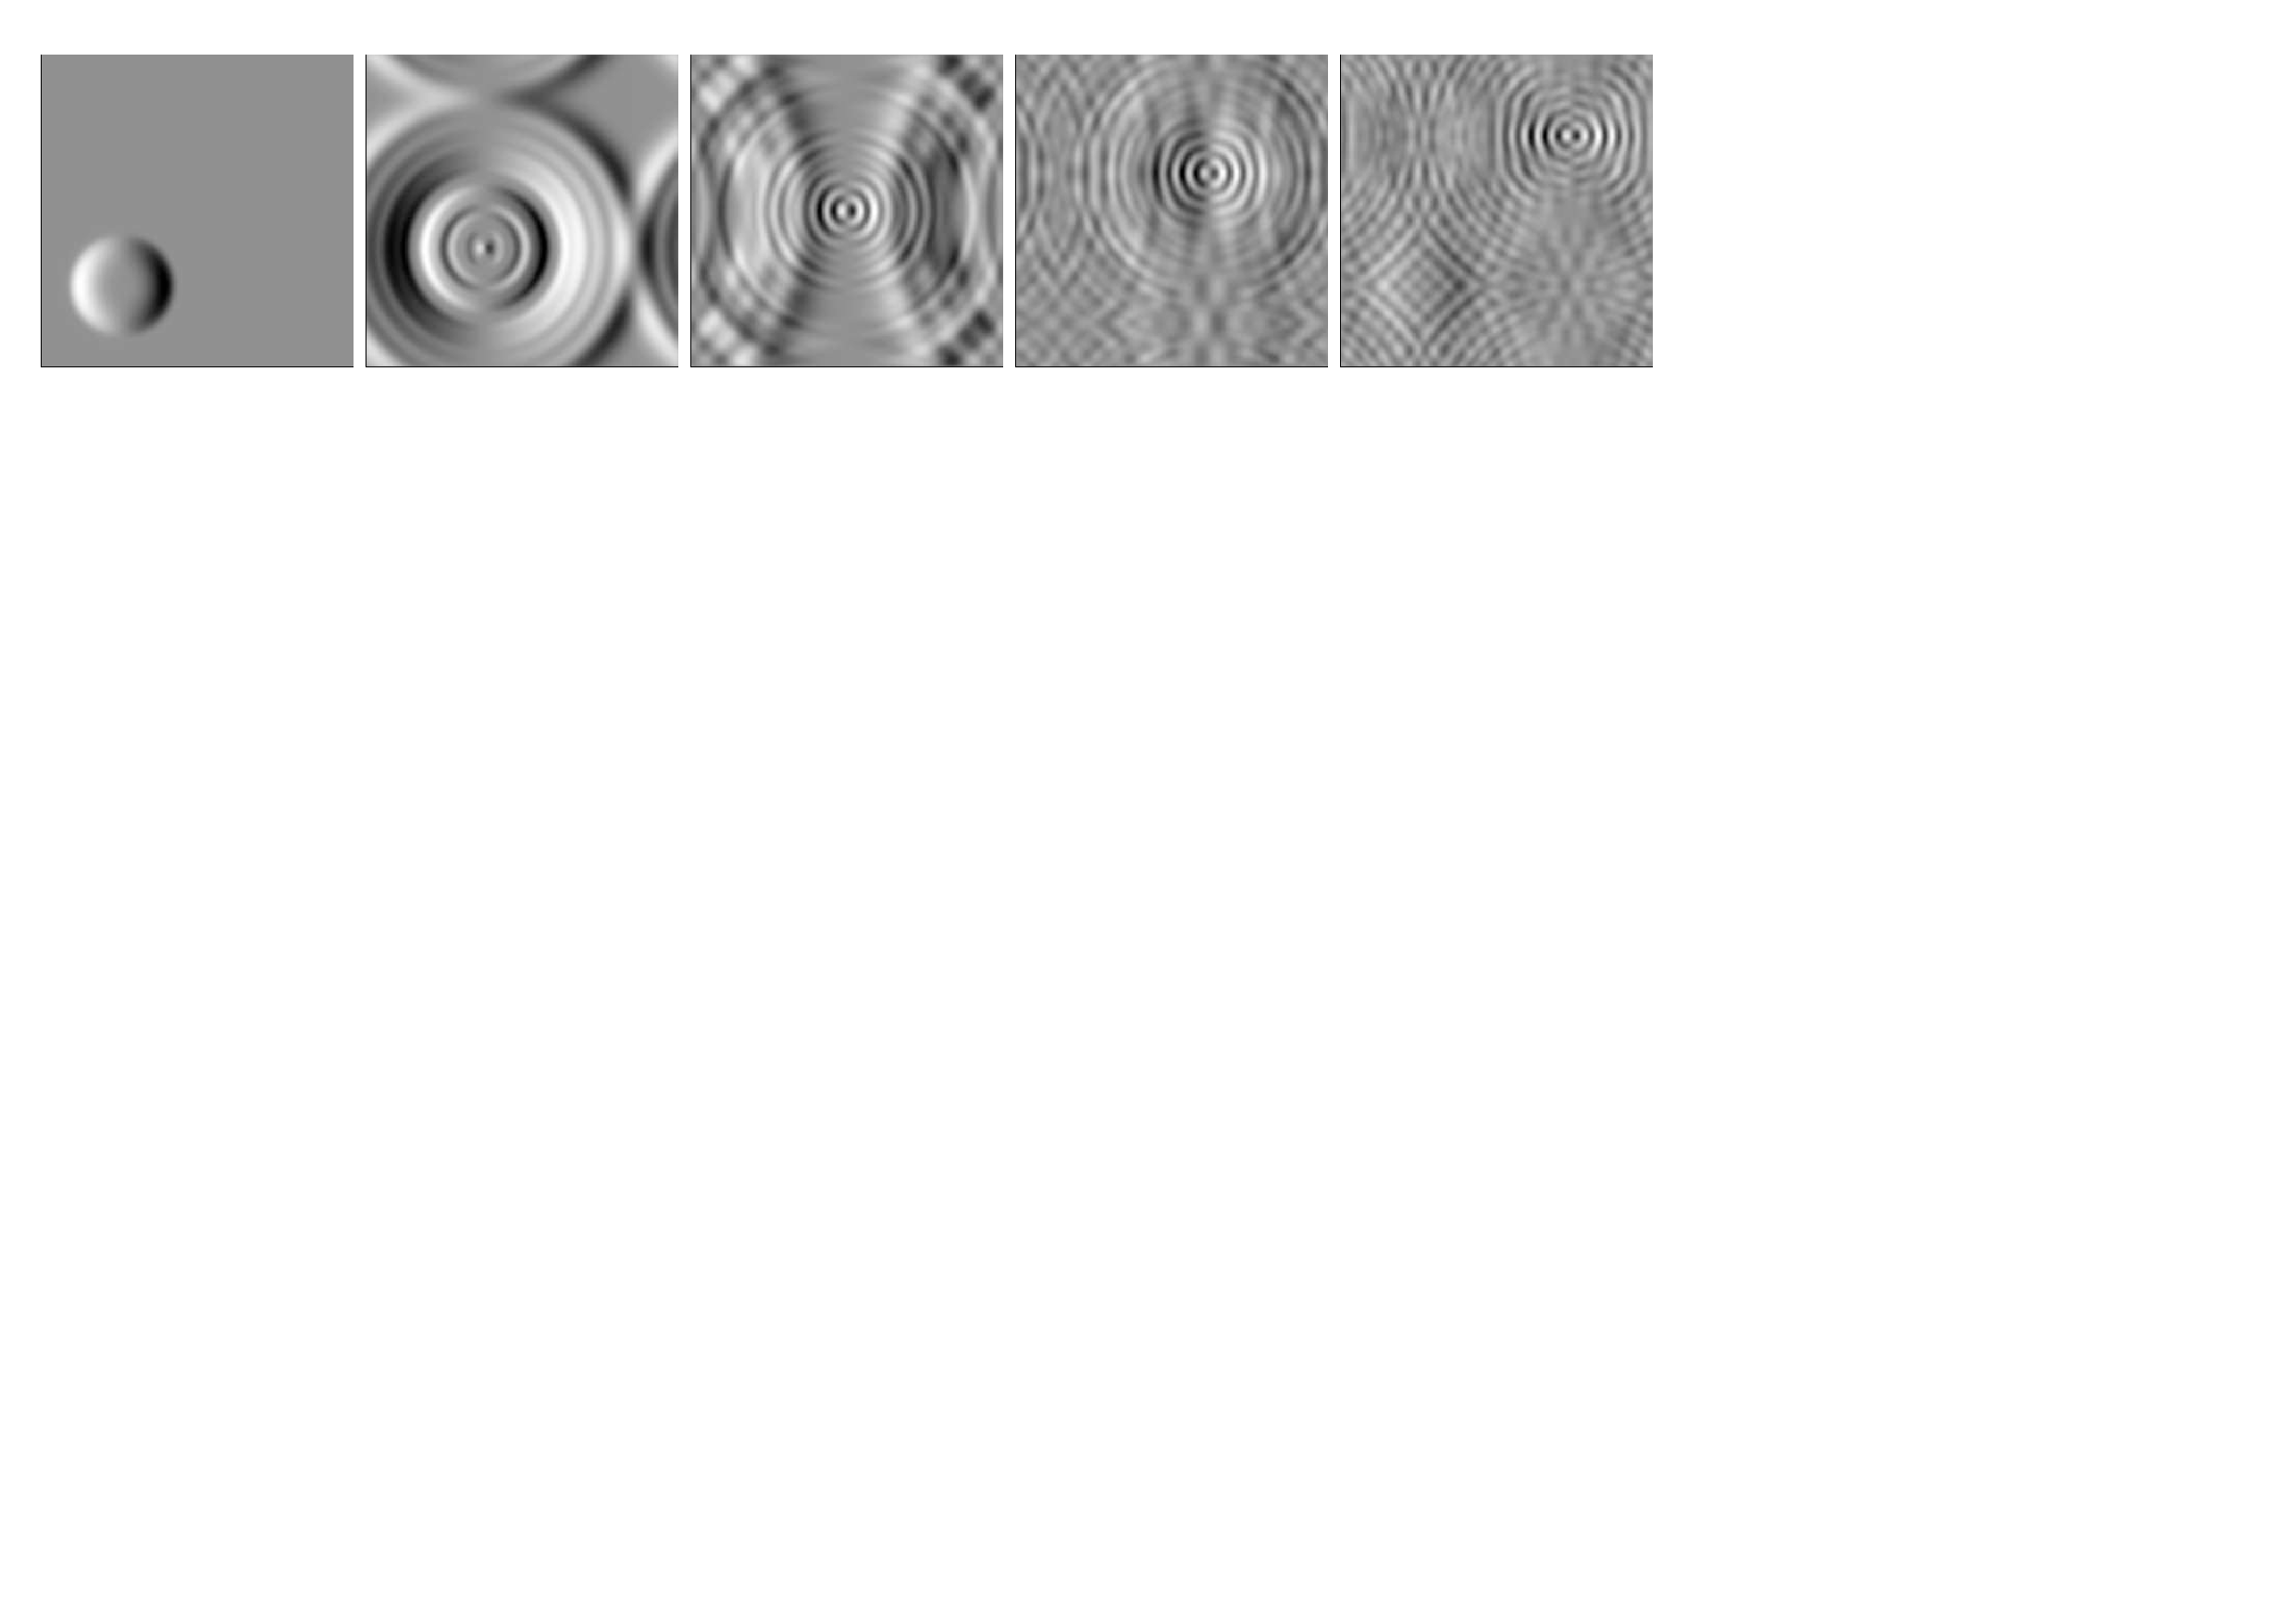
\includegraphics[angle=270,width=\textwidth]{hyperbolic.pdf}
\end{center}
\end{figure}
\maketitle
\tableofcontents
\newpage

\section{Introduction}
 Whilst many wonderful commercial software packages exist for visualising scientific
data (such as the widely used Interactive Data Language), I found that such packages
could be somewhat cumbersome for the manipulation and visualisation of my SPH data. The
main problem was that much of what I wanted to do was fairly specific to SPH (such as
interpolation to an array of pixels using the kernel) and whilst generic routines exist
for such tasks, I could not explain how they worked, nor were they
particularly fast and whilst interactive gizmos are handy, it can prove more difficult to perform the
same tasks non-interactively, as required for the production of animations. 
In fact I have found that the major
work in the visualisation of SPH data is not the image production itself but the
manipulation of data prior to plotting. Much of this manipulation makes sense
within an SPH framework (for example the interpolation provided by the kernel
and rotation of the particles for perspective).

 SPLASH is designed for this specific task - to use SPH tools to analyse SPH data and to make this a
straightforward task such that publishable images and animations can be obtained
as efficiently as possible from the raw data with a minimum amount of effort
from the user. I have found in the process that the development of powerful
visualisation tools has enabled me to pick up on effects present in my
simulation results that I would not otherwise have noticed (in particular the
difference between a raw particle plot and a rendered image can be substantial). Part of the goal of
SPLASH is to eliminate the use of crap-looking particle plots as a means of representing SPH data!

\subsection{What it does}
SPLASH is a utility for visualisation of output from (astrophysical) simulations using the
Smoothed Particle Hydrodynamics (SPH) method in one, two and three dimensions.
It is written in Fortran 90/95 and
utilises PGPLOT subroutines to do the actual plotting. In particular the following
features are included:
\begin{itemize}
\item Rendering of particle data to an array of pixels using the SPH kernel
\item Cross-sections through 2D and 3D data (as both particle plots and rendered
images).
\item Fast projections through 3D data (ie. column density plots, or integration of
other quantities along the line of sight)
\item Surface renderings of 3D data
\item Vector plots of the velocity (and other vector quantities), including vector
plots in a cross section slice in 3D.
\item Rotation and fly-throughs (multiple cross-section slices) of 3D data.
\item Automatic stepping through timesteps, making animations simple to produce.
\item Interactive mode for detailed examination of timestep data (e.g. zooming,
rotating, plotting particle labels, working out the gradient of a line, stepping forwards/backwards
through timesteps)
\item Multiple plots on page, including option to automatically tile plots if $y-$ and $x-$ limits
are the same.
\item Plot limits can be fixed, adaptive or particle tracking. Also simple to change
axes to log, invert, square root or absolute of a quantity.
\item Exact solutions for common SPH test problems (e.g. hydrodynamic shock tubes,
polytropes).
\item Calculation of quantities not dumped (e.g. pressure, entropy)
\item Transformation to different coordinate systems (for both coordinates and
vector components).
\item Straightforward production of GIF and Postscript images which can then be
converted into animations or inserted into \LaTeX documents.
\end{itemize}

\subsection{What it doesn't do}
At the moment SPLASH is geared towards gas dynamics
simulations with SPH and has basically grown out of my visualisation needs.
Thus it may not be particularly useful for things like water and solids etc. in SPH.

\subsection{SPLASH, the paper}
 The algorithms implemented in SPLASH are not described here, but instead described in a paper \citep{splashpaper} (Publications of the Astronomical Society of
 Australia, 24, 159-173), available from:

\url{http://arxiv.org/abs/0709.0832}

\noindent This paper should be cited whenever you use SPLASH for scientific purposes.

\subsection{Version History}

\begin{tabular}{|l|l|p{0.75\textwidth}|}
\hline
0.666 & 10/04 & This version was released to one or two people and had some bugs still
buried. \\

0.667 & 12/04 & This version has been released to a limited number of people who have
specifically requested a copy. \\

1.0 & 17/04/05 & first "official" release: version given to many people at IPAM meeting and
put on web.\\

1.0.1 & 17/05/05 & better colour bar behaviour on multiplots; various minor improvements \\
1.0.2 & 01/06/05 & much improved ascii data read; better line plotting; zoom on powerspectrum plots; calculate quantities switch + various bug fixes \\
1.0.3 & 05/07/05 & rescale data option; better page setup; improved zooming; interactive particle tracking + various minor changes and bug fixes \\
1.0.4 & 17/08/05 & better colour schemes; interactive colour scheme changing; various minor changes and bug fixes \\
1.0.5 & 28/09/05 & error calculation for exact solutions; legend for plot markers; exact(densityprofiles) added; more colour schemes; unit rescaling improved; other minor changes and bug fixes \\
1.5 & 17/03/06 & 3D perspective added, 3D opacity rendering, improved rotation, colour schemes, adjustable vector arrows (+legend), improved timestepping behaviour, speed enhancements, physical unit rescaling \\
1.5.1 & 26/04/06 & docs updated for v1.5, other minor changes \\
1.5.2 & 11/05/06 & S) option for saving limits and defaults; MUCH faster interactive replotting (no unnecessary re-rendering); a few other minor things \\
1.5.3 & 03/07/06 & minor bug fixes/improvements to multiple plots per page, colour bar labelling, tiled plots and legend. Accelerated rendering option for projections \\
1.5.4 & 06/07/06 & Handles multiple SPH/non-SPH particle types; axes redrawn after plotting; minor bug fixes \\
1.6 & 11/08/06 & interactive mode on multiple plots per page; highly optimised interpolation + parallel version; new Makefile; various bug fixes \\
1.6.1 & 24/08/06 & bug fixes to 1.6.0; further improvements to interactive mode on multiplots \\
1.6.2 & 24/10/06 & fast particle plotting and streamline plotting implemented; more bug fixes with interactive mode on multiplots; various other bug fixes \\
1.7.0 & 13/12/06 & renamed SPLASH instead of SUPERSPHPLOT; much faster data read for gadget and sphNG reads (only required columns read); physical units can be saved to file; new menu formats; various other bug fixes \\
1.7.1 & 04/01/07 & command line options for defaults and limits files added; minor bug fixes \\
1.7.2 & 19/02/07 & Menu shortcuts implemented; bug fix/ more sensible transformation of angular vector components in different co-ordinate systems; improvements to interactive zoom and origin recentreing; improved colour-by-type option; restrictions on page size removed; minor bug fixes \\
1.8.0 & 15/03/07 & hidden particles not used in rendering; units for z integration addded; a) and g) implemented in interactive mo  de for multiple-plots-per-page; improved cross section using x in interactive mode \\
1.8.1 & 28/03/07 & option to hide vector arrows where there are no particles added; smoother 3D plotting at low pixel numbers; (smoother vector plots); bug fixes with a); issues with round-off error with z integration of vectors fixed \\
1.9.0 & 21/05/07 & animation sequences implemented; origin settings now affect radius calculation and are relative to tracked particle; automatic line width choice for postscript devices; w key adapts vector arrows; vastly improved userguide \\
1.9.1 & 11/07/07 & environment variables + improvements to gadget data read; better prompting; 3 new colour schemes; improved legend/title options; other minor changes \\
1.9.2 & 12/09/07 & improvements to ascii read including asplash -e option; smarter foreground/background colour changing for titles; min=max problem fixed (caught by splash not pgplot); fixed vector arrow length option; other minor changes and bug fixes \\
1.10.0 & 29/11/07 & horizontal colour bars implemented; -p, -o command line options; can have mixed types in data reads; TIPSY and DRAGON data reads; density weighted rendering; normalisation option applies to column density plots; improved particle tracking; save as option; various bug fixes \\
1.10.1 & 11/03/08 & "splash to" command line option converts binary dumps to ascii format; vector plots + rotation now implemented; block labelled GADGET format read; ring-spreading exact solution added; other minor changes \\
1.10.2 & 08/05/08 & disc surface density / toomre q parameter plotting added; flash colour schemes added; splash to binary convert option; can change order in which particle types are plotted; splash.columns file overrides default column label settings; vanaverbeke format read; various bug fixes \\
1.11.0 & 15/08/08 & ability to use subset of particles in restricted parameter range(s); probability density function plot option; plot-hugging colour bars added; ability to annotate plot with a range of shapes; v, V, w and H implemented in interactive mode for >1 panel; various bug fixes \\
1.11.1 & 13/10/08 & [2] \

\hline
\end{tabular}

\subsection{Licence}
SPLASH - a visualisation tool for SPH data \copyright 2005-2007 Daniel Price.
 This program is free software; you can redistribute it and/or modify it under the terms of the GNU General Public License as published by the Free Software Foundation; either version 2 of the License, or (at your option) any later version. This program is distributed in the hope that it will be useful, but WITHOUT ANY WARRANTY; without even the implied warranty of MERCHANTABILITY or FITNESS FOR A PARTICULAR PURPOSE.  See the GNU General Public License for more details. You should have received a copy of the GNU General Public License along with this program; if not, write to the Free Software Foundation, Inc., 59 Temple Place, Suite 330, Boston, MA  02111-1307  USA.

\section{Getting started}
\subsection{Compiling the code}
The basic steps for installation are as follows:
\begin{enumerate}
\item make sure you have a Fortran 95 compiler (such as g95)
\item make sure you have the PGPLOT libraries installed
\item compile SPLASH and link with PGPLOT
\item write a read\_data subroutine so that SPLASH can read your data format
\end{enumerate}

\subsubsection{ Fortran 90/95 compilers}
 By now, many Fortran 90/95 compilers exist. In terms of free ones, the g95 compiler, downloadable from:
\begin{quote}
\url{http://www.g95.org}
\end{quote}
successfully compiles SPLASH and if necessary the PGPLOT libraries.

\subsubsection{ PGPLOT}
 The PGPLOT
graphics subroutine library is freely downloadable from
\begin{quote}
\url{http://www.astro.caltech.edu/~tjp/pgplot/}
\end{quote}
or by ftp from
\begin{quote}
\url{ftp://ftp.astro.caltech.edu/pub/pgplot/pgplot5.2.tar.gz}
\end{quote}
however check to see if it is already installed on your system (if so, the libraries are
usually located in /usr/local/pgplot). For details of the actual plotting subroutines
used by the SPLASH source code, you may want to refer to the PGPLOT userguide:
\begin{quote}
\url{http://www.astro.caltech.edu/~tjp/pgplot/contents.html}
\end{quote}

\subsubsection{ Compiling and linking with PGPLOT}
For detailed instructions on compiling and linking with PGPLOT, refer to the INSTALL file in the root directory of the SPLASH distribution (or \url{http://www.astro.ex.ac.uk/people/dprice/splash/download/INSTALL}).

A successful `make' will produce only the binary corresponding to the ascii data format -- `asplash' (by convention the first letter refers to the data format for which splash has been compiled). Using `make all' will build all of the supported data formats (e.g. GADGET is `gsplash', Matthew Bate's sphNG code is `ssplash', the VINE code is `vsplash', my own format is `dsplash' etc.). 

\subsubsection{ Reading your data}
 The most important part is getting SPLASH to read *your* data format.
If you are using a publically available code, it is reasonably likely that I
have already written a read data subroutine which will read your dumps.
If not it is best to look at some of the other examples and change the 
necessary parts to suit your data files. Note that reading directly from
unformatted data files is *much* faster than reading from formatted (ascii)
output.   

I have supplied subroutines for reading output from the publically available
GADGET code (\verb+read_data_gadget.f90+), for GASOLINE (\verb+read_data_tipsy.f90+), VINE (\verb+read_data_VINE.f90+), DRAGON (\verb+read_data_dragon.f90+) and also for Matthew Bate's sphNG code (\verb+read_data_sphNG.f90+) which is widely used in the UK. Another example of a
data read which I use is given in \verb+read_data_dansph.f90+.

Further details on writing your own subroutine are given in
appendix~\ref{sec:writeyourown}. The *easiest* way is to email me a sample data file and the subroutine
you used to write it and I can then create a data read for your file format (I won't mind).

\subsection{Environment variables}
\label{sec:envvariables}

\subsubsection{ PGPLOT}
 Several useful environment variables can be set for PGPLOT and several of them
are very useful for SPLASH. In a tcsh shell type:
\begin{verbatim}
setenv PGPLOT_DEV /xwin
setenv PGPLOT_BACKGROUND white
setenv PGPLOT_FOREGROUND black
\end{verbatim}
The first command sets the default device to the X-window, rather than the /null
device. The latter two commands set the background and foreground colours of the
plotting page. Note that these environment variables should be set \emph{before}
invoking splash (it is simplest to set them upon starting the shell by placing
them in your .tcshrc or bash/sh equivalent file). For other environment
variables which can be set, refer to the PGPLOT user guide.

\subsubsection{ Endian changing}
 On some compilers, the endian-ness (byte order) of the file read for unformatted (binary) data files can also be changed at runtime. This is useful for looking at files on different systems to the one on which they were created (e.g. x86 machines create little-endian files by default, whereas IBM/powerpc machines create big-endian).
 
  Using g95, the relevant environment variable is
\begin{verbatim}
setenv G95_ENDIAN 'BIG'
\end{verbatim}
or 'LITTLE' as appropriate. With the ifort compiler, the equivalent is:
\begin{verbatim}
setenv F_UFMTENDIAN 'big'
\end{verbatim}
or 'little'. 

 For compilers without this feature, almost all can change the endian-ness at compile time, and the appropriate flags for doing so can be set using
\begin{verbatim}
setenv ENDIAN 'BIG'
\end{verbatim}
or LITTLE before \emph{compiling} splash (this adds the appropriate compile-time flags for the compiler selected using the SYSTEM environment variable in the SPLASH Makefile). 

\subsubsection{ Ascii data read}
\label{sec:asplash}
 For several data reads there are environment variables which can be set at runtime which are specific to the data read. For the
 ascii data read (`asplash') these are:\newline

\begin{tabular}{p{0.35\textwidth}p{0.55\textwidth}}
ASPLASH\_NCOLUMNS & if given a value $>$0 sets the number of columns to be read from ascii data (overrides the automatic number of
columns determination)
\end{tabular}

\subsubsection{ Gadget data read}
\label{sec:gsplash}
 For the gadget read (`gsplash') the environment variable options are:\newline

\begin{tabular}{p{0.35\textwidth}p{0.55\textwidth}}
GSPLASH\_USE\_Z & if `YES' or `TRUE' uses the redshift in the legend instead of code time \\
GSPLASH\_DARKMATTER\_HSOFT & if given a value $>$ 0.0 will assign a smoothing length to dark matter particles for which rendered plots of column density can then be made.
\end{tabular}

\subsubsection{ sphNG data read}
 For the sphNG read (`ssplash') the environment variable options are:\newline

\begin{tabular}{p{0.35\textwidth}p{0.55\textwidth}}
SSPLASH\_CENTRE\_ON\_SINK & if `YES' or `TRUE' resets the positions such that the sink particle is positioned at the origin (applies only where there is one, and only one, sink particle present)\\
SSPLASH\_RESET\_CM & if `YES' or `TRUE' resets the positions such that the centre of mass is exactly at the origin.
\end{tabular}

\subsubsection{ Stephan Rosswog data read}
 For the srosph read (`rsplash') the environment variable options are:\newline

\begin{tabular}{p{0.35\textwidth}p{0.55\textwidth}}
RSPLASH\_FORMAT & can be `MHD' or `HYDRO' which read the appropriate data format from either the MHD or hydrodynamic codes \\
RSPLASH\_RESET\_COM & if `YES' or `TRUE' resets the positions such that the centre of mass is exactly at the origin. \\
RSPLASH\_COROTATING & if `YES' or `TRUE' then velocities are transformed to corotating frame \\
RSPLASH\_HFACT & can be changed to give correct parameter in $h=h_{fact}(m/\rho)^{1/3}$ used to set the particle masses when rendering minidumps (ie. when the mass is not dumped). Default is RSPLASH\_HFACT=1.5
\end{tabular}

\subsubsection{ Dragon data read}
 For the DRAGON read (`dsplash') the environment variable options are:\newline

\begin{tabular}{p{0.35\textwidth}p{0.55\textwidth}}
DSPLASH\_EXTRACOLS & specifies number of extra columns present in the file which are dumped after the itype array
\end{tabular}

\section{Basic SPLASH usage}
\label{sec:basic}

\subsection{Simple two column plot}
 Once you have successfully compiled SPLASH with a read data file that will read your data format,
SPLASH is invoked with the name of the data
file(s) on the command line, e.g.
\begin{verbatim}
splash myrun*.dat
\end{verbatim}
where splash should be replaced with `asplash', `gsplash' etc. depending on the data format. \\

After a successful data read, the menu should appear as something like the
following (the example given is for a ``minidump'' from Stephan Rosswog's SPH code):
\begin{verbatim}
dprice$ rsplash minidump.00001 
\end{verbatim}
\begin{verbatim}
    _                                                 _  
   (_)   _               _           _         _     (_)_
      _ (_)    ___ _ __ | | __ _ ___| |__     (_)   _  (_)
   _ (_)  _   / __| '_ \| |/ _` / __| '_ \       _ (_)    
  (_)  _ (_)  \__ \ |_) | | (_| \__ \ | | |  _  (_) _    
      (_)  _  |___/ .__/|_|\__,_|___/_| |_| (_)  _ (_)   
          (_)  (_)|_| (_) (_)  (_)(_) (_)(_) (_)(_)     

  ( B | y ) ( D | a | n | i | e | l ) ( P | r | i | c | e )

...etc...
\end{verbatim}
\begin{verbatim}
 You may choose from a delectable sample of plots 
-------------------------------------------------------
  1) x                     7) particle mass       
  2) y                     8) B\dx                
  3) z                     9) B\dy                
  4) h                    10) B\dz                
  5) \gr                  11) div B               
  6) T                   
-------------------------------------------------------
 12) multiplot [  4 ]      m) set multiplot 
-------------------------------------------------------
 d(ata) p(age) o(pts) l(imits) le(g)end h(elp)
 r(ender) v(ector) x(sec/rotate) s,S(ave) q(uit)
-------------------------------------------------------
Please enter your selection now (y axis or option):
\end{verbatim}
The simplest plot is of two quantities which are not both coordinates. For
example, to plot density vs smoothing length, type
\begin{verbatim}
Please enter your selection now (y axis or option): 5
(x axis) (default=1): 4
 Graphics device/type (? to see list, default /xwin): /xw
\end{verbatim}
 The \verb+default=+ refers to the default value assigned if you just press the return key. The last prompt asks for the PGPLOT device to which output should be directed. A full list of available graphics devices is given in the PGPLOT user guide. Some of the most useful devices are given in table \ref{tab:devices}. In the
above we have selected the X-window driver which means that the output is sent to the
screen (provided X-windows is running), as demonstrated in the screenshot shown in Figure \ref{fig:rhoh}. 

 Many useful tasks can now be achieved by moving the mouse to the plot window and selecting areas or pressing keystrokes -- this is ``interactive mode''. Pressing `h' in the plot window shows (in the terminal) the full list of commands. Of the more useful ones are: pressing `l' with the mouse over the colour bar to use a logarithmic axis, press 'a' on either the colour bar or inside the plot to adapt the plot limits, select an area with the mouse to zoom. See also \S\ref{sec:interactive}.

To exit the plot, move the mouse to the plot window and press 'q' (quit). To exit splash altogether press 'q' again from the splash main menu (in the terminal). 
\begin{figure}[ht]
\begin{center}
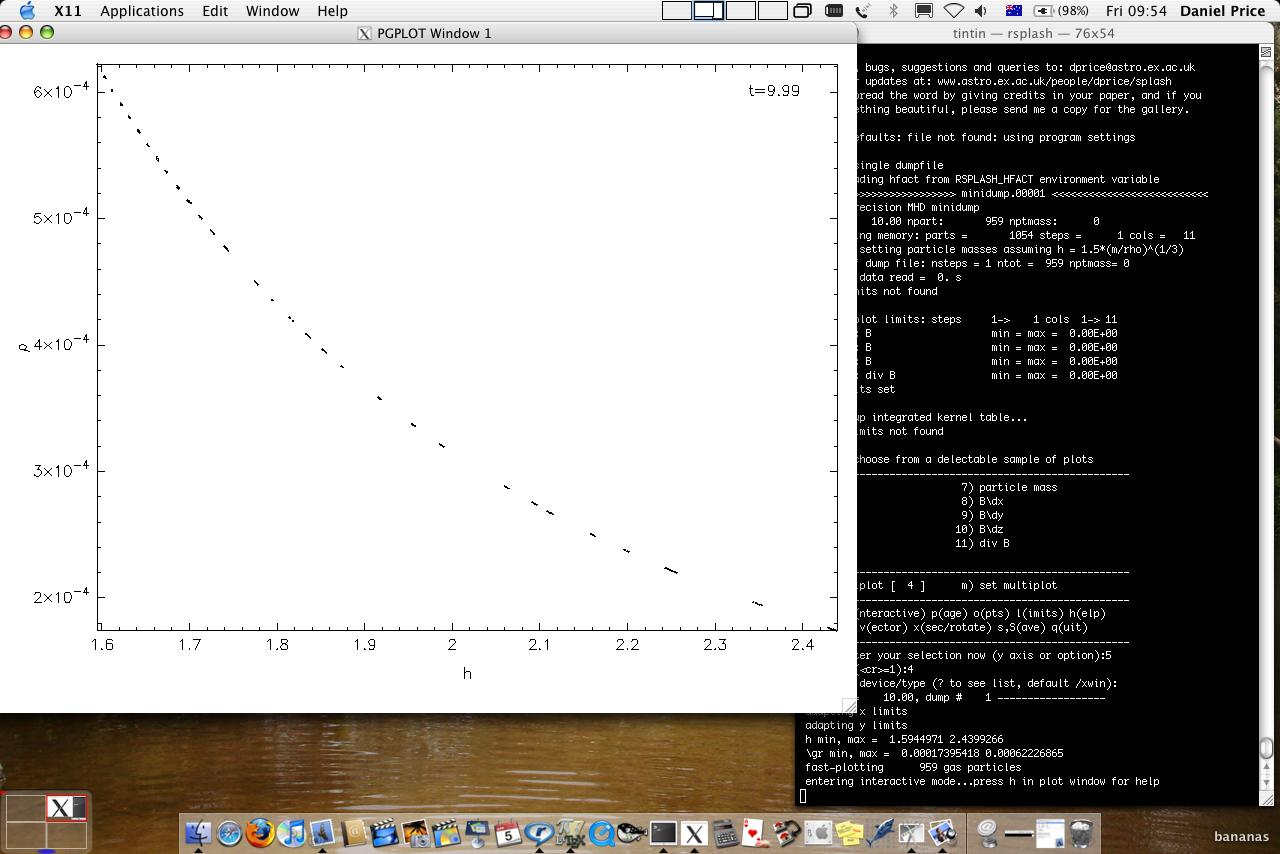
\includegraphics[width=0.8\textwidth]{rhoh.jpg}
\caption{Screenshot of simple two column plot to an X-window}
\label{fig:rhoh}
\end{center}
\end{figure}

\begin{table}[h]
\centering
\begin{tabular}{|l|l|l|l|}
\hline
\verb+/xw+, \verb+/xwin+ & X-Window (interactive) & \verb+/gif+ & GIF \\
\verb+/ps+ & Postscript (landscape) & \verb+/png+ & PNG (if installed) \\
\verb+/vps+ & Postscript (portrait) & \verb+/null+ & null device (no output) \\
\verb+/cps+ & Colour Postscript & & \\
\hline
\end{tabular}
\caption{Commonly used graphics devices available in PGPLOT}
\label{tab:devices}
\end{table}

\subsection{Rendered plots}
\label{sec:renderplot}
A more complicated plot is where both the $x-$ and $y-$ axes refer to coordinates. For example
\begin{verbatim}
Please enter your selection now (y axis or option):2
(x axis) (default=1): 1
(render) (0=none) ([0:11], default=0):5
(vector plot) (0=none, 8=B) ([0:8], default=0):0
Graphics device/type (? to see list, default /xwin): /xw
\end{verbatim}
Notice that in this case that options appeared for rendered and vector plots. Our choice of ``5'' at the (render) prompt corresponds to column 5, which in this case is the density, producing the plot shown in the screenshot in Figure~\ref{fig:renderplot}.
\begin{figure}[h]
\begin{center}
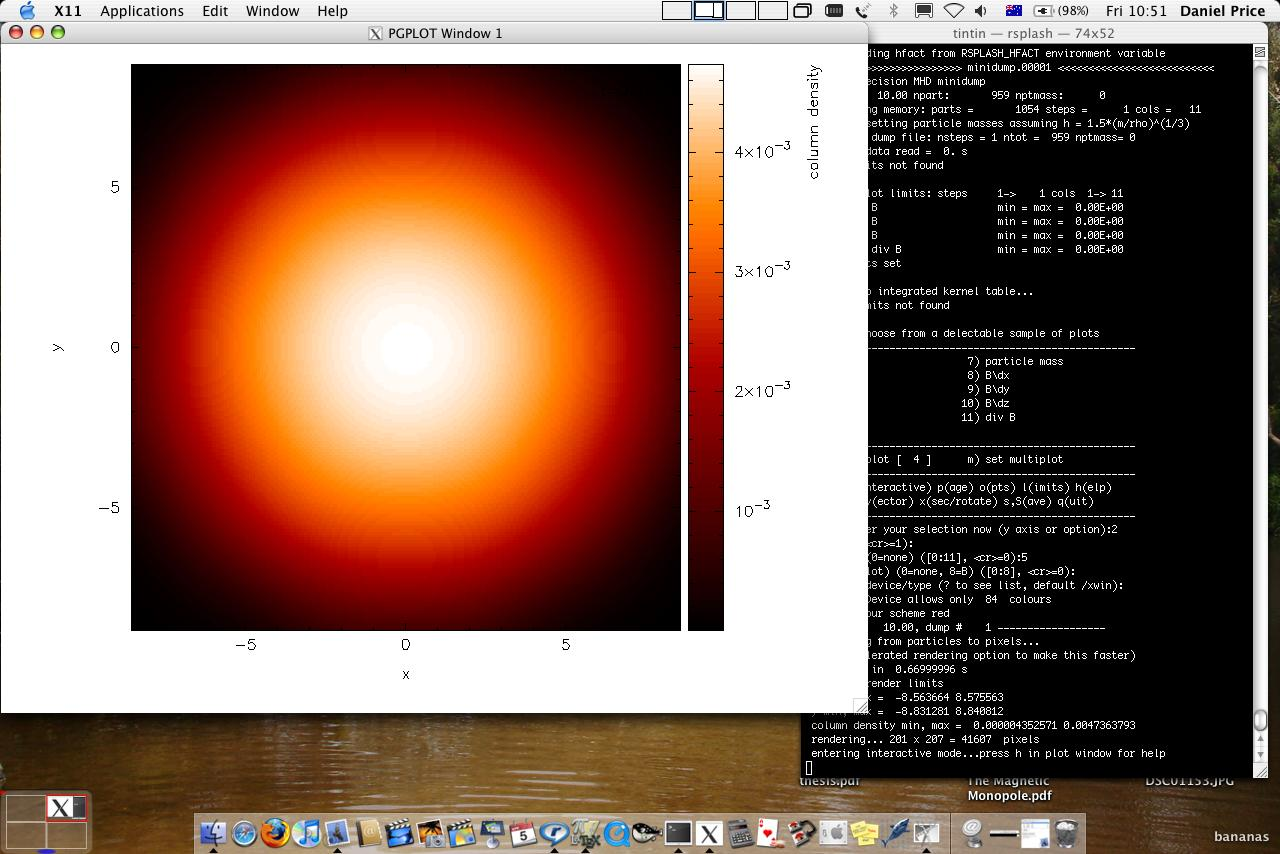
\includegraphics[width=0.8\textwidth]{renderplot.jpg}
\caption{Screenshot of 3D column density plot to an X-window}
\label{fig:renderplot}
\end{center}
\end{figure}

 Note that the render prompts only appear if, in the read\_data subroutine, values are set for the integer parameters irho, ipmass and ih corresponding to the locations of density, particle mass and smoothing length in the data arrays and provided the number of coordinate dimensions is 2 or greater (SPLASH can be used for SPH codes in 1, 2 and 3 dimensions and even for plotting ascii data where there are no ``coordinates'').

\subsection{Cross section slice}
To plot a cross section slice instead of a projection in 3D, type 'x' at the main menu to open the 'cross section/3D plotting options' menu and choose option 1 ``switch between cross section and projection''. Then re-plot the rendered plot again (exactly as in the previous example \S\ref{sec:renderplot}), setting the slice position at the prompt:
\begin{verbatim}
enter z position for cross-section slice: ([-8.328:8.327], default=0.000):
\end{verbatim}
which produces the plot shown in the screenshot in Figure~\ref{fig:renderplot_xsec}.
\begin{figure}[h]
\begin{center}
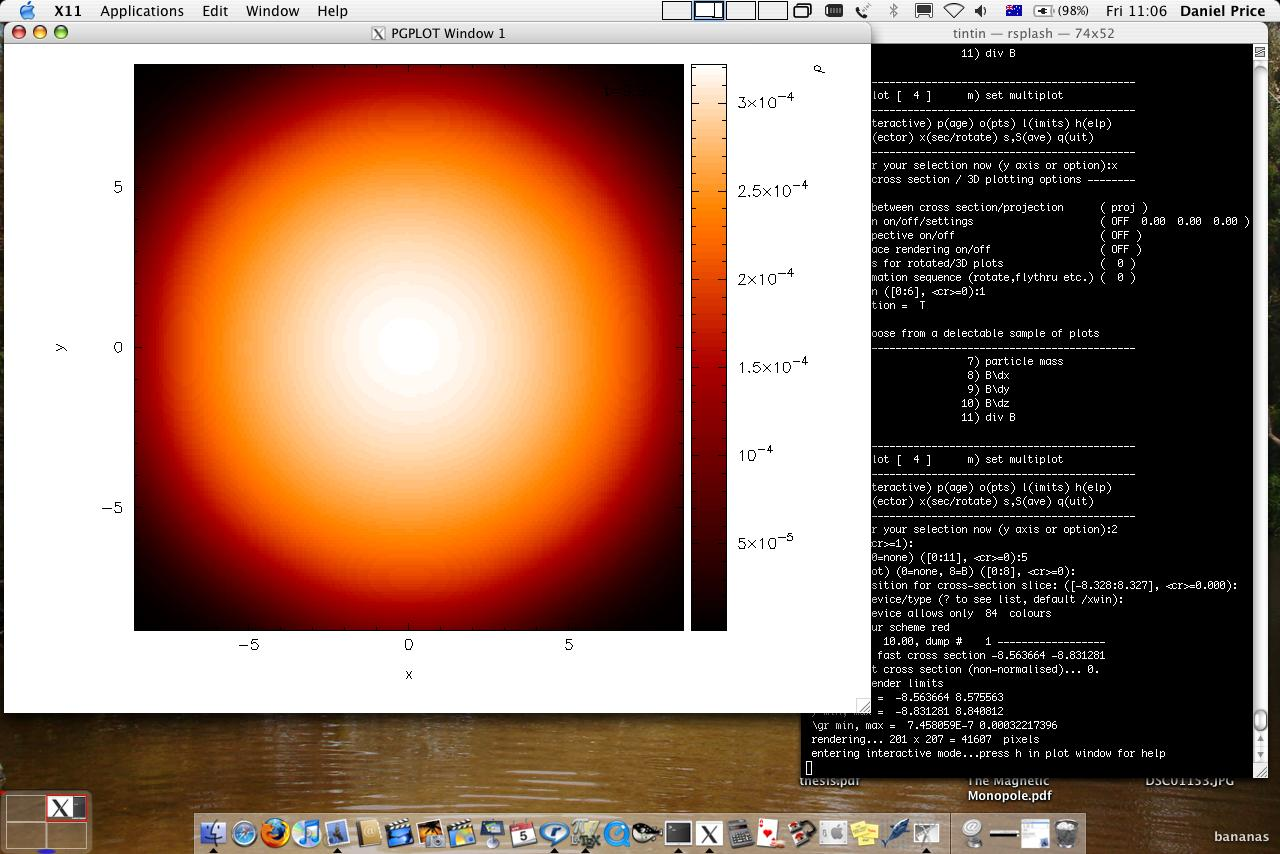
\includegraphics[width=0.8\textwidth]{renderplot_xsec.jpg}
\caption{Screenshot of 3D cross section slice plot to an X-window}
\label{fig:renderplot_xsec}
\end{center}
\end{figure}

\subsection{Vector plots}
 A prompt to plot vector arrows on top of rendered plots (or on top of particle plots) appears whenever vectors are present in the data (for details of how to specify this in your data read, see \S\ref{sec:dataread}), taking the form:
\begin{verbatim}
(vector plot) (0=none, 8=B) ([0:8], default=0):0
\end{verbatim}
where the number refers to the column of the first component of the vector quantity. 

Vector plots in 3D show either the integral of each component along the line of sight or, for cross sections, the vector arrows in a cross section slice (depending on whether a projection or cross section has been selected for 3D plots -- see the rendering examples given previously). In 2D vector plots simply show the vector arrows mapped to a pixel array using the SPH kernel.

 Settings related to vector plots can be changed via the v)ector plot submenu (\S\ref{sec:vectorplots}). The size of the arrows is set by the maximum plot limit over all of the vector components. Alternatively the arrow size can be changed interactively using 'v', 'V' (to decrease and increase the arrow size respectively) and 'w' (to automatically adjust the arrow size so that the longest arrow is of order one pixel width). 

\subsection{Moving forwards and backwards through data files}
 If you have put more than one file on the command line (or alternatively the file contains more than one dump), it is then possible to move forwards and backwards through the data by pressing the space bar with the cursor in the plot window (this is ``interactive mode''). To see the keystrokes for moving backwards or moving forwards/backwards by a specified number of steps, press 'h' in interactive mode. If you plot to a non-interactive device, SPLASH simply cycles through all the files on the command line automatically.

\subsection{Zooming in and out / changing plot limits}
 Having plotted to an interactive device (e.g. /xw), tasks such as zooming in and out, selecting, colouring and hiding particles, changing the limits of both the plot and the colour bar and many other things can be achieved using either the mouse (ie. selecting an area on which to zoom in) or by a combination of the mouse and a keystroke (e.g. move the mouse over a particle and press 'c' to see the size of the smoothing circle for that particle). One of the most useful commands in interactive mode is 'a' (adapt plot limits) which can be used to restore the plot limits to the maximum values for the data currently plotted (similarly pressing 'a' on the colour bar resets the colour bar limits to the minimum and maximum values of the rendered quantity). Pressing 'h' in interactive mode (that is, with your mouse in the plotting window) gives the full list of interactive commands (note that the text appears in the terminal from which SPLASH was invoked). Press 's' in the plot window to save changes between timesteps, otherwise the settings will revert when you move to the next timestep. 
 
 These tasks can also be achieved non-interactively by a series of drop-down submenus invoked from the main menu by typing a single character. For example limits changing options are contained in the l)imits submenu, so to manually set plot limits we would type ``l'' from the main menu, then ``2'' for option 2 (set manual limits) and follow the prompts to set the limits for a particular data column. 

\subsection{Producing a postscript figure for a paper}
 Producing a postscript plot suitable for inclusion in a \LaTeX  file is simple: at the PGPLOT device prompt, 
\begin{verbatim}
 Graphics device/type (? to see list, default /xwin):
\end{verbatim}
instead of ``/xw'' (for an X-window), simply type ``/ps'' to use the postscript driver. This produces a file which by default is called pgplot.ps. To specify both the device and filename, type ``myfile.ps/ps'' as the device. Files produced in this way can be directly incorporated into \LaTeX  using standard packages such as graphicx, psfig or epsfig (note that there are only very minor differences between a .eps file and a .ps file -- an eps file can be generated from a .ps file using ``ps2epsf'' if you really care). Options you may wish to change for postscript plots are the line width (generally 2-3 is better for visible axes in papers) and/or the character height (which sets the size of the axes labels). Both can be changed via the p)age options submenu (ie. type ``p'' from the main menu). The reason the line width is only 1 by default is that thicker line widths can look poor on output to pixel devices such as gif and png.

\subsection{Producing a sequence of plots for a movie}
\label{sec:movies} 
 In order to produce a movie of a simulation, the first step is to generate a sequence of plots corresponding to different times in the simulation. To achieve this in SPLASH, simply invoke SPLASH with all of the filenames on the command line (e.g. \verb+splash dump*+), adjust until it looks right (either interactively or using the menu options), if in interactive mode type 's' to save the current settings, then plot the same thing again but to a non-interactive device. For a movie it is best to use a pixel device such as gif or png. To do this, at the PGPLOT device prompt:
\begin{verbatim}
 Graphics device/type (? to see list, default /xwin):
\end{verbatim}
type /gif or /png (depending on which drivers have been installed in your PGPLOT installation -- typing ``?'' at this prompt shows you the list). This will generate a series of plots with names such as \verb+pgplot.gif+, \verb+pgplot.gif_2+, \verb+pgplot.gif_3+ corresponding to each new plotting page generated. To change these into more sensible names use the script provided in the splash/scripts directory (see \S\ref{sec:fixpgplotnames}). 
 
 Having obtained a sequence of images there are a variety of ways to make these into an animation using both free and commercial software. Suggestions on software packages to use for Mac, Linux and Windows can be found in the online faq (\url{http://www.astro.ex.ac.uk/people/dprice/splash/faqs.html}). I generally use the application ``graphic converter'' on Mac OS/X which makes quicktime movies from a sequence of images.
 
 
\subsection{Ten quick hints for producing good-looking plots}
In this section I have listed ten quick suggestions for simple changes to settings which can improve the look of a visualisation substantially compared to the default options. These are as follows:
\begin{enumerate}
\item {\bf Log the colour bar.} This is often the reason why your first rendered plot may look somewhat blank, especially if the simulation is dominated by a few high density objects. To do this simply move the cursor over the colour bar and hit ``l'' (for log). Alternatively log transformations can be applied to columns non-interactively via the ``apply log or inverse transformations to columns'' option in the l)imits menu.
\item {\bf Adjust the colour bar limits}. Position the mouse over the colour bar and click to set the minimum and maximum limit on the colour bar. To revert to the widest max/min possible for the data plotted, press `a' with the cursor positioned over the colour bar. Note that limits can also be set manually in the l)imits submenu.
\item {\bf Try changing the colour scheme}. Press `m' or `M' in interactive mode to cycle forwards or backwards through the available colour schemes.
\item {\bf Increase the number of pixels}. The default number of pixels along the $x-$axis is 200, chosen to allow faster interactive plotting. However, for production plots it is much better to use at least 400-500 pixels for figures to go in research papers and up to 1000-2000 for making movies (beware that using more pixels also increases the file size substantially!). Change the number of pixels using the ``change number of pixels'' option in the r)ender submenu.
\item {\bf Try using normalised interpolations}. If your simulation does not involve free surfaces (or alternatively if the free surfaces are not visible in the figure), turning the ``normalise interpolations'' option on (in the r)ender submenu) may improve the smoothness of the rendering (sometimes substantially). This is turned off by default because it leads to funny-looking edges. Note that option has no effect on 3D projection plots (where it is not meaningful to normalise the interpolation).
\item {\bf Try turning the axes off}. For movies, often axes are unnecessary and detract from the visual appeal. Axes can be turned off in the ``axes options'' option in the p)age submenu.
\item {\bf Change axes/page colours}. The background colour (colour of the page) and foreground colour (used for axes etc) can be changed vie the ``set foreground/background colours'' option in the p)age submenu. Alternatively these can be changed prior to invoking SPLASH by setting the PGPLOT\_FOREGROUND and PGPLOT\_BACKGROUND environment variables (see \S\ref{sec:envvariables}).
\item {\bf Move the legend or turn it off}. The time legend can be moved by positioning the mouse and pressing `G' in interactive mode. The legend can be turned off using the le(g)end submenu. Similarly the vector plot legend can be turned on/off in the v)ector submenu and moved by positioning the cursor and pressing `H'.
\item {\bf Use physical units on the axes}. These can be set via the d)ata submenu. See \S\ref{sec:changingunits} for more details.
\item {\bf Save settings to disk!} Don't waste your effort without being able to reproduce the plot you have been working on. Pressing `s' in interactive mode only saves the current settings for subsequent timesteps. Pressing `s' from the main menu saves these settings to disk. Pressing `S' from the main menu saves both the plot options \emph{and} the plot limits, so that the current plot can be reproduced exactly when splash is next invoked.
\end{enumerate}

\section{Changing plot settings}
 The plot settings may be changed in a series of submenus. The options set using
the submenus can be saved using the (s)ave option from the menu. This saves all of
the current options to a file called \verb+splash.defaults+ in the current directory, which is
automatically read upon starting splash the next time. To revert to default options, simply delete this file.
Pressing `S' from the main menu saves both the \verb+splash.defaults+ file and also saves the plot limits to a file called \verb+splash.limits+. This file is a simple two-column ascii file corresponding to the minimum and maximum plot limits for each column of data. Thus saving using 'S' means that exactly the same plot can be plotted next time splash is invoked, where saving using 's' means that the plot settings will be the same although the limits will be different. To reset the plot limits either adjust the limits and press 'S' again or simply delete the splash.limits file.

\subsection{set (m)ultiplot}
\label{sec:multiplot}
\subsubsection{ Plotting more than one column from the same file on the same page (multiplot)}
 Press 'm'  (``set multiplot'') from the main menu to set up a multiplot. Note that a ``multiplot'' (multiple columns plotted from the same file) is different to plotting ``multiple plots per page'' (divide the plotting page up into panels). The number of panels across and down on a page can be changed (see \ref{sec:nacrossndown}) irrespective of whether or not you are also plotting multiple columns from the same file.

Once you have gone through the options to set up a multiplot, to actually plot what you have set simply type the number of the column corresponding to ``multiplot'' at the $y-$axis prompt.

\subsection{(d)ata options}
The following can all be achieved from the d)ata options menu:

\subsubsection{ Re-reading the initial data / changing the dump file}
\label{sec:d1}
 The data can be re-read from the dump file or a new dump file can be selected by choosing  the d)ata menu, option 1 (or just ``d1'' from the main menu). In practise it is usually faster to exit splash and restart with the new dump file name on the command line (remember to save by pressing 'S' from the main menu before exiting to save both the current settings and the plot limits -- then you can continue plotting with the current settings using a new dump file).
 
 If you have placed more than one file on the command line, then pressing space in interactive mode will read (and plot) the next file (press 'h' in interactive mode for a full list of commands - you can move forwards and backwards using arbitrary jumps). For non-interactive devices or where interactive mode is turned off dump files are cycled through automatically, plotting the same plot for each file/timestep.
 
\subsubsection{ Using only a subset of data files / plotting every $n-$th dump file}
\label{sec:subsetofsteps}
 When splash is invoked with more than one filename on the command line (for example, where all files are selected with something like ``splash DUMP*'') it is often helpful to use only a subset of the files. This can be set in the d)ata menu, selecting option 2 ``change number of timesteps used''. This prompts something like:
\begin{verbatim}
 Start at timestep ([1:10], default=1):
 End at timestep ([1:10], default=10):
 Frequency of steps to read ([1:10], default=1):
\end{verbatim}
so that the beginning, end and frequency (e.g. 2 would mean read every second step) of dump files to use can be set.

 To plot a subset of the data files in *any* order, see \S\ref{sec:selectedstepsonly}. 

 Of course, another way to achieve the same thing is to explicitly order the files on the command line. A method I often use is to write all filenames to a file, e.g. 
\begin{verbatim}
ls DUMP* > filelist
\end{verbatim}
then edit the file to list only the files I want to use, then invoke splash using
\begin{verbatim}
splash `cat filelist`
\end{verbatim}
(note the direction of the quotes which is unix-speak for ``use the result of this command''). 

\subsubsection{ Plotting a subset of data files in non-sequential order}
\label{sec:selectedstepsonly}
 A subset of data files from the command line can be chosen in any order using the ``plot selected steps only'' option from the d)ata submenu, which then prompts the user to enter something like the following:
\begin{verbatim}
 Enter number of steps to plot ([1:10], default=0):5
 Enter step  1 ([1:10], default=1):5
 Enter step  2 ([1:10], default=2):2
 Enter step  3 ([1:10], default=3):1
 Enter step  4 ([1:10], default=4):4
 Enter step  5 ([1:10], default=5):3
\end{verbatim}
Note that only a limited number of steps can be selected in this way. An alternative way is to order the files on the command line before invoking splash (see \S\ref{sec:subsetofsteps}). 

\subsubsection{ Plotting more than one file without re-reading the data from disk}
\label{sec:buffering}
 For small data sets (or a small number of dump files) it is often useful to read all of the data into memory so that you can move rapidly forwards and backwards between dumps (e.g. in interactive mode, or where both dumps are plotted on the same page) without unnecessary re-reading of data from disk. This is achieved by turning ``buffering of data'' on in the d)ata menu (provided you have the memory of course!!). Non-buffered data means that only one file at a time is read.

\subsubsection{ Calculating additional quantities not dumped}
Turn ``calculate extra quantities'' on in the d)ata menu. This turns on the calculation of several additional quantities such as radius and the magnitude of all vector quantities. 

 Note that the origin for the calculation of radius can be changed via the ``rotation on/off/settings'' option in the x) submenu. If particle tracking limits are set (see \S\ref{sec:track}) the radius is calculated relative to the particle being tracked.

 At the moment it is not possible for the user to change the list of quantities from within splash (although it is on my to-do list). However, additional quantities are calculated in the subroutine \verb+calc_quantities+ in the file \verb+calc_quantities.f90+, in which it is quite a simple matter to add your own by following those already implemented. 

See also \S\ref{sec:geom} for how to transform vectors (and positions) into different coordinate systems. 

\subsubsection{ Plotting data in physical units}
\label{sec:physicalunits}
 Data can be plotted in physical units by turning on the ``use physical units'' option in the d)ata submenu. The settings for transforming the data into physical units may be changed via the ``change physical unit settings'' option in the d)ata menu. (see \S\ref{sec:changingunits})

 For some data reads (sphNG, srosph) the scalings required to transform the data into physical units are read from the dump file. These are used as the default values but are overridden as soon as changes are made by the user (that is, by the presence of a `splash.units' file) (see \S\ref{sec:changingunits}).
 
\subsubsection{ Rescaling data columns}
See \S\ref{sec:physicalunits}.

\subsubsection{ Plotting column density in g/cm$^{2}$ without having x,y,z in cm}
See \S\ref{sec:changingunits}. In addition to units for each column (and a unit for time -- see \S\ref{sec:timeunits}) a unit can be set for the length scale added in 3D column integrated plots. The prompt for this appears after the units of either $x$, $y$, $z$ or $h$ has been changed via the ``change physical unit settings'' option in the d)ata menu. The length unit for integration is saved in the first row of the splash.units file, after the units for time.

\subsubsection{ Changing physical unit settings}
\label{sec:changingunits}
The settings for transforming the data into physical units may be changed via the ``change physical unit settings'' option in the d)ata menu. To apply the physical units to the data select the ``use physical units'' option in the d)ata submenu.

 The transformation used is $new= old*units$ where ``old'' is the data as read from the dump file and ``new'' is the value actually plotted. The data menu option also prompts for a units label which is appended to the usual label. Brackets and spaces should be explicitly included in the label as required.
 
  Once units have been changed, the user is prompted to save the unit settings to a file called \verb+splash.units+. Another way of changing units is simply to edit this file yourself in any text editor (the format is fairly self-explanatory). To revert to the default unit settings simply delete this file. To revert to code units turn ``use physical units'' off in the d)ata menu.
 
 A further example of where this option can be useful is where the $y-$axis looks crowded because the numeric axis labels read something
like $1\times 10^{-4}$. The units option can be used to rescale the data so
that the numeric label reads $1$ (by setting $units=10^{4}$) whilst the label string is amended to read $y
[\times 10^{-4}]$ by setting the units label to $ [ \times 10^{-4}]$.

\subsubsection{ Changing the axis label to something like $x$ $[ \times 10^{4} ]$}
See \S\ref{sec:changingunits}.

\subsubsection{ Changing the time units}
\label{sec:timeunits}
Units for the time used in the legend can be changed using the ``change physical unit settings'' in the d)ata menu. Changing the units of column zero corresponds to the time (appears as the first row in the `splash.units' file). 

\subsection{(i)nteractive mode}
\label{sec:interactive}
 The menu option i) turns on/off interactive mode (alternatively use ``interactive mode on/off'' in the p)age submenu). With this option turned on (the default) and
an appropriate device selected (ie. the X-window, not /gif or /ps), after
each plot the program waits for specific commands from the user. With the cursor
positioned anywhere in the plot window (but not outside it!), many different
commands can be invoked. Some functions you may find useful are: Move through timesteps by pressing the space bar (press
 `b' to go back); zoom in by selecting an area with the mouse; rotate the
particles by using the $<$, $>$,[, ] and $\backslash$, / keys; log the axes by holding the cursor
over the appropriate axis and pressing the `l' key. Press `q' in the plot window
to quit interactive mode.

 A full list of these commands is obtained by holding
the cursor in the plot window and pressing the `h' key (h for help). Note that changes made in interactive mode will only be saved by pressing the
`s' (for save) key. Otherwise pressing the space bar (to advance to the next
timestep) erases the changes made whilst in interactive mode. A more limited
interactive mode applies when there is more than one plot per page.

 Many more commands could be added to
the interactive mode, limited only by your imagination. Please send me your suggestions!

\subsubsection{ Adapting the plot limits}
 Press `a' in interactive mode to adapt the plot limits to the current minimum and maximum of the quantity being plotted. With the mouse over the colour bar, this applies to the colour bar limits. Also works even when the page is subdivided into panels. To adapt the size of the arrows on a vector plot, press `w'. To use ``adaptive plot limits'' (where the limits change at every timestep), see \S\ref{sec:adapt}.

\subsubsection{ Making the axes logarithmic}
 Press 'l' in interactive mode with the mouse over either the x or y axis or the colour bar to use a logarithmic axis. Pressing 'l' again changes back to linear axes. To use logarithmic labels as well as logarithmic axes, see \S\ref{sec:loglabels}.

\subsubsection{ Colouring a subset of the particles and retaining this colour through other timesteps}
\label{sec:colourparts}

\begin{figure}
\centering
\begin{tabular}{cc}
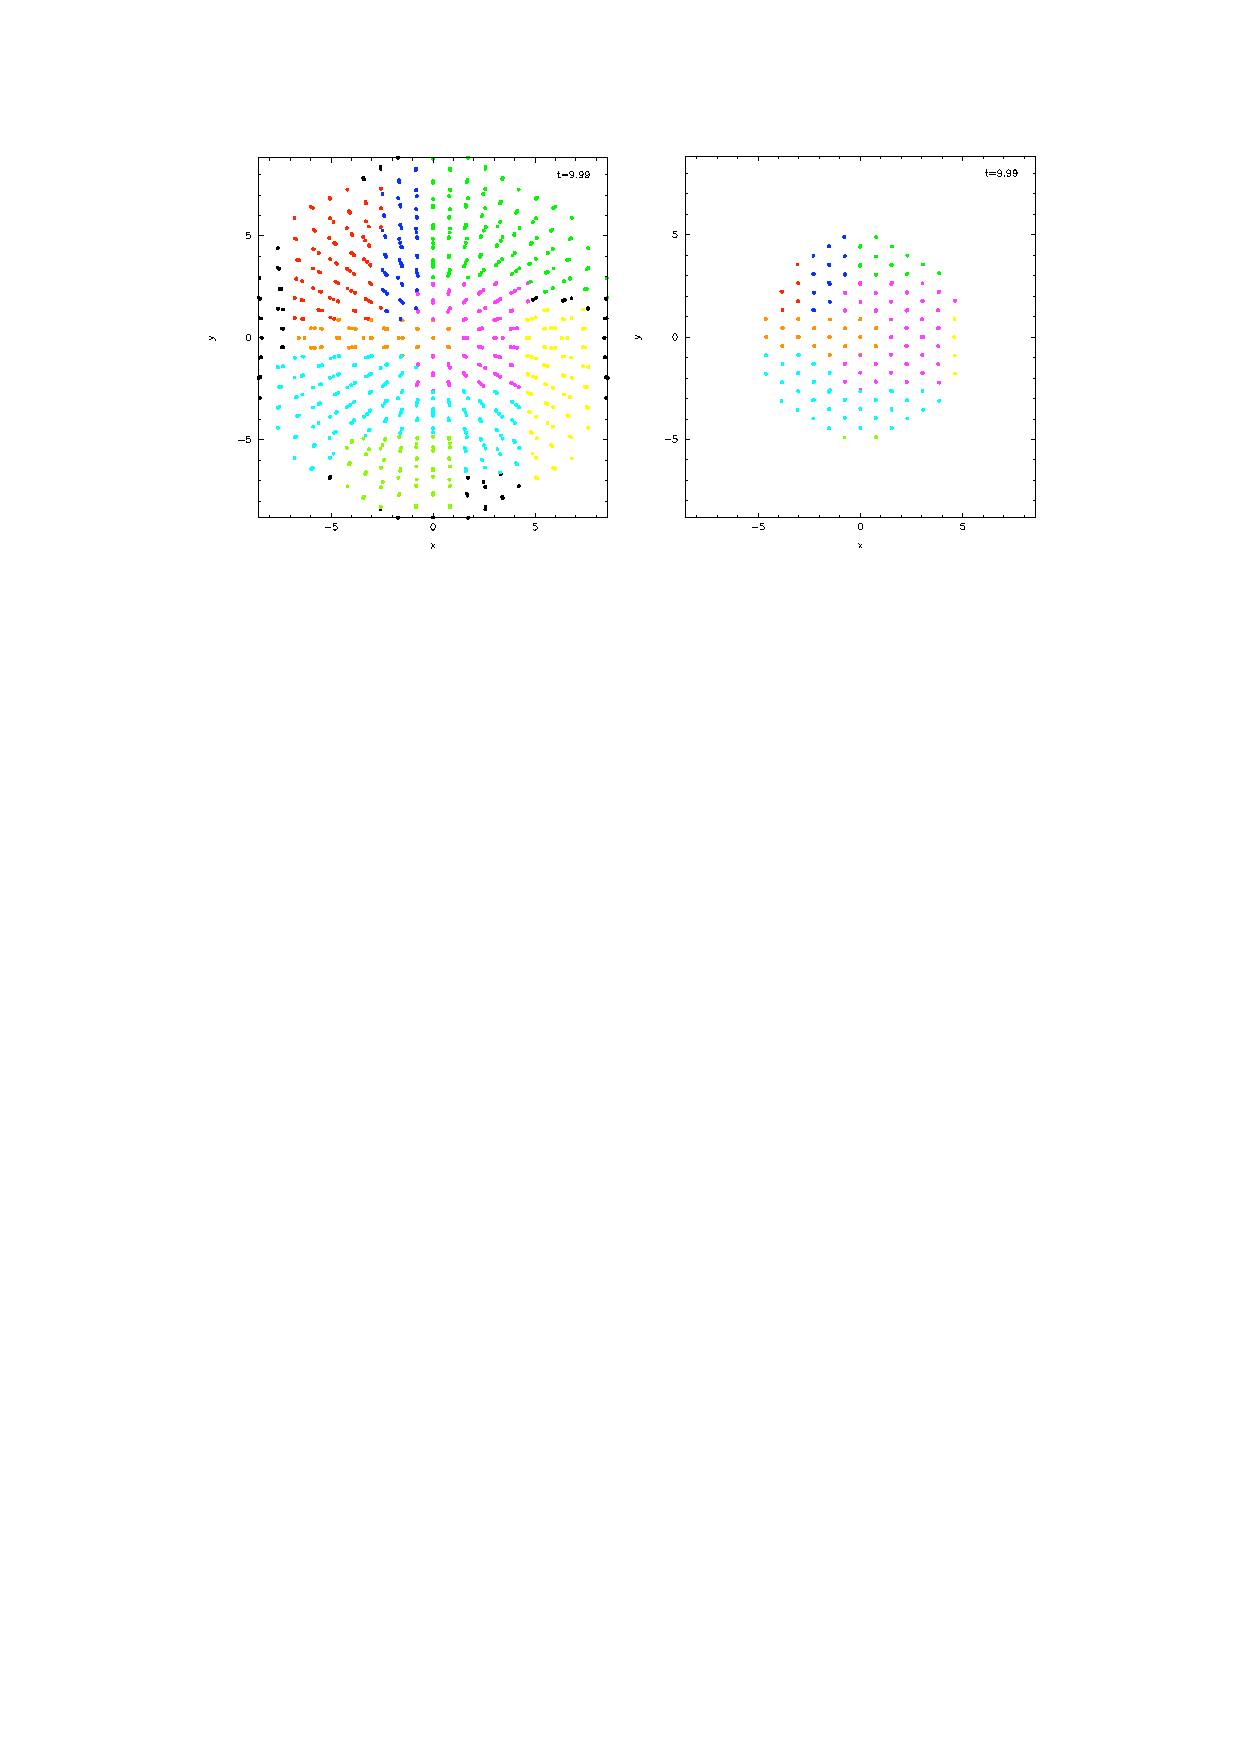
\includegraphics[angle=270,width=0.4\textwidth]{colourparts.pdf} &
\includegraphics[angle=270,width=0.4\textwidth]{colourparts_highdens.pdf}
\end{tabular}
\caption{Example of particles coloured interactively using the mouse (left) and selection using a parameter range (right), which is the same as the plot on the left but showing only particles in a particular density range (after an intermediate plot of density vs x on which I selected a subset of particles and hit 'p')}
\label{fig:colourparts}
\end{figure}

 In interactive mode, select a subset of the particles using the mouse (that is left click and resize the box until it contains the region you require), then press either 1-9 to colour the selected particles with colours corresponding to PGPLOT colour indices 1-9, press 'p' to plot only those particles selected (hiding all other particles), or 'h' to hide the selected particles. An example is shown in the left panel of Figure~\ref{fig:colourparts}.  Particles retain these colours between timesteps and even between plots. This feature can therefore be used to find particles within a certain parameter range (e.g. by plotting density with x, selecting/colouring particles in a given density range, then plotting x vs y in which the particles will appear as previously selected/coloured). An example of this feature is shown in the right panel of Figure~\ref{fig:colourparts} where I have plotted an intermediate plot of density vs x on which I selected a subset of particles and hit 'p' (to plot only that subset), then re-plotted x vs y with the new particle selections.
 
 To ``un-hide'' or ``de-colour'' particles, simply select the entire plotting area and press ``1'' to restore all particles to the foreground colour index.
 
  Particles hidden in this manner are also no longer used in the rendering calculation. Thus it is possible to render using only a subset of the particles (e.g. using only half of a box, or only high density particles). An example is shown in Figure~\ref{fig:rendersubset}.

 To colour the particles according to the value of a particular quantity, see \S\ref{sec:colournotrender}.

 Note that selection in this way is based on the particle \emph{identity}, meaning that the parameter range itself is not preserved for subsequent timesteps, but rather the subset of particles selected from the initial timestep. This can be useful for working out which particles formed a particular object in a simulation by selecting only particles in that object at the end time, and moving backwards through timesteps retaining that selection.

\subsubsection{ Working out which particles formed a particular object in a simulation}
This can be achieved by selecting and colouring particles at a particular timestep and plotting the same selection at an earlier time. See \S\ref{sec:colourparts} for details.

\subsubsection{ Plotting only a subset of the particles}
 To turn plotting of certain particle \emph{types} on and off, see \S\ref{sec:plotparticlesbytype}. To select a subset of the particles based on restrictions of a particular parameter or by spatial region see \S\ref{sec:colourparts}.

\subsubsection{ Rendering using only a subset of the particles}
\label{sec:rendersubset}
 Particles can be selected and `hidden' interactively (see \S\ref{sec:colourparts}) -- for rendered plots `hidden' particles are also not used in the interpolation calculation from the particles to the pixel array. An example is shown in Figure~\ref{fig:rendersubset}, where I have taken one of the rendered examples in \S\ref{sec:basic}, selected half of the domain with the mouse and pressed 'p' to plot only the selected particles. The result is the plot shown.
\begin{figure}[h]
\begin{center}
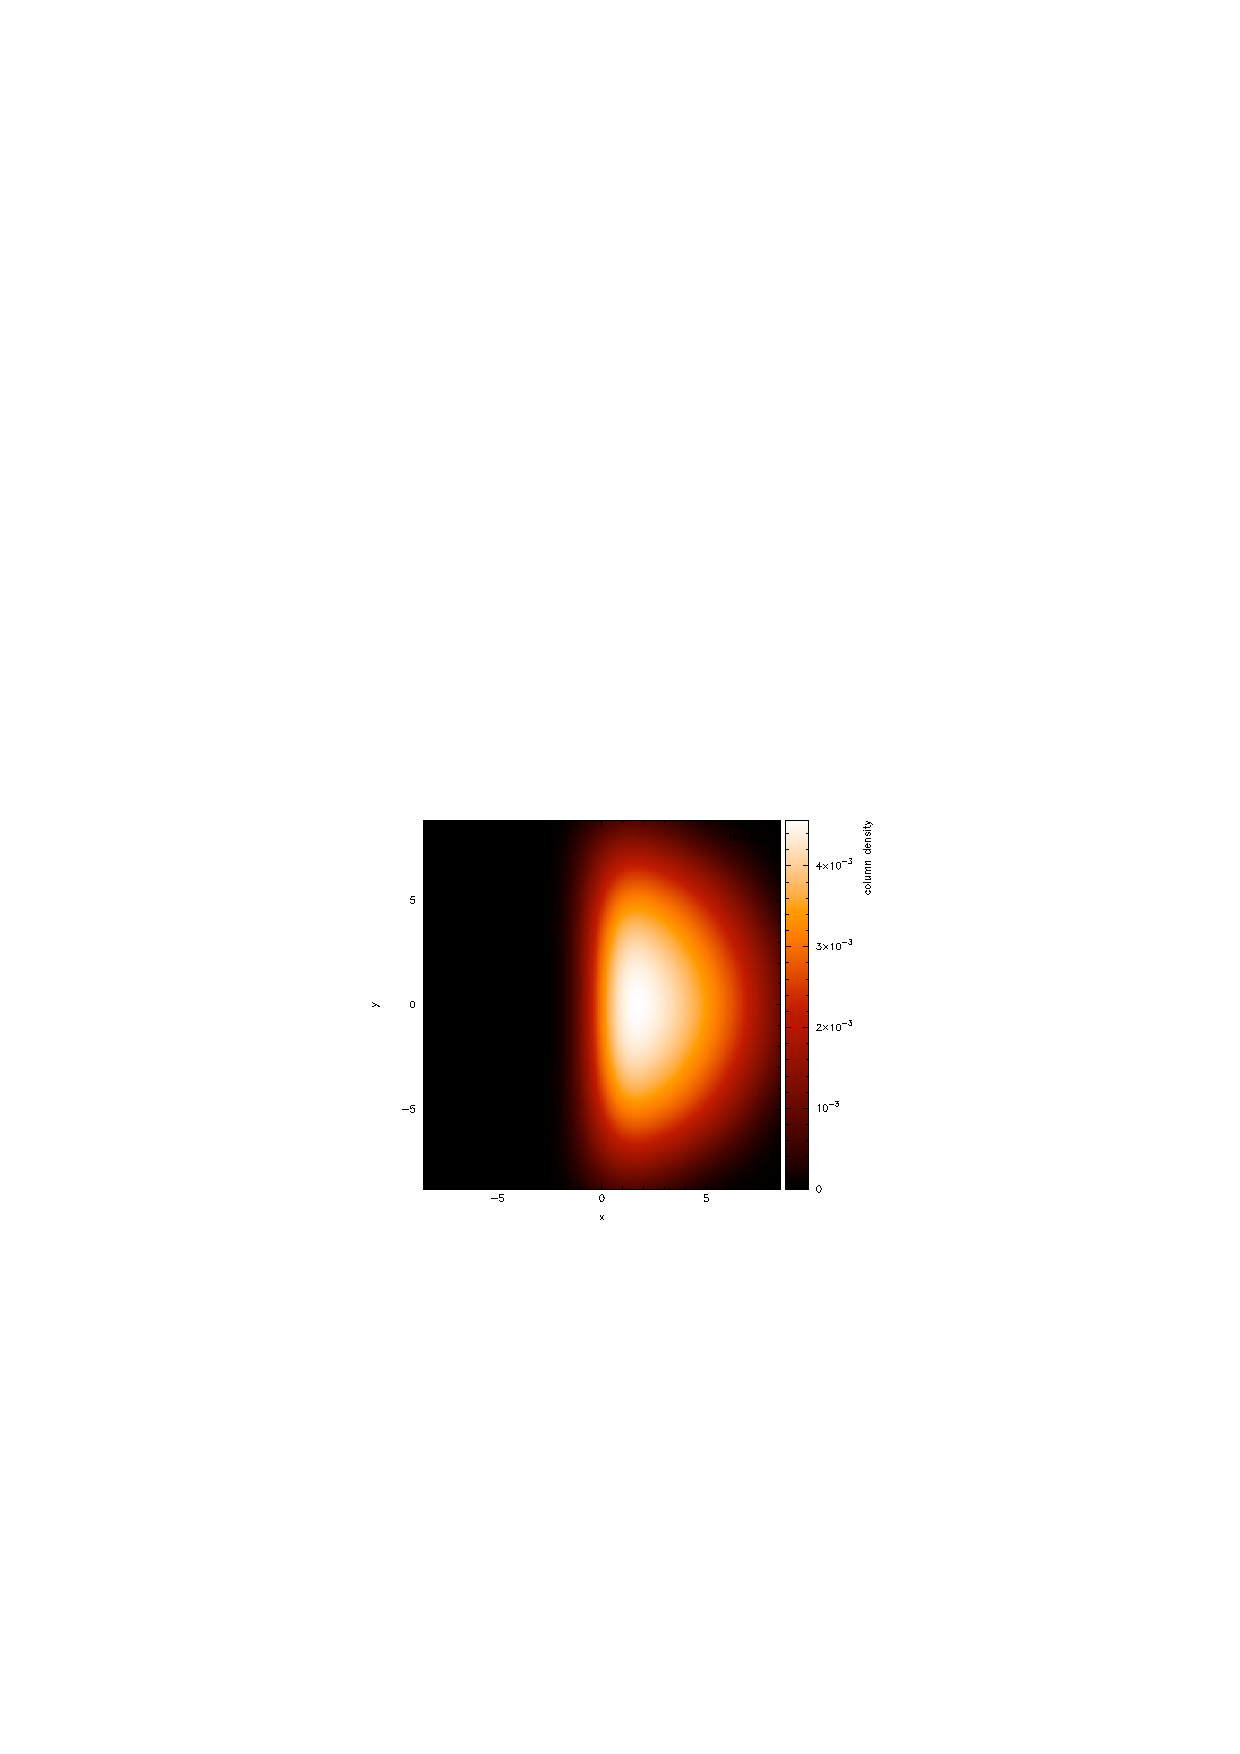
\includegraphics[angle=270,width=0.5\textwidth]{rendersubset.pdf}
\caption{Example of rendering using only a subset of the particles. Here I have selected only particles on the right hand side of the plot using the mouse and hit 'p' to plot only those particles.}
\label{fig:rendersubset}
\end{center}
\end{figure}

\subsubsection{ Taking an oblique cross section interactively}
 \label{sec:obliquexsec}
 It is possible to take an oblique cross section through 3D data using a combination of rotation and cross section slice plotting. To set the position interactively, press 'x' in interactive mode to draw the position of the cross section line (e.g. on an x-y plot this then produces a z-x plot with the appropriate amount of rotation to give the cross section slice in the position selected). Note that this will work even if the current plot is a 3D column integrated projection (in this case the setting ``projection or cross section'' changes to ``cross section'' in order to plot the slice). 

\subsection{(p)age options}
\label{sec:optionspage}
 Options related to the page setup are changed in the p)age submenu.

\subsubsection{ Overlaying timesteps/multiple dump files on top of each other}
\label{sec:nstepsontopofeachother}
 It is possible to over-plot data from one file on top of data from another using the ``plot n steps on top of each other'' option from the p)age submenu. Setting $n$ to a number greater than one means that the page is not changed until $n$ steps have been plotted. Following the prompts, it is possible to change the colour of all particles between steps and the graph markers used and plot an associated legend (see below). Note that this option can also be used in combination with a multiplot (see \S\ref{sec:multiplot}) -- for example plotting the density vs x and pressure vs x in separate panels, then with $n > 1$ all timesteps will be plotted in \emph{each} panel). 

\begin{figure}[h]
\begin{center}
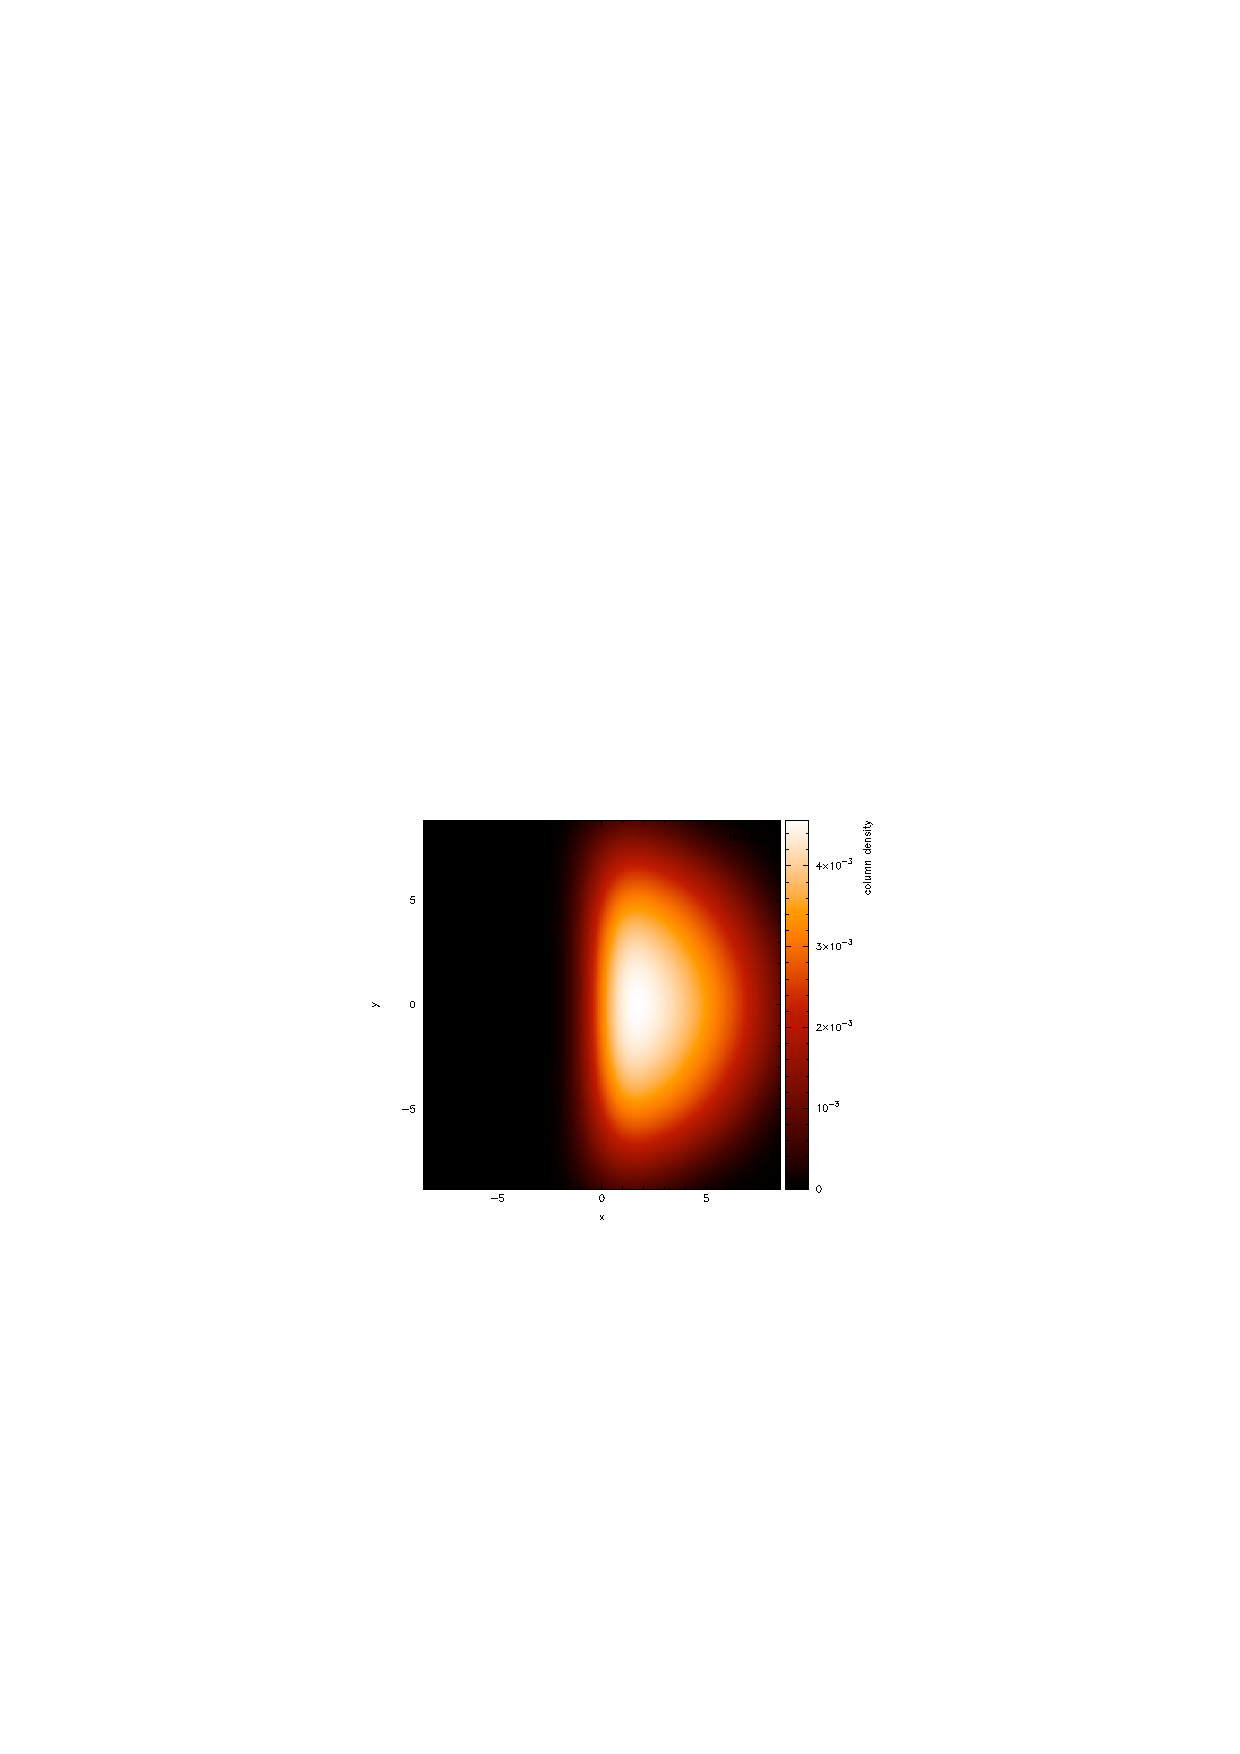
\includegraphics[angle=270,width=0.5\textwidth]{rendersubset.pdf}
\caption{Two examples of multiple dump files plotted on top of each other}
\label{fig:rendersubset}
\end{center}
\end{figure}

When more than one timestep is plotted per page with different markers/colours, an additional legend can be
plotted (turn this on in the le(g)end submenu, or when prompted whilst setting the "plot n steps on top of each other" option). The text for this legend is just the filename by default (if one timestep per file) or just something dull like 'step 1' (if more than one timestep per file). 

To change the legend text, create a file called \verb+legend+ in the working directory, with one label per line. The position of the legend can be changed either manually via the ``legend and title options'' in the p)age submenu, or by positioning the mouse in interactive mode and pressing 'G' (similar keys apply for moving plot titles and the legend for vector plots -- press 'h' in interactive mode for a full list). 

\subsubsection{ Plotting results from multiple files in the same panel}
 See \ref{sec:nstepsontopofeachother}.

\subsubsection{ Plotting more than one dump file on the same page}
 Note that this is slightly different to ``plotting more than one dump file on the same panel''

\subsubsection{ Changing axes settings}
\label{sec:axessettings}
 Axes settings can be changed in the p)age submenu, by choosing ``axes options''. The options are as follows:
\begin{tabular}{rcp{0.8\textwidth}}
-4 & : & same as AXIS=-1, but also draw major tick marks only \\
-3 & : & same as AXIS=-1, but also draw major and minor tick marks; \\
 -2 & : & draw no box, axes or labels; \\
 -1 & : & draw box only; \\
  0 & : & draw box and label it with coordinates; \\
  1 & : & same as AXIS=0, but also draw the coordinate axes (X=0, Y=0); \\
  2 & : & same as AXIS=1, but also draw grid lines at major increments of the coordinates; \\
  10 & : & draw box and label X-axis logarithmically; \\
  20 & : & draw box and label Y-axis logarithmically; \\
  30 & : & draw box and label both axes logarithmically. \\
\end{tabular}

\subsubsection{ Turning axes off}
 Plot axes can be turned off by choosing ``axes options'' in the p)age submenu. See \S\ref{sec:axessettings} for more details. 

\subsubsection{ Turning axes labels off}
 Axes labels and numbering can be turned off via the ``axes options'' option in the p)age submenu. See \S\ref{sec:axessettings} for more details. 

\subsubsection{ Using logarithmic axes labels}
\label{sec:loglabels}
 Logarithmic axes (that is where the quantity plotted is logged) can be set via the ``apply log or inverse transformations'' option in the l)imits submenu or simply by pressing 'l' with the cursor over the desired axis (or the colour bar) in interactive mode. By default the axes labels reads $log(x)$ and the number next to the axis is $-4$ when $x$ is 10$^{-4}$. Logarithmic axes labels (ie. where the label reads $x$ and the number next to the axis is $10^{-4}$ with a logarithmic scale) can be specified by choosing the ``axes options'' option in the p)age submenu and setting the axes option to 10, 20 or 30 as necessary (see \S\ref{sec:axessettings} for more details). 

\subsubsection{ Changing the size of the plotting surface}
\label{sec:papersize}
 The physical size of the viewing surface used for plotting can be changed via the ``change paper size'' option in the p)age submenu. This affects the size of the X-window (if plotted to the screen) and the size of .png or .gif images generated (if plotted to these devices). Several preset options are provided or the paper size in x and y can be explicitly specified (in inches).

\subsubsection{ Dividing the plotting page into panels}
The plotting page can be divided into panels using the ``subdivide page into panels'' option in the p)age submenu. Note that for multiple plots per page (ie. nacross $\times$ ndown $> 1$) a more limited interactive mode applies (basically because the data used for the plots is no longer stored in memory if there is more than one plot on the same page meaning that functionality such as selecting particles must be turned off).

\subsubsection{ Tiling plots with the same $x-$ and $y-$ axes}
\label{sec:tiling}
 Plots with the same $x-$ and $y-$ axes are tiled if the tiling
option from the (p)age options menu (\S\ref{sec:optionspage}) is set. Tiling means that only one axis is shown where multiple plots share the same x or y axis and that the plots are placed as close to each other as possible. For rendered plots a shared colour bar is plotted which spans the full length of the page.

\subsubsection{ Using non-proportional scales for spatial dimensions}
\label{sec:squarexy}
 By default if the x and y axes are both spatial coordinates, the axes are scaled proportionately. This can be changed via the ``spatial dimensions have same scale'' option in the p)age submenu.

\subsubsection{ Using non-square axes on coordinate plots}
 See \S\ref{sec:squarexy}.
 
\subsubsection{ Changing the character height for axes, labels and legends}
 The character height used for axes, labels and legends can be changed via the p)age setup options submenu. Note that the character height is relative to the paper size (which can also be changed -- see \S\ref{sec:papersize}).

\subsubsection{ Using a thicker line width on plots}
 The line width used for axes and text can be changed via the p)age submenu. Note that line width changes are not always obvious when plotting to an interactive device (e.g. an X-window) but influence non-interactive devices strongly. The default line width is 1 which in my experience looks best for pixel-based devices such as .gif and .png (e.g. when making movies). For vector devices such as postscript (e.g. to use in a paper) plots look better with a thicker line width (like 2 or 3). 

\subsubsection{ Changing the foreground and background colours}
\label{sec:pagecolours}
 The background and foreground colour of a plot can be changed vie the ``set foreground/background colours'' option in the p)age submenu.

\subsubsection{ Plotting axes, legends and titles in white even when the labels are plotted in black}
 By default, axes, legends and titles are plotted in the foreground colour (e.g. black). However if the plot itself is also largely black (e.g. when rendering or when lots of particles are plotted) it can be useful to overplot those parts of the axes and labelling which lie on top of the plotting surface in the background colour (e.g. white). A prompt for this is given when setting the ``set foreground/background colours'' option in the p)age submenu. 
 
 The prompt appears as follows:
\begin{verbatim}
---------------- page setup options -------------------
...
 9) set foreground/background colours 
enter option ([0:8], default=0):9
 Enter background colour (by name, e.g. "black") (default=""):white
 Enter foreground colour (by name, e.g. "white") (default=""):black

 Overlaid (that is, drawn inside the plot borders) axis 
 ticks, legend text and titles are by default plotted in 
 the foreground colour [ie. black].

Do you want to plot these in background colour [ie. white] instead ? (default=no):y
\end{verbatim}
 In the above I have selected a background colour of white, a foreground colour of black. Answering yes to the last question means that those parts of the axes which lie on top of the viewing surface (and any labels) will be plotted in white (the background colour) instead of the foreground colour (black). 

\subsection{le(g)end and title options}

\subsubsection{ Adding titles to plots / repositioning titles}
\label{sec:title}
 Plots may be titled individually by creating a file called \verb+titlelist+ in
the current directory, with the title on each line corresponding to the position
of the plot on the page. Thus the title is the same between timesteps unless the
steps are plotted together on the same physical page. Leave blank lines for
plots without titles. For example, creating a file called \verb+titlelist+ in
the current directory, containing the text:
\begin{verbatim}
plot one
plot two
plot three
\end{verbatim}
and positioning the title using the default options, produces the titles shown
on the graph in Figure~\ref{fig:titleexample} (where there are 6 plots on the physical page).

\subsubsection{ Turning off/moving the time legend}
\label{sec:legendoff}
 The position of the time legend can be set interactively by positioning the mouse in the plot window and pressing 'G'. To set the position non-interactively and/or change additional settings such as the justification, use the ``time legend on/off/settings'' option in the le(g)end submenu.

\subsubsection{ Changing the text in the time legend}
\label{sec:timelegendtext}
 The text which appears the time legend (by default this is ``t='') can be changed via the  ``time legend on/off/settings'' option in the le(g)end submenu.

 To rescale the \emph{value} of the time displayed in the time legend (default value is as read from the dump file), see \S\ref{sec:timeunits}.
 
\subsubsection{ Making the legend read ``z='' instead of ``t=''}
 See \ref{sec:timelegendtext}. An option to change the legend text is provided in the  ``time legend on/off/settings'' option in the le(g)end submenu. The numeric value of the time legend is as read into the \verb+time+ array in the read\_data routine. This value can be rescaled by setting a unit for time (see \S\ref{sec:timeunits}). 
  
\subsubsection{ Plotting the time legend on the first row/column of panels / nth panel only}
 An option to plot the time legend on the first row or column of panels or on a single panel only appears in the in the le(g)end submenu.

\subsubsection{ Plotting a length scale on coordinate plots}
 An option to plot a length scale (ie. \verb+|---|+ with a label below it indicating the length) on coordinate plots (ie. plots where both $x-$ and $y-$axes refer to particle coordinates) is provided in the le(g)end submenu.


\subsection{particle plot (o)ptions}
\label{sec:opts}
 The following are tasks which can be achieved via options in the o) menu [particle plot o)ptions].
 
\subsubsection{ Plotting non-gas particles (e.g. ghosts, boundary, sink particles)}
\label{sec:plotparticlesbytype}
 Particles of different types can be turned on or off (ie. plotted or not) using the ``turn on/off particles by type'' option in the particle plot o)ptions submenu. This option also prompts to allow particles of non-SPH types to be
plotted on top of rendered plots (useful for sink or star particles - this option does not apply to SPH particle types).  Turning SPH particle types on or off also determines whether or not they will be used in the rendering calculation (ie. the interpolation to pixels). This particularly applies to ghost particles, where ghost particles will only be used in the rendering if they are turned on via this menu option.

 (The fact that particles of a given type are SPH particles or not is specified by the \verb+UseTypeInRendering+
flags in the set\_labels part of the read\_data file).

\subsubsection{ Plotting non-gas particles on top of rendered plots}
 An option to plot non-SPH particles on top of rendered plots (e.g. sink particles) can be set when turning particle types on/off via the ``turn on/off particles by type'' option in the particle plot o)ptions submenu (see \S\ref{sec:plotparticlesbytype}).

\subsubsection{ Using ghost particles in the rendering}
 See \ref{sec:plotparticlesbytype}.

\subsubsection{ Turn off plotting of gas particles}
 Particles can be turned on or off by type via the ``turn on/off particles by type'' option in the particle plot o)ptions submenu. See \ref{sec:plotparticlesbytype}. 

\subsubsection{ Plotting dark matter particles}
\label{sec:darkmatter}
 To plot dark matter particles (e.g. for the gadget read) the particle type corresponding to dark matter particles must be turned on via the ``turn on/off particles by type'' option in the o) submenu. Turning this option on means that dark matter particles will appear on particle plots. For the gadget data read it is also possible to produce a rendered plot of dark matter column density by defining a smoothing length for dark matter particles via the GSPLASH\_DARKMATTER\_HSOFT environment variable (see \S\ref{sec:gsplash} for details). With this variable set dark matter particles are treated identically to SPH particles and can be rendered as usual (although the only meaningful quantity to render is the mass density).
 
  Note that for simulations using both SPH and dark matter particles, dark matter particles will contribute (incorrectly) to the SPH rendering when the environment variable is set and the plotting of dark matter particles is turned on. Thus to plot just gas column density in this case, dark matter particles must be turned off [via the o) menu option], and similarly to plot just dark matter density if both SPH and dark matter particles are present, SPH particles must be turned off.
 
\subsubsection{ Plotting a column density plot of dark matter/N-body particles}
 See \ref{sec:darkmatter}.

\subsubsection{ Plotting sink particles}
 Sink particles will be plotted on particle plots once turned on via the ``turn on/off particles by type'' option in the particle plot o)ptions submenu. Setting this option also gives a prompt for whether or not to plot sink particles on top of rendered plots (to which the answer should be yes).  See \ref{sec:plotparticlesbytype} for more details.

\subsubsection{ Changing graph markers for each particle type}
 The graph markers used to plot each particle type can be changed via the ``change graph markers for each type'' option in the particle plot o)ptions submenu. The full list of available markers is given in the PGPLOT user guide. 

\subsubsection{ Plotting each particle type in a different colour}
\label{sec:partcolours}
 Each particle type can be plotted in a different colour via the ``set colour for each particle type'' option in the particle plot o)ptions submenu (press `o' from the main menu).

\subsubsection{ Plotting using lines instead of dots (e.g. for energy vs time plots)}
\label{sec:lines}
 An option to plot a line joining all of the points on a plot can be set via the ``plot line joining particles'' option in the particle plot o)ptions submenu. When set, this option plots a line connecting the (gas only) particles
in the order that they appear in the data array. Useful mainly in one dimension or when plotting ascii data, although can give an indication of the relative closeness of the particles in memory and in physical space in higher dimensions. The line colours and styles can be changed.

 To plot the line only with no particles, turn off gas particles using the ``turn on/off particles by type option'' from the o) submenu.
 
\subsubsection{ Plotting multiple lines with different colours/line styles and a legend}

 When multiple timesteps are plotted on the same physical page, the line style can be
changed instead of the colour (this occurs when the change colour option is chosen for multiple steps per page
-- see the ``change plots per page" option in the p)age options submenu [\S\ref{sec:optionspage}]).

\subsubsection{ Joining the dots}
See \ref{sec:lines}.

\subsubsection{ Plotting the size of the smoothing circle around selected particles}
\label{sec:smoothingcircle}
On coordinate plots this option plots a circle of
radius $2h$ around selected particles. 
This is primarily useful in debugging neighbour finding routines. Where only one of the axes is a 
coordinate this function plots an error bar of length $2h$ in either direction is plotted
in the direction of the coordinate axis. See also \S\ref{sec:findingaparticle} for more details.

\subsubsection{ Locating a particular particle in the data set}
\label{sec:findingaparticle}
 The best way to locate a particular particle in the data set is to use the ``plot smoothing circles'' option in the particle plot o)ptions submenu, e.g:
\begin{verbatim}
Please enter your selection now (y axis or option):o5
------------- particle plot options -------------------
 Note that circles of interaction can also be set interactively
Enter number of circles to draw ([0:100], default=0):1
Enter particle number to plot circle around ([1:959], default=1): 868
\end{verbatim}
 then upon plotting a coordinate plot (e.g. x vs y), particle 868 will be plotted with a circle of size $2h$ which makes it easy to distinguish from the other particles. See also \S\ref{sec:smoothingcircle}.

\subsubsection{ Making sure absolutely all particles are plotted}
 By default splash uses ``fast particle plotting'' for particle plots -- this is where the plotting surface is divided into pixels and only a limited number of particles per pixels is plotted (preventing slowdown due to lots of particles being plotted indistinguishably on top of each other). Use of this optimisation can be turned off \emph{just in case} in the particle plot o)ptions submenu, although there should almost never be a good reason to do so.

\subsubsection{ Plotting in different coordinate systems (e.g. cylindrical coordinates)}
\label{sec:geom}
 The coordinates of position and of all vector components can be transformed into non-cartesian coordinate systems using the ``change coordinate system'' option in the particle plot o)ptions submenu. For example, a dump file with columns as follows:
\begin{verbatim}
-------------------------------------------------------
  1) x                     6) log density         
  2) y                     7) v\dx                
  3) z                     8) v\dy                
  4) particle mass         9) v\dz                
  5) h                   
-------------------------------------------------------
 10) multiplot [  4 ]      m) set multiplot 
-------------------------------------------------------
Please enter your selection now (y axis or option):
\end{verbatim}
choosing o), option 7) and choosing cylindrical coordinates then produces;
\begin{verbatim}
 You may choose from a delectable sample of plots 
-------------------------------------------------------
  1) r                     6) log density         
  2) phi                   7) v\dr                
  3) z                     8) v\dphi              
  4) particle mass         9) v\dz                
  5) h                   
-------------------------------------------------------
...
\end{verbatim}
transforming both coordinates and vectors into the chosen coordinate system. Note that rendering is disabled in coordinate systems other than those native to the file (ie. anything non-cartesian for you -- part of the reason for this feature was that I was experimenting with SPH in cylindrical and spherical coordinates where the reverse transformation was necessary). 

 Details of the coordinate transformations are given in \S\ref{sec:coordtransforms}.

 If you have a coordinate system you would like implemented, please email me the details!

\subsubsection{ Plotting vector components in different coordinate systems}
See \S\ref{sec:geom}.

\subsubsection{ Plotting orbital velocities}
See \S\ref{sec:geom}.

\subsubsection{ Plotting against azimuthal angle/cylindrical radius/etc}
See \S\ref{sec:geom}.

\subsubsection{ Plotting the exact solution to common test problems}
\label{sec:exactsolns}
 The following exact solutions are provided
\begin{itemize}
\item Hydrodynamic shock tubes (Riemann problem) -- a full solution is provided for all types of waves propagating in either direction.
\item Spherically-symmetric 3D sedov blast wave problem.
\item Polytropes (with arbitrary $\gamma$)
\item One and two dimensional toy stars. This is a particularly simple test
problem for SPH codes described in \citet{mp04}.
\item Linear wave. This simply plots a sine wave of a specified amplitude, period and
wavelength on the plot specified.
\item MHD shock tubes (tabulated). These are tabulated solutions for 7 specific MHD
shock tube problems.
\item h vs $\rho$. This is the exact solution relating smoothing length and density in
the form $h \propto (m/\rho)^{1/\nu}$ where $\nu$ is the number of spatial dimensions.
\item radial density profiles. For various models commonly used in $N-$body simulations.
\item Exact solution from a file. This option reads in an exact solution from the
filename input by the user, assuming the file contains two columns containing the $x-$ and $y-$ coordinates of
an exact solution to be plotted as a line on the plot specified.
\end{itemize}
Details of the calculation of the exact solutions are given in Appendix~\ref{sec:exact}. An example plot using the Sedov blast wave exact solution is shown in Figure~\ref{fig:sedov}.


\begin{figure}[h]
\begin{center}
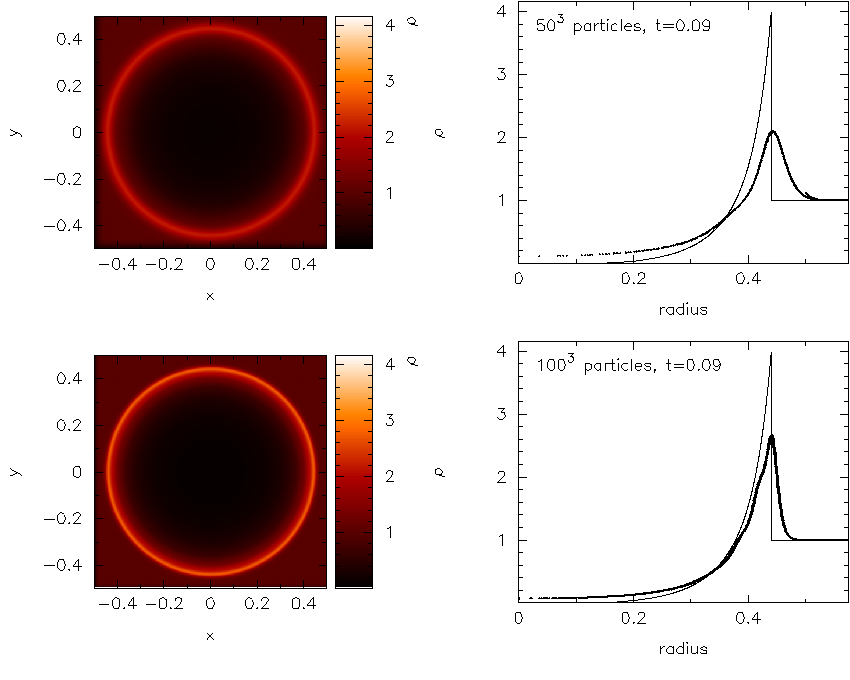
\includegraphics[width=0.5\textwidth]{sedov_example.png}
\caption{Example of a plot utilising the Sedov blast wave exact solution. Taken from Rosswog \& Price (2007).}
\label{fig:sedov}
\end{center}
\end{figure}


\subsubsection{ Plotting an exact solution from a file}
 See \S\ref{sec:exactsolns}. One of the options for exact solution plotting is to read a two column ascii file and plot the results. The filename can be specified by the user and will be saved to the `splash.defaults' file so that the solution will be read and plotted on subsequent invocations of SPLASH.

\subsubsection{ Changing the exact solution line style \& colour}
 The line style and colour of the exact solution line can be changed via the ``exact solution plot options'' option in the o) submenu. This option can also be used to turn on/off calculation of various error norms
together with an inset plot of the residual error on the particles. See
Appendix~\ref{sec:exact} for details of the error norms calculated.

\subsubsection{ Setting the number of points used in an exact solution calculation}
The number of points used in an exact solution calculation can be changed via the ``exact solution plot options'' option in the o) submenu.

\subsubsection{ Plotting an inset plot of residual errors from an exact solution}
 An inset plot of residual errors between the plotted points and an exact solution calculation can be turned on via the ``exact solution plot options'' option in the o) submenu.

\subsection{plot (l)imits}

\subsubsection{ Using plot limits which adapt automatically for each new plot}
\label{sec:adapt}
 Adaptive plot limits can be set using option 1 of the l)imits menu (press 'l' from the main menu, then '1'). Different settings can be applied to coordinate axes and non-coordinate axes. Note that changing plot limits interactively and pressing 's' in interactive mode will change this option back to using fixed limits.

\subsubsection{ Using adaptive plot limits for the colour bar but not for the coordinates}
 Adaptive plot limits can be set individually for coordinate axes and non-coordinate axes (e.g. the colour bar) via the ``use adaptive/fixed limits'' option in the l)imits submenu. See \S\ref{sec:adapt}. 

\subsubsection{ Setting plot limits manually}
 Plot limits can be set manually using option 2) of the l)imits menu (or simply ``l2'' from the main menu). Alternatively you can edit the `splash.limits' file created by a S)ave from the main menu prior to invoking splash (this file simply contains the minimum and maximum limits for each column on consecutive lines).

\subsubsection{ Making plot limits relative to a particular particle}
\label{sec:track}
 Particle tracking limits (ie. where a chosen particle is always at the centre of the plot and limits are set relative to that position) can be set via the ``make xy limits relative to particle'' option in the l)imits menu. Alternatively particle tracking limits can be set interactively by pressing 't' in interactive mode with the cursor over the particle you wish to track. Note that this option only works if particle identities are preserved between timesteps. Also note that, with particle tracking limits set, the radius calculated via the ``calculate extra quantities'' option in the d)ata submenu is calculated relative to the tracked particle.

\subsubsection{ Plotting in a comoving reference frame}
 A co-moving reference frame can be set using the ``make xy limits relative to particle'' option in the l)imits menu. Coordinate limits are then centred on the selected particle for all timesteps, with offsets as input by the user. This
effectively gives the `Lagrangian' perspective. See \S\ref{sec:track} for more details.

\subsubsection{ Setting the origin to correspond to a particular particle}
 See \S\ref{sec:track}.

\subsubsection{ Scaling plot limits by a fixed amount}
 A once-off scaling of the plot limits by a multiplication factor can be applied via the ``zoom in/out'' option in the l)imits menu.

\subsubsection{ Plotting with log axes.}
 Log axes can be set either interactively (by pressing 'l' with the cursor over the desired axis) or manually via the ``apply log or inverse transformations to columns'' option in the l)imits menu. To use logarithmic axes labels as well, see \S\ref{sec:loglabels}.

\subsubsection{ Plotting the square root, inverse or square of a quantity}
 Columns can be logged, inverted, sqrt-ed, squared or any combination of the above via the ``apply log or inverse transformations to columns'' option in the l)imits menu. If you have any additional transformations you would find useful please let me know, as it is straightforward to add more.

\subsubsection{ Resetting limits for all columns}
\label{sec:resetlimits}
 Limits for all columns can be reset to their minimum and maximum values from the current dump file via the ``reset limits for all columns'' option in the l)imits menu. See \S\ref{sec:interactive} for details of resetting plot limits for a particular plot in interactive mode. 

\subsubsection{ Restoring all plot limits to their minimum and maximum values in the current dump file}
See \S\ref{sec:resetlimits}.

\subsection{(r)endering options}
\subsubsection{ Changing the number of pixels in a rendered image}
 The number of pixels in a rendered image can be changed using the r)ender menu, option 1 (or simply type ``r1'' from the main menu). The number set is the number of pixels along the
$x-$axis. The number of pixels along the $y-$axis is determined by the aspect ratio of the plot.

\subsubsection{ Changing the colour scheme}
 The colour scheme used for rendered plots can be changed either by pressing `m' or `M' in interactive mode to cycle through the available schemes or manually by using the ``change colour scheme'' option in the r)ender menu.

 A demonstration of all the colour schemes can be also be invoked from
this menu option. Setting the colour scheme to zero plots only the contours of
the rendered quantity (assuming that plot contours is set to true). The colour
schemes available are shown in Figure~\ref{fig:colourschemes}.
\begin{figure}
\begin{center}
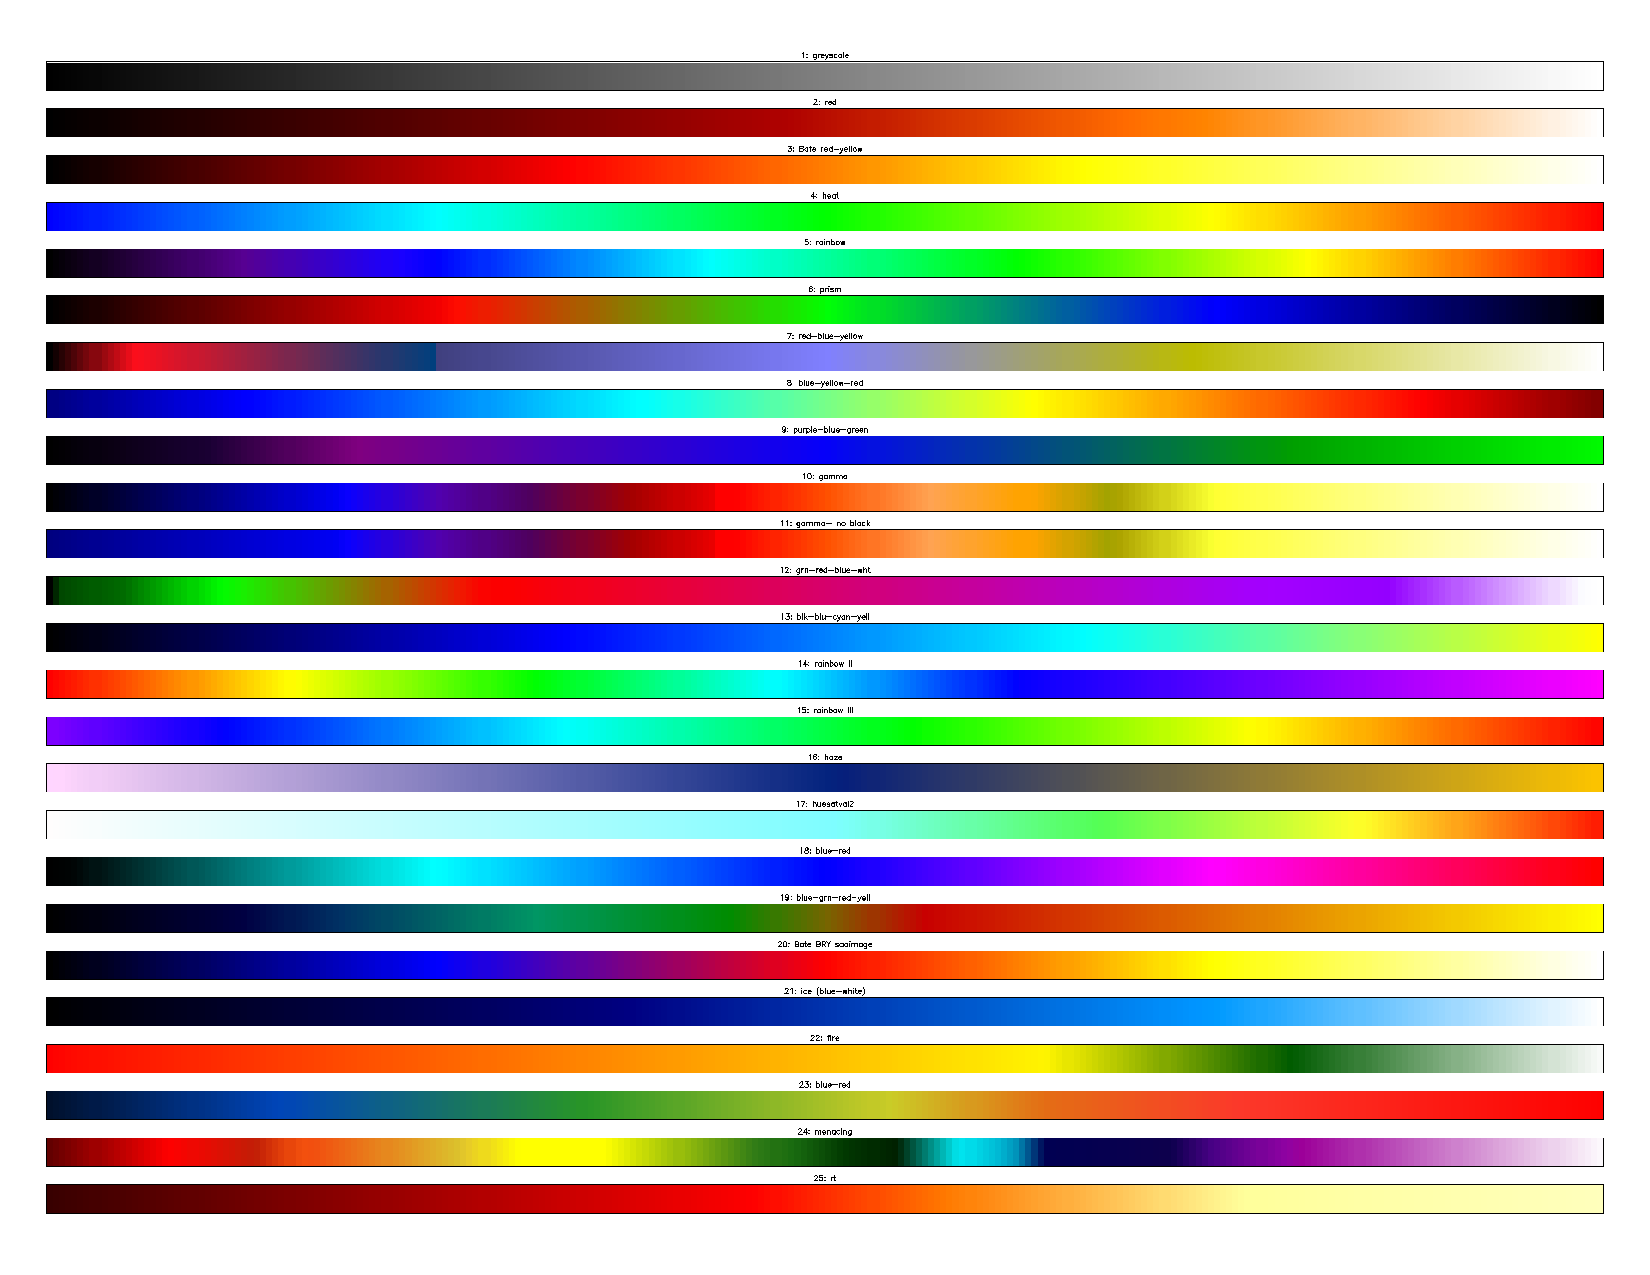
\includegraphics[angle=270,width=\textwidth]{colourschemes.pdf}
%%\begin{turn}{270}\epsfig{file=colourschemes.ps,height=\textwidth}\end{turn}
\caption{SPLASH colour schemes}
\label{fig:colourschemes}
\end{center}
\end{figure}

 User contributed colour schemes are eagerly invited (just send me either: a table of r,g,b colour indices [if you know them] or just an image of a colour bar you wish to reproduce and I will add it).

\subsubsection{ Plotting contours as well as the rendered image}
 Contours of the rendered pixel array can be plotted on top of the rendered plot by setting the ``plot contours'' option from the r)ender menu. To plot contours instead of the rendered image, use the ``change colour scheme'' option from the r)ender menu and choose colour scheme 0 (contours only). 

\subsubsection{ Plotting contours instead of a rendered image}
To plot contours instead of the rendered image, use the ``change colour scheme'' option from the r)ender menu and choose colour scheme 0 (contours only). 

\subsubsection{ Changing the number of contour levels}
 The number of contour levels used whenever contours are drawn can be set via the ``change number of contours'' option in the r)ender menu.

\subsubsection{ Turning the colour bar off/ moving the colour bar label}
 The colour bar can be turned on or off and the style chosen (e.g. horizontal vs vertical) and for the vertical bar, the label moved closer to the bar itself, via the ``colour bar options'' option in the r)ender menu.

\subsubsection{ Using a horizontal colour bar}
 An option to use a horizontal colour bar instead of the default vertical arrangement is given in the ``colour bar options'' option in the r)ender submenu.

\subsubsection{ Using coloured particles instead of rendering to pixels}
\label{sec:colournotrender}
 As a simpler alternative to interpolating to a pixel array, particles can simply be coloured according to the value of a particular quantity by setting the ``use particle colours not pixels'' option in the r)ender menu. With this option set, rendered plots are simply plotted by colouring the particles according to the rendered field. This is somewhat
cruder but can be a good indication of where individual particles might be affecting results.
Note that any colouring of the particles set in interactive mode will be overwritten by use of this option.

\subsubsection{ Using normalised interpolations}
  A normalised interpolation to pixels can be used by setting the ``normalise interpolations'' option from the r)ender menu. In general this leads to smoother rendering but also means that edges and surfaces appear
more prominently (and a bit strange). The general rule-of-thumb I use is therefore to use this option whenever there are no free surfaces in the simulation. Note that in 3D this option only affects cross-section slices (as it is a bit meaningless to normalise a column-integrated or opacity-rendered plot). 

\subsubsection{ Speeding up the rendering on 3D column integrated plots}
 Interpolation on 3D column integrated plots can be made faster by setting the ``use accelerated rendering'' option in the r)ender menu. The reason this is an option is that it makes a small approximation by assuming that each particle lies exactly in the centre of a pixel.  In general this works very well but is not set by default because it can produce funny looking results when the particles are aligned on a regular grid (e.g. as is often the case in initial conditions). Typical speed-ups range from $\times 2$ up to $\times 4$, so it is highly recommended for interactive work.

\subsubsection{ Using density weighted interpolation}
 Density weighted interpolation (where a quantity is plotted times $\rho$) can be turned on in the r)ender menu.

\subsubsection{ Selecting and rendering only a subset of the particles}
 An example of how to render using only a selected subset of the particles was given in \S\ref{sec:rendersubset}.

\subsection{(v)ector plot options}
\label{sec:vectorplots}

\subsubsection{ Changing the number of arrows on vector plots}
 See \S\ref{sec:vecpix}.

\subsubsection{ Changing the number of pixels in vector plots}
\label{sec:vecpix}
 The number of pixels used on vector plots can be changed via the ``change number of pixels'' option in the v)ector menu. This controls the number and average size of the arrows which appear (ie. one arrow is plotted at the centre of each pixel).

\subsubsection{ Changing the size of arrows on vector plots}
 The size of the arrows on vector plots is proportional to the magnitude of the vector quantity at that pixel, where the maximum size is set from the maximum plot limit for the x, y and z components of the vector quantity being plotted such that the longest arrow fills one pixel. These limits can be changed manually via the l)imits menu options. Where these limits are nowhere near the actual values of the vector field, arrows can appear either very big (just a line across the screen) or extremely small (appearing as just dots). Pressing `w' in interactive mode automatically adjusts the arrows to sensible proportions (this is the equivalent of pressing `a' for non-vector quantities). Alternatively pressing `v' (to decrease) or `V' (to increase) can be used to adjust the arrow lengths (the change can be multiplied by 10 or more by first pressing `z' one or more times before pressing 'v' or 'V').

\subsubsection{ Plotting vector arrows in white instead of black or vice-versa}
 Vector arrows are by default plotted using the current foreground colour index (ie. as used for plotting the axes). To plot in the background colour index instead set the ``use background colour for arrows'' option in the v) menu.

\subsubsection{ Turning off the legend for vector plots}
 The legend which appears on vector plots can be turned on or off via the ``vector plot legend settings'' option in the v) menu.

\subsubsection{ Moving the vector plot legend}
 The position of the vector plot legend can be set either interactively by positioning the mouse and pressing 'H' or manually via the ``vector plot legend settings'' option in the v) menu.

\subsubsection{ Plotting stream/fieldlines instead of arrows}
 To plot a vector plot that uses stream/fieldlines instead of arrows, set the ``plot stream/field lines instead of arrows'' option in the v) menu. This option performs a simple integration of the interpolated vector field to get the stream function, the contours of which are then plotted (note that the number of contours can be changed via the ``change number of contours'' option in the r)ender menu). It is generally advantageous to use a larger number of pixels for the vector interpolation (See \S\ref{sec:vecpix}) to get smooth contours.
 
  At present this option works quite well for smooth vector fields but can perform poorly for vector fields with strong gradients.

\subsubsection{ Turning arrow heads off for vector plots}
 Vector plots can be plotted using arrows without heads using the ``turn arrow heads on/off'' option in the v)ector plot options menu.

\subsubsection{ Hiding vector arrows where there are no SPH particles}
 On rendered plots often arrows can appear where there are apparently no SPH particles because the interpolation is performed to all pixels within $2h$ of an SPH particle. Such arrows in regions of few or no particles can be hidden using the ``hide arrows where there are no particles'' option in the v) menu. A threshold number of particles for each pixel can be specified, below which no arrow will be plotted on that pixel.

\subsubsection{ Plotting a vector plot in a cross section slice}
 Vector plots are either in a cross section slice or are column integrated projections depending on the setting of the ``switch between cross section/projection'' option in the x) menu. Setting this to cross section and plotting a vector plot produces a vector plot in a cross section slice.

\subsubsection{ Making all arrow the same length (ie. showing direction only, not magnitude)}
 An option to plot all vector arrows of the same length (instead of the default option where the length of the arrow is proportional to the vector magnitude) can be set from the v) menu.

\subsection{(x) cross section/3D plotting options}

\subsubsection{ Plotting a cross section slice through 3D data}
 When plotting a rendered plot of 3D data, the default option is to plot a column-integrated plot. To change this to a cross section slice, use option 1) in the x) menu (``switch between cross section/projection''). See \S\ref{sec:basic} for examples of how this works. An oblique cross section slice can be set interactively using the 'x' key, see \S\ref{sec:obliquexsec} which works by setting a combination of rotation and a cross section slice position. 

\subsubsection{ Plotting a cross section line through 2D data}
 In 2D, setting the ``switch between cross section/projection'' option in the x) menu to cross section means that rendered plots are in fact a 1D cross section (ie. a line) through 2D data. The position of the line is completely arbitrary (ie. can be set for oblique cross sections as well as straight lines) and is set interactively after the usual $y-$ and $x-$ axis prompts.

\subsubsection{ Rotating the particles}
 An angle of rotation about may be set each axis may be set in the x)sec/rotate submenu using the ``rotation on/off/settings'' option or
interactively (press 'h' in interactive mode to see the exact keystrokes). The position of the origin about which particles are rotated can be set from the ``rotation on/off/settings'' option in the x) menu.
Rotated axes or boxes can be plotted using the ``set axes for rotated/3D plots'' option in the same menu.

Rotations are performed in the order $z-y-x$. This means that the $y-$ rotation angle is an angle about the \emph{new} $y-$axis, defined by the $z$ rotation and similarly for the $x-$ rotation. If you think about it long enough, it makes sense. If in doubt, do it interactively and set the angles in the order $z-y-x$.

\subsubsection{ Setting the origin about which particles are rotated}
 The origin about which particles are rotated and relative to which the radius is calculated when the ``calculate extra quantities'' option is set in the d)ata menu can be changed via the ``rotation on/off/settings'' option in the x) menu.

\subsubsection{ Adding 3D perspective}
\label{sec:3Dperspective}
 3D perspective can be turned on via the ``3D perspective on/off'' option in the x) menu. Prompts for setting the perspective position then appear after the usual prompts for y and x axes, rendering and vector plots, ie. something like the following:
\begin{verbatim}
Please enter your selection now (y axis or option):2
(x axis) (default=1):
 (render) (0=none) ([0:20], default=0):
 (vector plot) (0=none, 7=B, 10=v, 17=J) ([0:17], default=0):
 enter z coordinate of observer (default=1.800):
 enter distance between observer and projection screen ([0.000:], default=0.1800):
 Graphics device/type (? to see list, default /xwin): 
\end{verbatim}
 
  3D perspective is defined by two parameters: a distance to the observer $zobs$ and a distance between the observer and a screen placed in front of the observer, $dscreen$.
The transformation from usual $x$ and $y$ to screen $x'$ and $y'$ is then given by
\begin{eqnarray}
x' & = & x*dscreen/(zobs-z), \nonumber \\
y' & = & y*dscreen/(zobs-z).
\end{eqnarray}
 This means that objects at the screen distance will have unit magnification, objects closer than the
screen will appear larger (points diverge) and objects further away will appear smaller (points
converge). The situation could be beautifully illustrated if I could be bothered drawing a figure. I have found reasonable results with something like a $1/10$ reduction at the typical distance of the object (ie. observer is placed at a distance of $10\times$ object size with distance to screen of $1\times$ object size). SPLASH sets this as default using the z plot limit as the `object size'.

 The position of the 3D observer in $z$ can also be changed in interactive mode using 'u' or 'U' (to move 'up') and 'd' or 'D' (to move 'down'). 

\subsubsection{ Using 3D surface rendering}
 3D surface rendering (turned on using the ``3D surface rendering on/off'' option in the x) menu) performs a ray-trace through the particle data, thus visualising the "last scattering surface". When set, the user is prompted for an "optical depth" before plotting which determines the position of the surface. Only applies to 3D data. When set with cross-section (instead of projection), particles at or below the z value of the slice are used.

The one caveat is that the rendering algorithm needs to use more than 256 colours (for example, if we have a colour map with 256 colours, we need to then have all 256 colours at varying levels of intensity), at present this is implemented by
(optionally) writing the pixel map directly to a .ppm file (called splash\_\#\#\#\#\#.ppm where the number is the number of the current dumpfile) and the approximate version (ie. without the background fade)
is given to the PGPLOT device (e.g. the /xw screen). The .ppm files are uncompressed and therefore somewhat large but can be converted easily to any
other format (e.g. png, ps) using netpbm tools (\url{http://netpbm.sourceforge.net/}) such as
ppmtopng, ppmtops.

 For examples of the 3D surface rendering in SPLASH, have a look at my movies of neutron star mergers at \url{http://www.astro.ex.ac.uk/people/dprice/research/nsmag}.

\subsubsection{ Plotting 3D box / 3D axes}
Rotated axes or boxes can be plotted using the ``set axes for rotated/3D plots'' option in the x) menu.

\subsubsection{ Setting up animation sequences}
\label{sec:animseq}
 Animation sequences can be set via the ``set animation sequence'' option in the x) menu. At present the possible sequences that can be added are:
\begin{verbatim}
 1 : steady zoom on x and y axes                       
 2 : steady rotation                                   
 3 : steady change of limits (e.g. for colour bar)     
 4 : steady movement of 3D observer                    
 5 : sequence of cross section slices through a 3D box 
 6 : steady change of opacity for 3D surface plots
\end{verbatim}
 Up to one sequence of each type can be added (ie. up to 6 in total) with different start and end points (specified in terms of dump file number), with the additional possibility of inserting extra frames between dump files (e.g. to plot a sequence of frames consisting of a changing view of the same dump file). 

 Animation sequences can also be set using `e' in interactive mode. To set a sequence interactively first adjust the plot settings to correspond to the start of the sequence (pressing `s' to save if this is done in interactive mode). Then in interactive mode move to the dump file you want to be the end-point and also adjust the plot settings to correspond to the end-point of your desired sequence (ie. adjust the colour bar limits and/or adjust the rotation angle and/or the x/y limits and/or the 3D observer position and/or the opacity). Then, rather than pressing `s' (which would make these become the default plot settings) press `e' instead, saving these settings as the end-point of the desired animation sequence. This can be done multiple times to set multiple sequences.
 
  Animation sequences set up in this manner are saved to a file called \verb+splash.anim+ either when prompted (if setting sequences non-interactively) or by pressing 'S' from the main menu which then saves both the \verb+splash.limits+ and \verb+splash.anim+ files in addition to the usual \verb+splash.defaults+ file.

\subsubsection{ Plotting a sequence of frames rotating a data set through 360 degrees}
This can be achieved by setting an animation sequence with a steady change of rotation angle. See \S\ref{sec:animseq}.

\subsubsection{ Plotting a `fly-around' of 3D data}
This can be achieved by setting an animation sequence with a steady change of rotation angle. See \S\ref{sec:animseq}.

\subsubsection{ Plotting a flythru of 3D data}
 A sequence of cross section slices progressively deeper into a 3D box or alternatively a steady movement of the 3D observer (on projection plots) can be plotted by setting up an animation sequence. See \S\ref{sec:animseq} for details.

\subsubsection{ Adding a steady zoom sequence to a movie}
 A steady change of $x-$ and $y-$ limits can be added by setting up an animation sequence. See \S\ref{sec:animseq} for details.

\subsubsection{ Adding a steady change of colour bar limits}
 A steady change of limits on the colour bar over one or more dump files for a movie can be implemented by setting up an animation sequence. See \S\ref{sec:animseq} for details.

\subsubsection{ Adding steady movement of the 3D observer}
\label{sec:move3Dobserver}
 The position of the 3D observer can be steadily changed over several dump files (or several frames produced of the same dump file) by setting up an animation sequence.  See \S\ref{sec:animseq} for details.

\subsection{Miscellaneous other useful things}

\subsubsection{ Saving plot settings / plot limits to disk}
 The (s)ave option saves the default options to a file called `splash.defaults' in the
current directory which is read automatically upon the next invocation of
splash. This file uses namelist formatting and may be edited manually prior to  
startup if so desired (this is quite useful for setting multiplots with many plots per
 page).
 
  The (S)ave option writes both the defaults file and also saves the current plot
limits to a file called `splash.limits' which is also read automatically
at startup. If animation sequences have been set (see \S\ref{sec:animseq}), this also saves the `splash.anim' file to disk.

 Typing ``sa'' or ``Sa'' gives a ``save-as'' option, whereby the prefix of files saved by splash can be changed (e.g. using ``sa'' the defaults file can be renamed, whereas using ``Sa'' all files saved by SPLASH are given a new prefix). The prefix to the configuration files which are written by SPLASH can also be changed using the \verb+-p+ option on the command line (the default is ``splash'', ie. ``splash.defaults'', ``splash.limits'' etc).

\subsubsection{ My attempt at in-built help}
The (h)elp option at the moment does nothing particularly useful apart from tell you about menu shortcuts (see \S\ref{sec:menushortcuts}). It seemed like a good idea at the time\ldots

\subsubsection{ Keyboard shortcuts to menu options}
\label{sec:menushortcuts}
Menu options which normally require two keystrokes (e.g. x menu, option 1) can be shortcut to by simply typing the letter and number together at the main menu prompt (so e.g. ``x1'' for x menu, option 1, ``r2'' for render menu, option 2, etc.). This can be quite useful if you are playing around with one particular option a lot.

\subsubsection{ Exiting splash}
 (q)uit, unsurprisingly, quits. Typing a number greater than the number of
data columns also exits the program (e.g. I often simply type 99 to exit).


\section{Advanced plotting examples}

\subsection{Rendered plot of star formation data}
 This is an example using data provided by Paul Clark. The data is from an SPH simulation of star formation in sphNG format. We read the dump file as follows:
\begin{verbatim}
dprice/dustfrag> ssplash omuk162
\end{verbatim}
after which we get output along the lines of:
\begin{verbatim}
...
 reading single dumpfile
>>>>>>>>>>>>>>>>>>>>>>>>>> omuk162 <<<<<<<<<<<<<<<<<<<<<<<<<<
double precision dump
File ID: FHydroRTMHD1
 npart =  11744854
...
\end{verbatim}
and arrive at the main menu:
\begin{verbatim}
 You may choose from a delectable sample of plots 
-------------------------------------------------------
  1) x                                7) v\dx                
  2) y                                8) v\dy                
  3) z                                9) v\dz                
  4) particle mass        10) u                   
  5) h                              11) grad h              
  6) density             
-------------------------------------------------------
 12) multiplot [  4 ]      m) set multiplot 
-------------------------------------------------------
 d(ata) p(age) o(pts) l(imits) le(g)end h(elp)
 r(ender) v(ector) x(sec/rotate) s,S(ave) q(uit)
-------------------------------------------------------
Please enter your selection now (y axis or option):
\end{verbatim}
here we want to plot a rendered plot of column density (density is in column 6), so we type `2' for column 2 (y) as the y axis, `1' for column 1 (x) as the x-axis and at the render prompt `6', for density, ie:
\begin{verbatim}
Please enter your selection now (y axis or option):2
(x axis) (default=1):
 (render) (0=none) ([0:11], default=0):6
 (vector plot) (0=none, 7=v) ([0:7], default=0):0
 Graphics device/type (? to see list, default /xw): /xw
\end{verbatim}
producing the plot shown in Figure~\ref{fig:starpart1} -- somewhat black! The main thing to note is the limits on the colour bar (extending from $0$ to $10^{7}$ on a linear scale) which is the main source of all the blackness. Moving the cursor over the colour bar and pressing `l' for log produces the figure shown on the right hand side --- a vast improvement!
\begin{figure}[h]
\begin{center}
\begin{tabular}{cc}
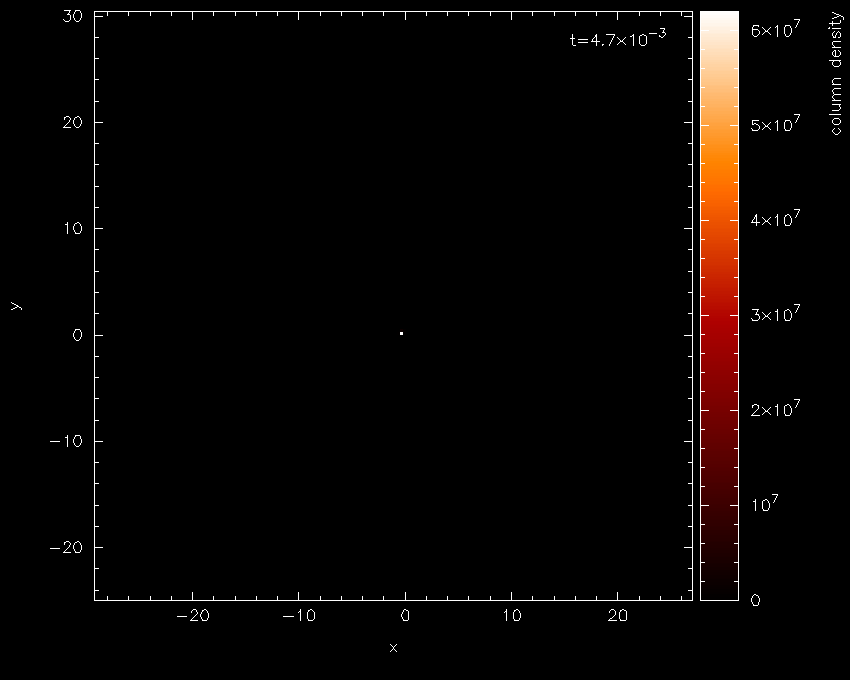
\includegraphics[width=0.5\textwidth]{starpart1.png} &
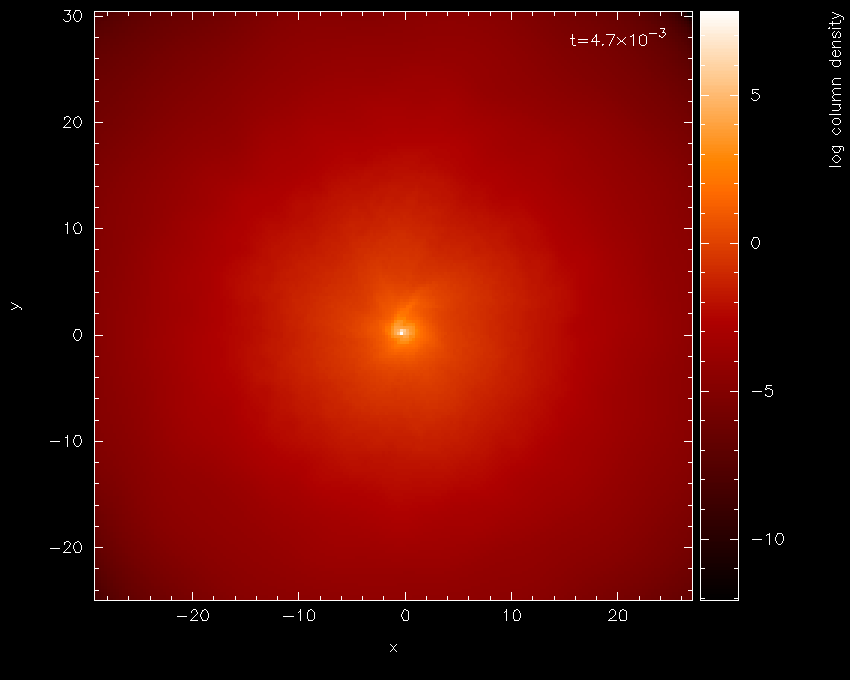
\includegraphics[width=0.5\textwidth]{starpart2.png}
\end{tabular}
\caption{First stage in the star formation figure tutorial: a simple render plot of density (left) and with a log axis after having placed cursor over colour bar and pressed `l' (right)}
\label{fig:starpart1}
\end{center}
\end{figure}
For this visualisation we will eventually want the data in physical units rather than code units. For the sphNG read these units are already specified in the read\_data routine, so all we have to do is turn physical units on. Pressing `q' from interactive mode (that is, with the cursor in the plot window) returns us to the main menu.

 Physical units are turned on from the d)ata menu, as follows:
\begin{verbatim}
Please enter your selection now (y axis or option):d
----------------- data read options -------------------
 0) exit 
 1) read new data /re-read data
 2) change number of timesteps used        (     1 )
 3) plot selected steps only               (  OFF )
 4) buffering of data on/off               (  OFF )
 5) turn calculate extra quantities on/off (  OFF )
 6) use physical units                     (  OFF )
 7) change physical unit settings 
enter option ([0:7], default=0):6
 current settings for conversion to physical units are:
x [cm] = x x  1.000E+17
y [cm] = y x  1.000E+17
z [cm] = z x  1.000E+17
particle mass [g] = particle mass x  1.991E+33
h [cm] = h x  1.000E+17
density [g/cm\u3\d] = density x  1.991E-18
v\dx [cm/s] = v\dx x  3.645E+04
v\dy [cm/s] = v\dy x  3.645E+04
v\dz [cm/s] = v\dz x  3.645E+04
u [erg/g] = u x  1.328E+09
grad h = grad h x  1.000E+00
time = time x 1.69E+00
Use physical units? (default=yes):
\end{verbatim}
returning us to the main menu with labels changed as follows:
\begin{verbatim}
You may choose from a delectable sample of plots 
-------------------------------------------------------
  1) x [cm]                7) v\dx [cm/s]         
  2) y [cm]                8) v\dy [cm/s]         
  3) z [cm]                9) v\dz [cm/s]         
  4) particle mass [g]    10) u [erg/g]           
  5) h [cm]               11) grad h              
  6) log density [g/cm\u3
-------------------------------------------------------
 12) multiplot [  4 ]      m) set multiplot 
-------------------------------------------------------
 d(ata) p(age) o(pts) l(imits) le(g)end h(elp)
 r(ender) v(ector) x(sec/rotate) s,S(ave) q(uit)
-------------------------------------------------------
Please enter your selection now (y axis or option):
\end{verbatim}
at this stage we will save the current settings to file by pressing `s' from the main menu.
\begin{verbatim}
Please enter your selection now (y axis or option):s
 default options saved to file splash.defaults
\end{verbatim}
Actually we would prefer the column labels in AU, but we will come to that later. Replotting the same plot (that is 2, 1, 6, 0, /xw from the main menu) plots the same plot we had before, but with the axes in physical units. Zooming in (using the mouse) on the region of interest and adapting the colour bar limits by moving the mouse over the colour bar and pressing `a' produces the plot shown in the left panel of Figure~\ref{fig:starpart2}. 
\begin{figure}[h]
\begin{center}
\begin{tabular}{cc}
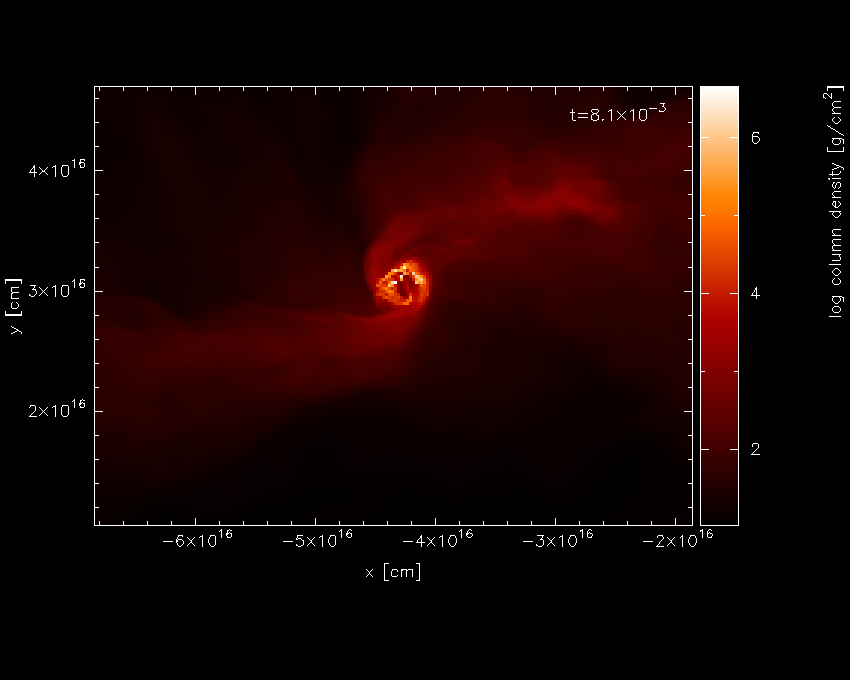
\includegraphics[width=0.5\textwidth]{starpart3.png} &
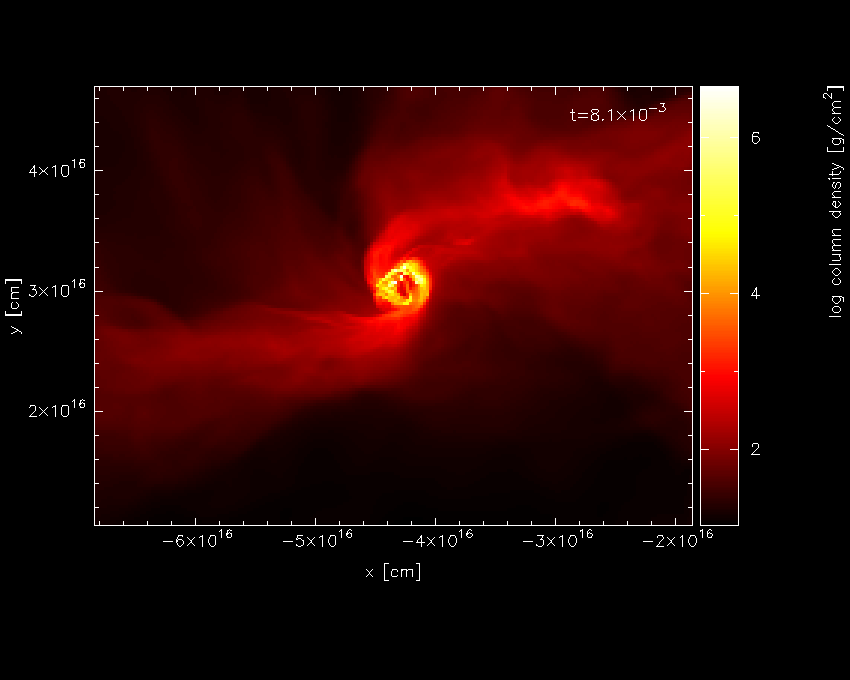
\includegraphics[width=0.5\textwidth]{starpart4.png}
\end{tabular}
\caption{Second stage in the star formation figure tutorial: having applied physical units, zooming in and pressing `a' on the colour bar (left) and having changed the colour scheme (right)}
\label{fig:starpart2}
\end{center}
\end{figure}
 For this kind of plot, the Bate colour scheme looks better -- pressing `m' with the mouse in the plot window changes the colour scheme, producing the plot shown in the right hand panel of Figure~\ref{fig:starpart2}. Pressing `s' in interactive mode (that is, with the mouse in the plot window) saves the current zoom and colour bar settings (but not to disk until you also press `S' from the main menu). Pressing `q' from interactive mode returns to the main menu.
 
 Next we want to turn on the plotting of sink particles (all particle types other than gas are turned off by default). This is done in the o)ptions submenu as follows:
\begin{verbatim}
 Please enter your selection now (y axis or option):o
------------- particle plot options -------------------
 0) exit 
 1) turn on/off particles by type       ( ON, OFF, OFF, OFF )
 2) change graph markers for each type  (  1,  4, 17,  1 )
 3) set colour for each particle type   ( -1, -1, -1, -1 )
 4) plot line joining particles         ( OFF ) 
 5) plot smoothing circles              (   0 ) 
 6) use fast particle plotting          ( ON  ) 
 7) change coordinate systems           (  1 ) 
 8) plot exact solution                 (  0 ) 
 9) exact solution plot options 
enter option ([0:9], default=0):1
 Plot gas particles? (default=yes):
 Plot ghost particles? (default=no):
 Plot sink particles? (default=no):y
 >> Plot sink particles on top of rendered plots? (default=no):y
 Plot unknown/dead particles? (default=no):
\end{verbatim}
 Repeating our previous plot (ie. 2, 1, 6, 0, /xw) produces the plot shown in the left panel of Figure~\ref{fig:starpart3}. 
 \begin{figure}[h]
\begin{center}
\begin{tabular}{cc}
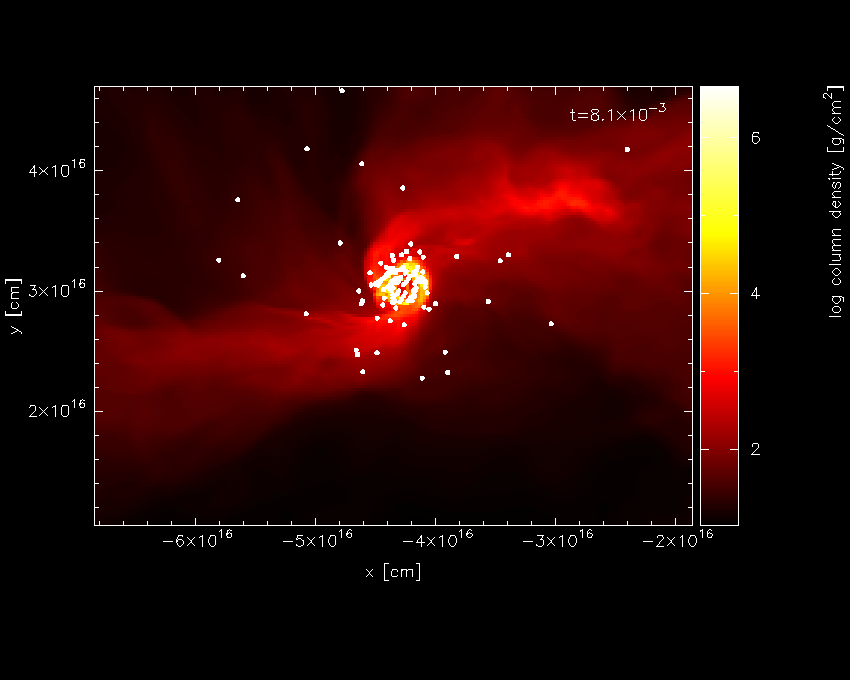
\includegraphics[width=0.5\textwidth]{starpart5.png} &
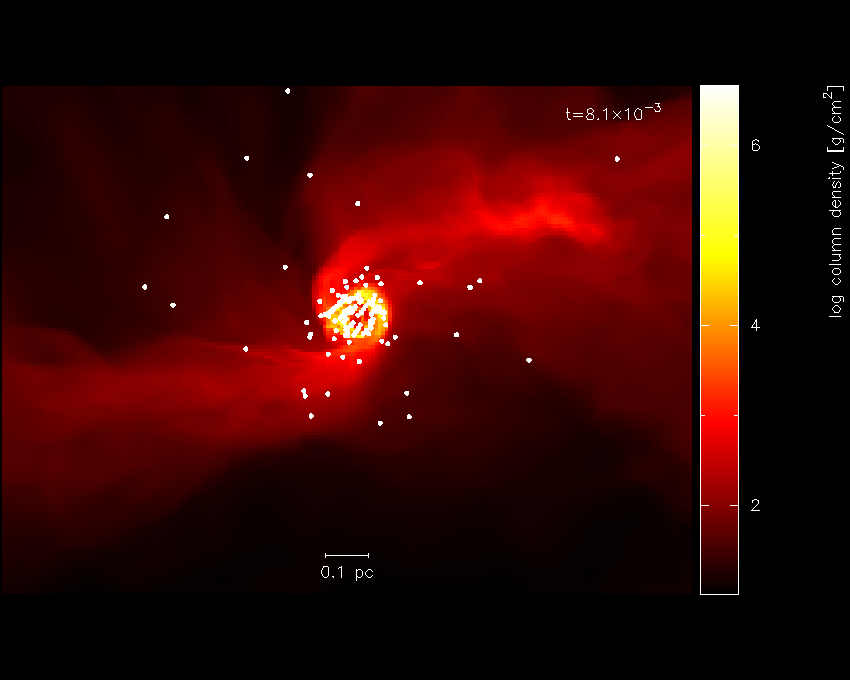
\includegraphics[width=0.5\textwidth]{starpart6.png}
\end{tabular}
\caption{Third stage in the star formation figure tutorial: having turned sink particle plotting on (left) replacing the axes with a scale (right)}
\label{fig:starpart3}
\end{center}
\end{figure}
 The axes in [cm] are kind of ugly, so we could either change this to a sensible unit or plot a scale instead. We will do the latter. The axes can be turned off in the p)age submenu, as follows:
\begin{verbatim}
 Please enter your selection now (y axis or option):p
---------------- page setup options -------------------
...
 2) axes options                      ( 0)
...
enter option ([0:8], default=0):2
  -4 : draw box and major tick marks only;
 -3 : draw box and tick marks (major and minor) only;
 -2 : draw no box, axes or labels;
 -1 : draw box only;
  0 : draw box and label it with coordinates;
  1 : same as AXIS=0, but also draw the coordinate axes (X=0, Y=0);
  2 : same as AXIS=1, but also draw grid lines at major increments of the coordinates;
 10 : draw box and label X-axis logarithmically;
 20 : draw box and label Y-axis logarithmically;
 30 : draw box and label both axes logarithmically.
enter axis option ([-4:30], default=0):-2
   axis =  -2
\end{verbatim}
The option to plot a scale of a particular length is also to be found in the le(g)end menu. We will choose to plot a scale of length 0.1 pc. 
\begin{verbatim}
Please enter your selection now (y axis or option):g
---------------- legend and title options -------------------

 To set the plot titles, create a file called
  'splash.titles' in the working directory, with one title per line

 0) exit 
 1) time legend on/off/settings                ( ON   0.87  1.87  0.00 "t=")
 2) titles on/off/settings                     ( ON   0.20 -0.92  0.00)
 3) legend for multiple steps per page on/off  ( OFF )
 4) plot scale on co-ordinate plots            ( OFF )
 5) legend only on nth panel/first row/column  (  0 )
Enter option ([0:5], default=0):4
 Plot scale on co-ordinate plots? (default=no):y
 Enter length of scale in the current x,y,z units (default=1.000):3.0856e15
 Enter text to appear below scale (e.g. '10 AU') (default=1 unit): 0.1 pc
 Enter horizontal position as fraction of viewport ([0.000:1.000], default=0.5000):
 Enter vertical position in character heights above bottom (default=1.000):
\end{verbatim}
Note that because the x axis units were already in cm, we simply entered the value for 0.1pc in these units. Before plotting again, we should save what we have done so far to disk: Pressing `S' from the main menu saves both the current plot settings \emph{and} the plot limits to disk:
\begin{verbatim}
Please enter your selection now (y axis or option):S
 default options saved to file splash.defaults
 saving plot limits to file splash.limits
\end{verbatim}
Plotting our figure again (2-1-6-0-/xw) produces the plot shown in the right hand panel of Figure~\ref{fig:starpart3}. 

 Nearly there...! To add the finishing touches we want to increase the number of pixels substantially. This is done in the r)ender menu, option 1, for which we can use the shortcut `r1':
\begin{verbatim}
Please enter your selection now (y axis or option):r1
----------------- rendering options -------------------
enter number of pixels along x axis ([1:10000], default=200):1000
\end{verbatim}
then, to plot the figure to file instead of the screen, we simply choose a different PGPLOT device at the prompt:
\begin{verbatim}
Please enter your selection now (y axis or option):2
(x axis) (default=1):
 (render) (0=none) ([0:11], default=6):
 (vector plot) (0=none, 7=v) ([0:7], default=0):
 Graphics device/type (? to see list, default /xw): starpartfinal.gif/gif
\end{verbatim}
producing our final finished Figure shown in Figure~\ref{fig:starfinal}.
\begin{figure}[h!]
\begin{center}
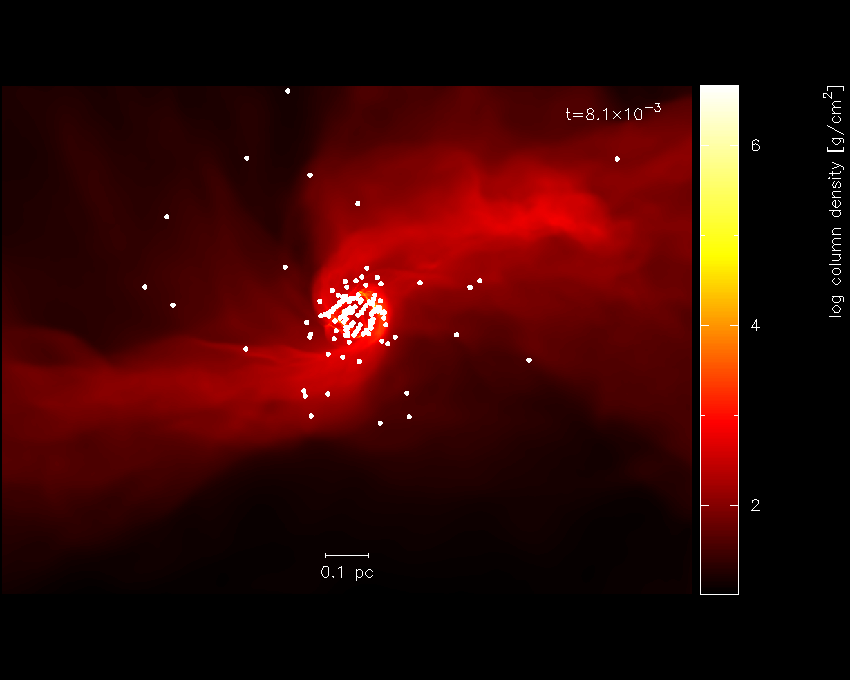
\includegraphics[width=0.5\textwidth]{starpartfinal.png}
\caption{Finished star formation plot}
\label{fig:starfinal}
\end{center}
\end{figure}

 Pressing `S' from the main menu saves all of the settings and plot limits to disk, so invoking splash again will produce the same plot. To produce the same plot on a sequence of dumps, simply put more than one file on the command line and plot to a non-interactive device (see \ref{sec:movies}). Use the postscript devices /ps or /cps (for colour) to make figures suitable for inclusion in a paper.

Other things you may want to do with this plot include:
\begin{itemize}
\item Turn the time legend off. See \S\ref{sec:legendoff}.
\item Change the colour of sink particles. See \S\ref{sec:partcolours}.
\item Change the foreground/background colour of the page. See \S\ref{sec:pagecolours}.
\end{itemize}

\subsection{Multi-panelled figure}
 The following is an example plot taken from \citet{pb07}. Here I will plot a sequence of plots tiled on the same page, so that columns correspond to dumps taken from different runs at the same time and rows correspond to an evolutionary sequence from a given run. The plot uses sphNG data which contains sink particles, so I also want these to appear on the plots and be plotted in white. Basically I want the plots to be plotted such that as much of the plot is taken up by data and very little by axes and the like but still conveying all of the necessary infomation.
 
 We proceed as follows: Firstly, each different run (corresponding in this case to a series of runs with different magnetic field strength) are in different subdirectories with names like \verb+mbossbod_f10.0/+, \verb+mbossbod_f5.0/+, etc. which all contain a sequence of dump files with names like \verb+mbos001+, \verb+mbos002+ etc. To begin the plot, I start by creating a new, empty subdirectory so that the \verb+splash.defaults+ and \verb+splash.limits+ files created by pressing 'S' from the main menu will be in this directory such that running splash from that directory always produces this plot. So:
\begin{verbatim}
dprice% mkdir plot1
dprice% cd plot1
\end{verbatim}
then having decided which dump files from each run to use, I create a text file listing these filenames (with the full relative pathname) in the order in which I will plot them. For example, calling this file (arbitrarily) \verb+filelistplot+, the contents should be something like the following:
\begin{verbatim}
dprice% more filelistplot 
../mbossbod_f20.0/mbos259
../mbossbod_f20.0/mbos263
../mbossbod_f20.0/mbos268
../mbossbod_f20.0/mbos275
../mbossbod_f20.0/mbos294
../mbossbod_f10.0/mbos259
../mbossbod_f10.0/mbos263
../mbossbod_f10.0/mbos268
../mbossbod_f10.0/mbos275
../mbossbod_f10.0/mbos294
../mbossbod_f7.5/mbos259
../mbossbod_f7.5/mbos263
../mbossbod_f7.5/mbos268
...
\end{verbatim}
 Then invoke splash (ssplash for sphNG) with these filenames on the command line:
\begin{verbatim}
ssplash `cat filelistplot`
\end{verbatim}
after which the first dump file should be read, indicated by output along the lines of:
\begin{verbatim}
 reading single dumpfile
>>>>>>>>>>>>>>>>>>>>>>>>>> ../mbossbod_f20.0/mbos259 <<<<<<<<<<<<<<<<<<<<<<<<<<
double precision dump
File ID: SHydroRTMHD1
 npart =  491567
...
\end{verbatim}

An alternative method is to rename the `filelistplot' file \verb+splash.filenames+, from which the filenames will be read if there are none specified on the command line (this feature was implemented as a workaround for a limit to the number of command line arguments on the some compilers).

 The first stage is to get a plot of a single panel looking good. So, from the main menu, we will plot a simple rendering of density and adjust the plot limits until we are happy:
\begin{verbatim}
 You may choose from a delectable sample of plots 
-------------------------------------------------------
  1) x                     6) density             
  2) y                     7) B\dx                
  3) z                     8) B\dy                
  4) particle mass         9) B\dz                
  5) h                   
-------------------------------------------------------
 10) multiplot [  4 ]      m) set multiplot 
-------------------------------------------------------
 d(ata) p(age) o(pts) l(imits) le(g)end h(elp)
 r(ender) v(ector) x(sec/rotate) s,S(ave) q(uit)
-------------------------------------------------------
Please enter your selection now (y axis or option):2
(x axis) (default=1):
 (render) (0=none) ([0:9], default=0):6
 (vector plot) (0=none, 7=B) ([0:7], default=0):
  Graphics device/type (? to see list, default /xw): /xw
\end{verbatim}
which should produce the plot shown in the left hand panel of Figure~\ref{fig:multipart1}. Not much can be seen at first -- just a few white dots. This is mainly a result of the density axis (ie. the colour bar) not being logged. Moving the cursor over the colour bar and pressing `l' results in the plot shown in the right hand panel of Figure~\ref{fig:multipart1}.
\begin{figure}[h]
\begin{center}
\begin{tabular}{cc}
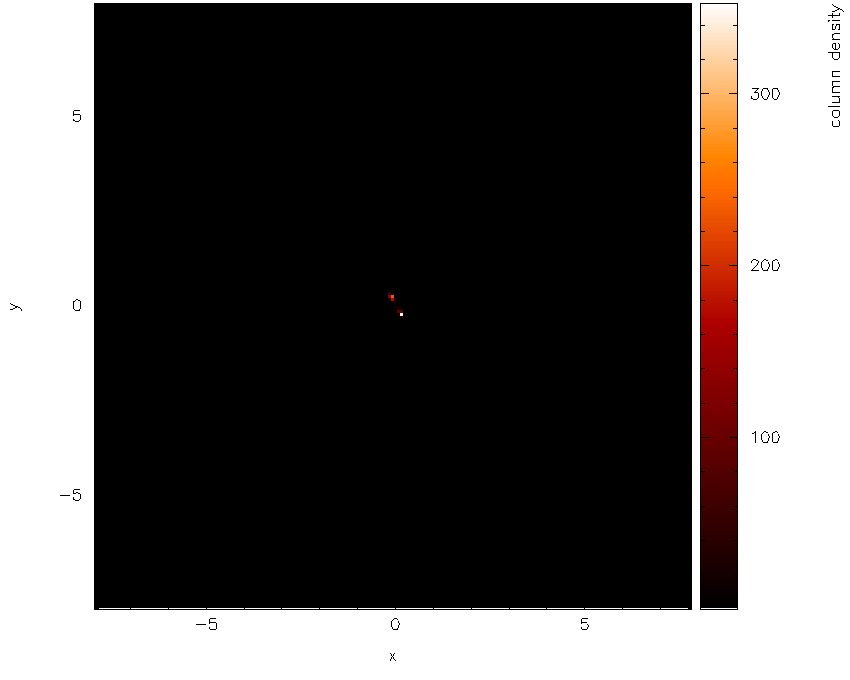
\includegraphics[width=0.5\textwidth]{multipart1.png} &
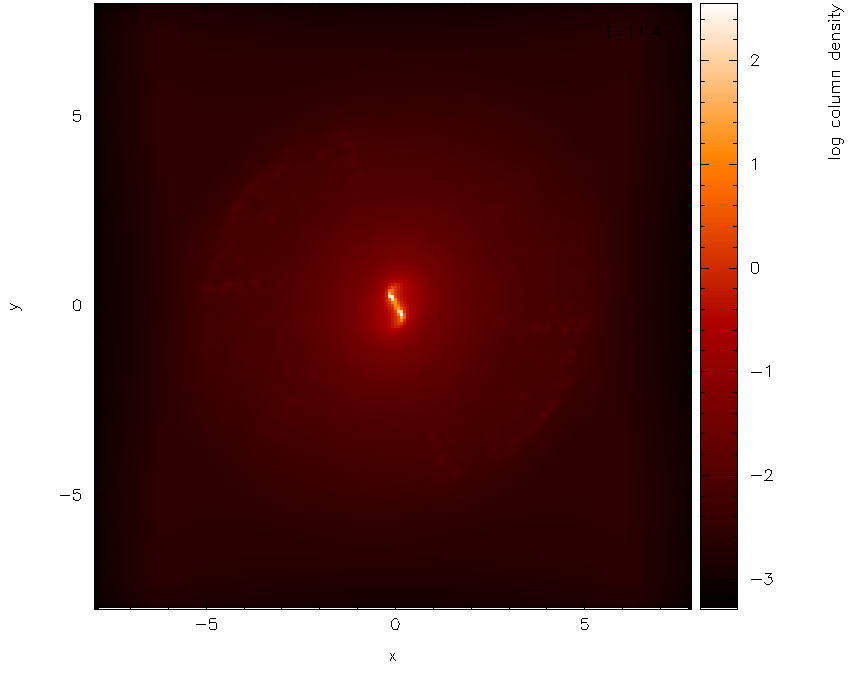
\includegraphics[width=0.5\textwidth]{multipart2.png}
\end{tabular}
\caption{First stage in the multi-panelled figure tutorial: a simple render plot of density (left) and with a log axis after having placed cursor over colour bar and pressed `l' (right)}
\label{fig:multipart1}
\end{center}
\end{figure}

Before we proceed any further, we will first change the axes to be in physical units rather than code units. Pressing `q' in the plot window to exit interactive mode and return to the main menu, and from the d)ata menu, turn the ``use physical units option'' on:
\begin{verbatim}
Please enter your selection now (y axis or option):d
----------------- data read options -------------------
 0) exit 
 1) read new data /re-read data
 2) change number of timesteps used        (     1 )
 3) plot selected steps only               (  OFF )
 4) buffering of data on/off               (  OFF )
 5) turn calculate extra quantities on/off (  OFF )
 6) use physical units                     (  OFF )
 7) change physical unit settings 
enter option ([0:7], default=0):6
 current settings for conversion to physical units are:
x [cm] = x x  1.000E+16
y [cm] = y x  1.000E+16
z [cm] = z x  1.000E+16
particle mass [g] = particle mass x  1.991E+33
h [cm] = h x  1.000E+16
density [g/cm\u3\d] = density x  1.991E-15
B\dx [G] = B\dx x  1.000E+00
B\dy [G] = B\dy x  1.000E+00
B\dz [G] = B\dz x  1.000E+00
time = time x 1.13E-01
Use physical units? (default=yes):yes
\end{verbatim}
 The default transformations to physical units are in this case set in the data read. However it would be nicer in this case to set the x and y axis units to AU (Astronomical Units), rather than cm. From the d)ata menu we proceed as follows:
\begin{verbatim}
enter option ([0:7], default=0):7
 enter column to change units (-2=reset all,-1=quit,0=time) ([-2:9], default=-1):1
 enter x [cm] units (new=old*units) (default=0.1000E+17):668.3893
 enter label amendment (default=[cm]): [AU]
 Apply these units to all coordinates and h? (default=yes):
 Enter unit for 'z' in 3D column integrated plots (default=0.1000E+17):
 Enter label for z integration unit (e.g. [cm]) (default=[cm]):

enter column to change units (-2=reset all,-1=quit,0=time) ([-2:9], default=-1):

save units to file? (default=yes):
 saving plot limits to file splash.units
\end{verbatim}
where in the above I set the multiplicative factor such that the x axis will be in AU and correspondingly changed the units label to `` [AU]'' (note the preceding space). I was also prompted to change the unit for 'z integration' -- this is the length unit added when integrating a quantity through z. Leaving this in cm means that, even though the coordinate axes are in AU, the density (in g/cm$^{3}$) is integrated through z in cm, giving column density in g/cm$^{2}$ (as opposed to g /cm$^{3}$ AU). 

 To save what we have done so far, press `s' from the main menu to save the current settings to the \verb+splash.defaults+ file:
\begin{verbatim}
 Please enter your selection now (y axis or option):s
 default options saved to file splash.defaults
\end{verbatim}

 Having turned physical units on, we replot the same plot (ie. answering 2, 1, 6, 0, /xw to the prompts, as previously). First of all we find simply a white screen. This is a result of the colour bar axis now being wrong. Moving the mouse over the colour bar and pressing `a' (to adapt) results in the plot shown in the left hand panel of Figure~\ref{fig:multipart3}. The plot looks basically identical to the previous plot, except that the axes are now in physical units (x and y are in AU and column density is in g/cm$^{2}$). 

Next, we zoom in to the central region of interest using the mouse -- selecting a region and clicking to zoom in. Pressing `o' centres the plot on the origin and as we zoom in it we also press `a' over the colour bar to readjust the colour bar limits to the max/min on the zoomed-in plot. Finishing with the adjustments (and pressing `s' in the plot window to save the current settings) results in the plot shown in the right hand panel of Figure~\ref{fig:multipart3}.
\begin{figure}[h]
\begin{center}
\begin{tabular}{cc}
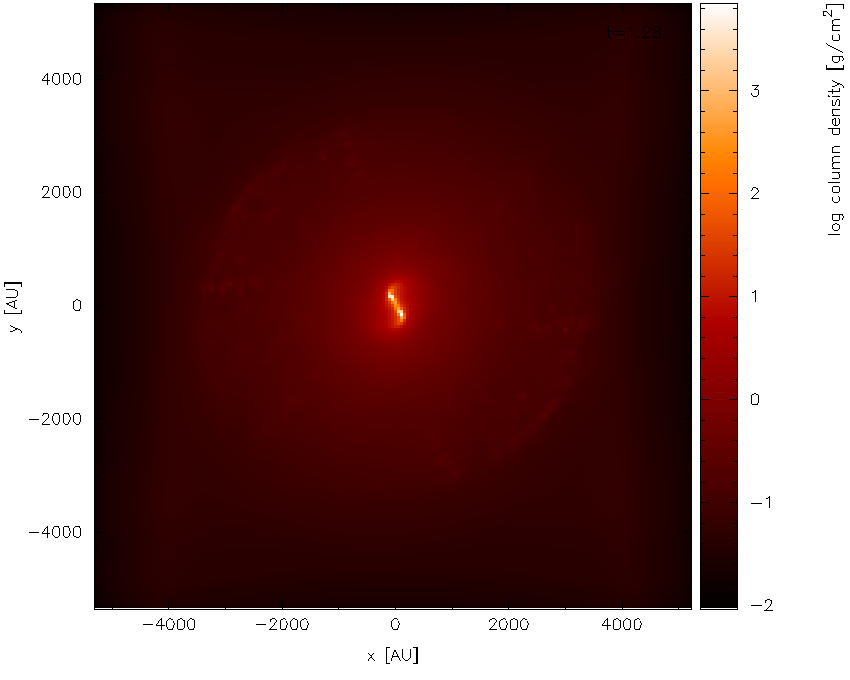
\includegraphics[width=0.5\textwidth]{multipart3.png} &
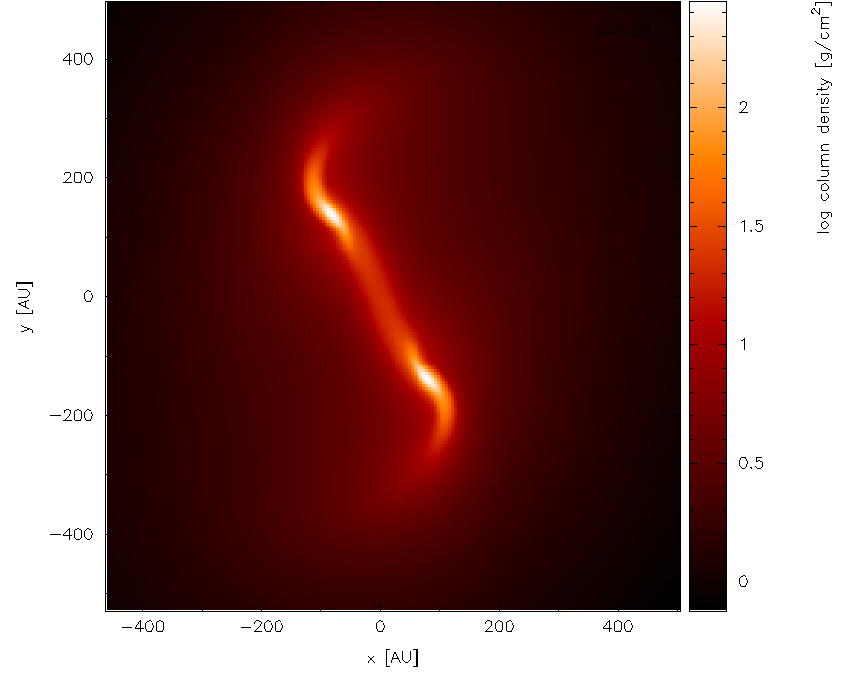
\includegraphics[width=0.5\textwidth]{multipart4.png}
\end{tabular}
\caption{Second stage in the multi-panelled figure tutorial: having changed the axes into physical units (left) and zooming in and adjusting the colour bar (right).}
\label{fig:multipart3}
\end{center}
\end{figure}

\subsection{Surface rendering}
 Here I will give an example of how to use the 3D surface rendering feature starting with a dump file kindly supplied by Giuseppe Lodato from an SPH simulation of a warped accretion disc. First we read the file (in sphNG format, so we use ssplash):
\begin{verbatim}
dprice$ ssplash warp001
\end{verbatim}
after which we reach the main menu:
\begin{verbatim}
 You may choose from a delectable sample of plots 
-------------------------------------------------------
  1) x                     6) density             
  2) y                     7) v\dx                
  3) z                     8) v\dy                
  4) particle mass         9) v\dz                
  5) h                   
-------------------------------------------------------
 10) multiplot [  4 ]      m) set multiplot 
-------------------------------------------------------
 d(ata) p(age) o(pts) l(imits) le(g)end h(elp)
 r(ender) v(ector) x(sec/rotate) s,S(ave) q(uit)
-------------------------------------------------------
Please enter your selection now (y axis or option):
\end{verbatim}
 Firstly we want to plot just a simple render plot of density. Thus we choose:
\begin{verbatim}
 Please enter your selection now (y axis or option):2
(x axis) (default=1):
 (render) (0=none) ([0:9], default=0):6
 (vector plot) (0=none, 7=v) ([0:7], default=0):
 Graphics device/type (? to see list, default /xwin): /xw
\end{verbatim} 
producing the plot shown in the left panel of Figure~\ref{fig:surfpart1} (I have used \verb+/png+ instead of \verb+/xw+ to produce the figures for the userguide). Moving the cursor over the colour bar and pressing `l' to log the colour bar axis produces the Figure in the right panel of Figure~\ref{fig:surfpart1}.
\begin{figure}[h]
\begin{center}
\begin{tabular}{cc}
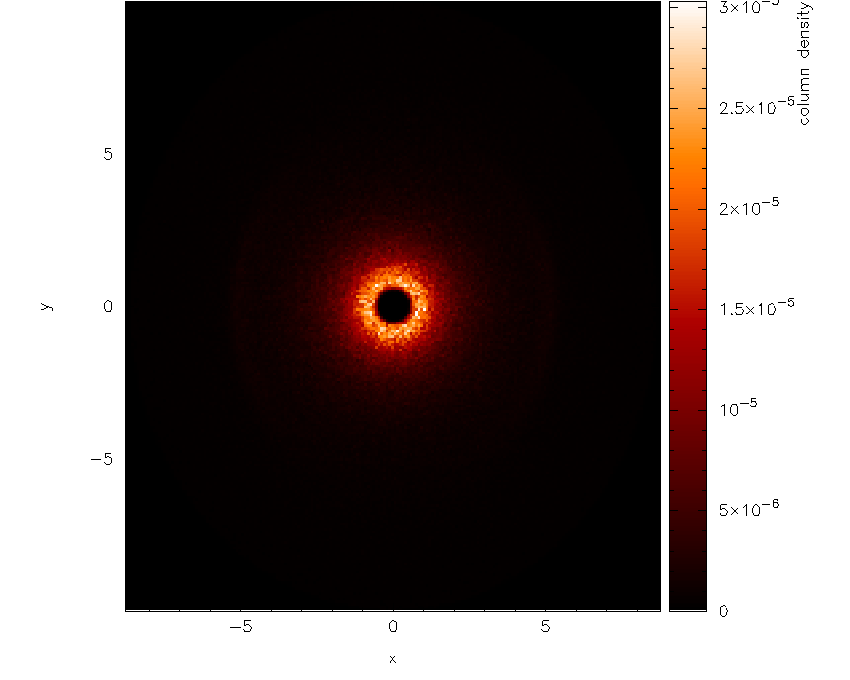
\includegraphics[width=0.5\textwidth]{surfpart1.png} &
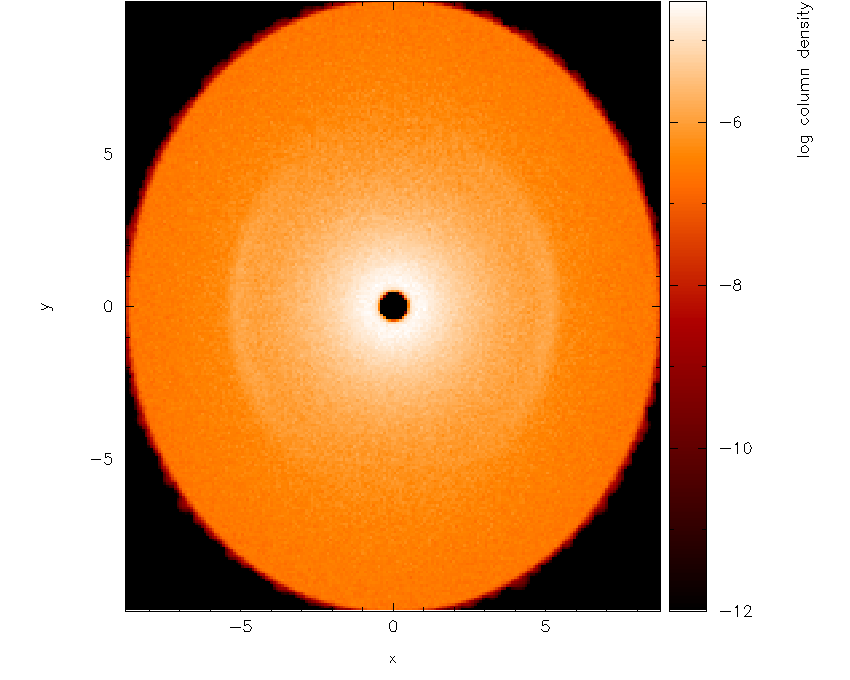
\includegraphics[width=0.5\textwidth]{surfpart2.png}
\end{tabular}
\caption{First stage in the surface rendering tutorial: a simple render plot of density (left) and with a log axis after having placed cursor over colour bar and pressed `l' (right)}
\label{fig:surfpart1}
\end{center}
\end{figure}

The next step is to adjust the viewing angle. Pressing `h' in the plot window brings up the list of keystrokes which can be used to change the angle. Here we want to add a rotation about the $x-$ axis, so we press \verb+{+ three times to change the x angle by -90 degrees and then press \verb+[+ once to increment the angle by a further -15 degrees. The splash output in the terminal reads, amongst other things:
\begin{verbatim}
 rotating particles about z by   0.00
 rotating particles about y by   0.00
 rotating particles about x by 255.00
\end{verbatim}
Then we have the Figure shown in the left panel of Figure~\ref{fig:surfpart2}.
\begin{figure}[h]
\begin{center}
\begin{tabular}{cc}
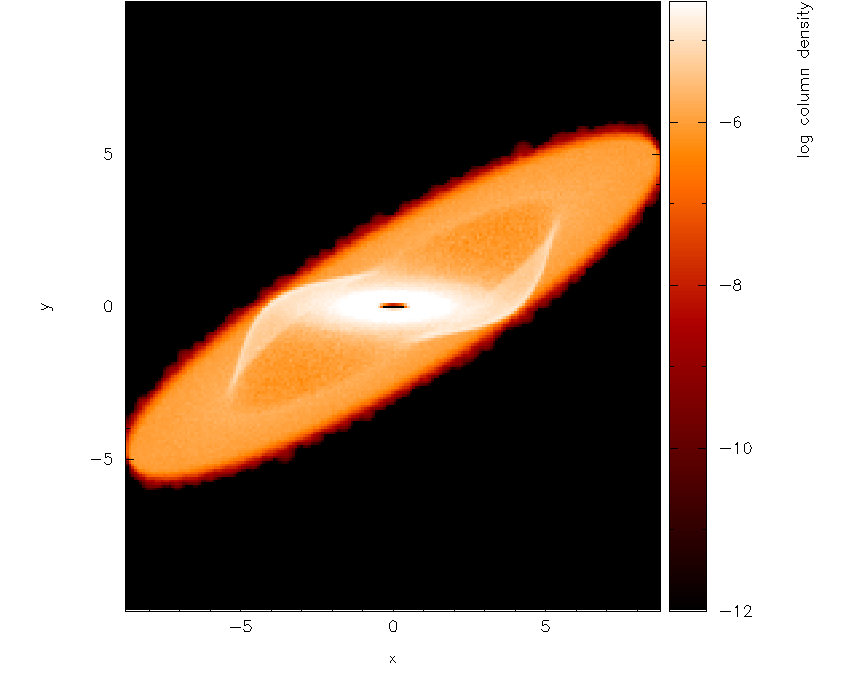
\includegraphics[width=0.5\textwidth]{surfpart3.png} &
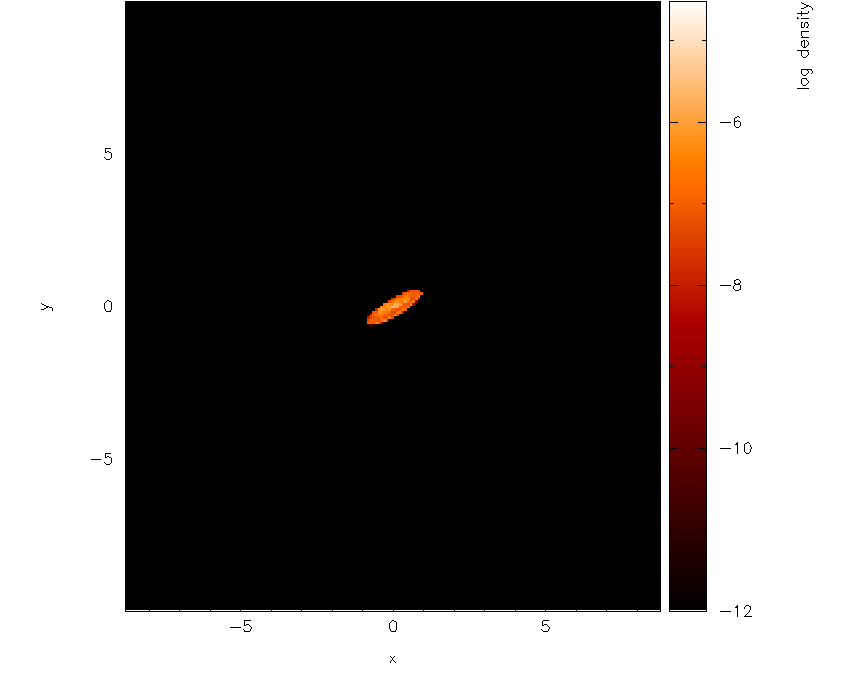
\includegraphics[width=0.5\textwidth]{surfpart4.png}
\end{tabular}
\caption{Second stage in the surface rendering tutorial: after adjusting the rotation angle (left) and with 3D surface rendering turned on (which also turns on 3D perspective) and having adjusted the colour bar limits (right)}
\label{fig:surfpart2}
\end{center}
\end{figure}

 Next, we need to turn the 3D surface rendering on. This cannot be done in interactive mode so we need to exit -- pressing `s' first to save what we have done so far, then 'q' to quit interactive mode. Then, back at the splash main menu, we type x4 for the x)sec/3D plotting options menu, option 4 which is ``3D surface rendering on/off'' with prompts appearing as follows:
\begin{verbatim}
Please enter your selection now (y axis or option):x4
---------- cross section / 3D plotting options --------
Use 3D opacity rendering? (default=yes):y
  also turning on 3D perspective (which must be set for this to work)

 Warning: 3D opacity rendering sends only an approximate version 
 to the PGPLOT device (not corrected for brightness) 

Do you want to write a ppm file in addition to PGPLOT output? (default=yes):y
\end{verbatim}
Now we replot the original plot with the new settings as follows:
\begin{verbatim}
Please enter your selection now (y axis or option):2
(x axis) (default=1):
 (render) (0=none) ([0:9], default=6):
 (vector plot) (0=none, 7=v) ([0:7], default=0):
 enter z coordinate of observer (default=53.58):
 enter distance between observer and projection screen ([0.000:], default=5.358):
 using current h and pmass limits to calculate kappa (cross section/unit mass)
 min h =  0.1197254  min particle mass =  3.812551E-11
 [ kappa = pi*h_min**2/(particle_mass*n_smoothing_lengths) ]
enter approximate surface depth (number of smoothing lengths): ([0.000:], default=2.000):
 kappa (particle cross section per unit mass) =  1.2369025E+9
 Graphics device/type (? to see list, default /xwin): 
\end{verbatim}
Note that several new prompts appear -- for the moment I have just used the default answers by pressing return. The first result is rather frightening : just a black image with a black colour bar! This is because the limits we set for column density are several orders of magnitude away from the limits on density. Moving the cursor over the colour bar and pressing `a' to adapt the limits produces the plot shown in the right panel of Figure~\ref{fig:surfpart2}.

Note that the plot suddenly appears much smaller -- this is a consequence of the 3D perspective settings. Moving the cursor into the plot window and pressing `a' adapts the plot limits. After also clicking on the colour bar and adjusting the colour bar limits, we arrive at the plot shown in the left panel of Figure~\ref{fig:surfpart3}.
\begin{figure}[h]
\begin{center}
\begin{tabular}{cc}
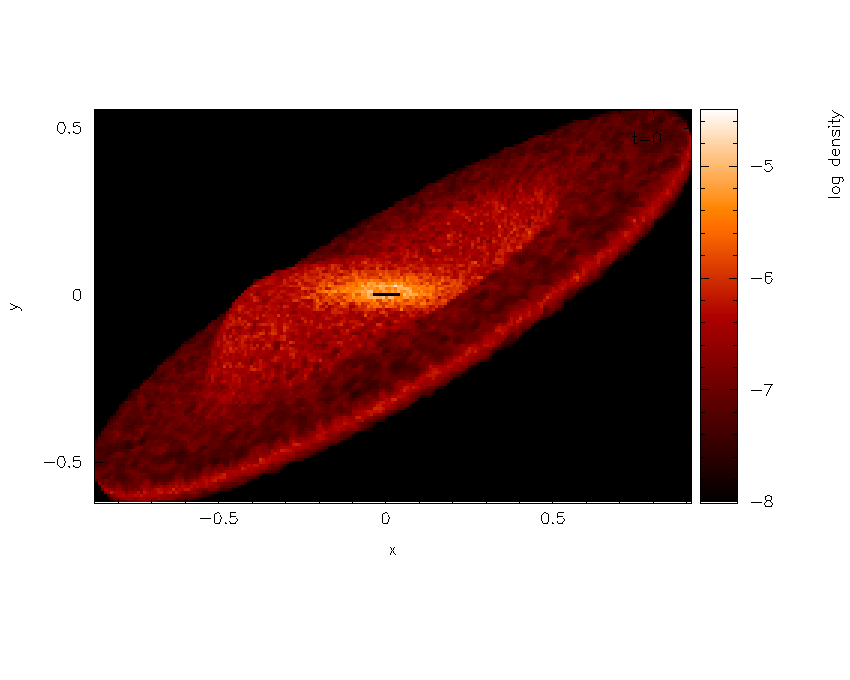
\includegraphics[width=0.5\textwidth]{surfpart5.png} &
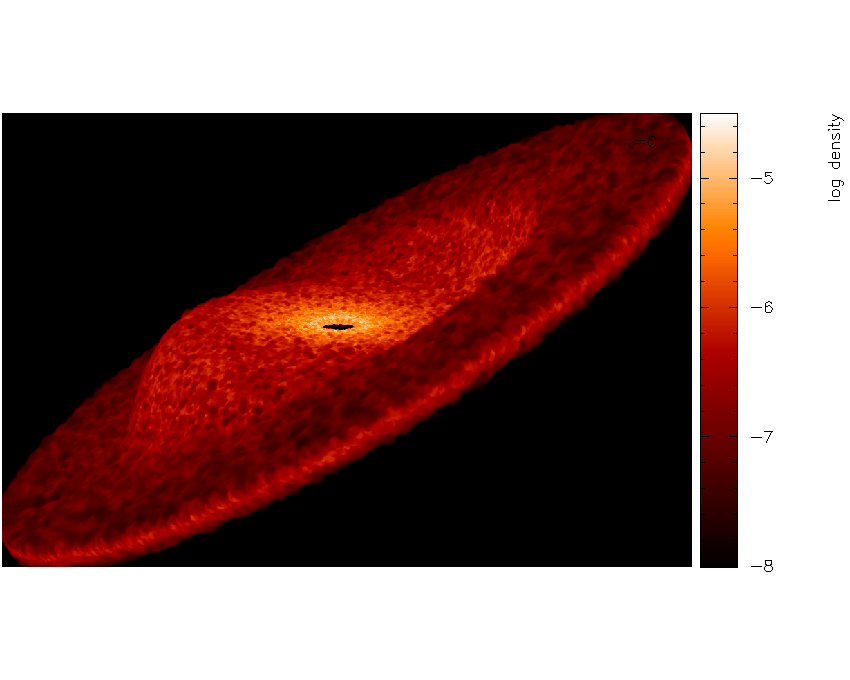
\includegraphics[width=0.5\textwidth]{surfpart6.png}
\end{tabular}
\caption{Third stage in the surface rendering tutorial: after adjusting the xy and colour bar limits interactively (left) and increasing the number of pixels and having turned the axes off (right)}
\label{fig:surfpart3}
\end{center}
\end{figure}

 Now that we are nearly there, to add the finishing touches we need to i) increase the number of pixels in the image and ii) turn the axes off, since they are no longer meaningful with 3D perspective set. The number of pixels can be increased by returning to the splash main menu (pressing `s' in interactive mode before doing so to save what we have done so far), then typing `r1' for render menu, option 1:
\begin{verbatim}
Please enter your selection now (y axis or option):r1
----------------- rendering options -------------------
enter number of pixels along x axis ([1:10000], default=200):1000
\end{verbatim}
Next, we turn the axes off using the p)age submenu:
\begin{verbatim}
Please enter your selection now (y axis or option):p2
---------------- page setup options -------------------
 -4 : draw box and major tick marks only;
 -3 : draw box and tick marks (major and minor) only;
 -2 : draw no box, axes or labels;
 -1 : draw box only;
  0 : draw box and label it with coordinates;
  1 : same as AXIS=0, but also draw the coordinate axes (X=0, Y=0);
  2 : same as AXIS=1, but also draw grid lines at major increments of the coordinates;
 10 : draw box and label X-axis logarithmically;
 20 : draw box and label Y-axis logarithmically;
 30 : draw box and label both axes logarithmically.
enter axis option ([-4:30], default=0):-2
  axis =  -2
\end{verbatim}
 Plotting the same plot again now results in the plot shown in the right panel of Figure~\ref{fig:surfpart3}.

Finally we will also set the background colour to black, adjust the opacity and move the time legend. 
Notice that in the right panel of Figure~\ref{fig:surfpart3} the surface looks quite blotchy. This is an indication that the surface is too shallow (that is we are only seeing particles on the very top). Thus we will adjust the opacity for a slightly deeper plot. We proceed as follows: Exiting interactive mode (pressing `s' then `q' in the plot window), we first set the foreground and background colours in the p)age submenu:
\begin{verbatim}
Please enter your selection now (y axis or option):p8
---------------- page setup options -------------------
Enter background colour (by name, e.g. "black") (default=):black
 Enter foreground colour (by name, e.g. "white") (default=):white
 Do you want to plot axes and overlaid text in background colour (default is foreground) ? (default=no):
\end{verbatim}
Now, replotting the same plot again, but this time adjusting the opacity at the prompt:
\begin{verbatim}
enter approximate surface depth (number of smoothing lengths): ([0.000:], default=2.000):200.0
\end{verbatim}
 Finally, moving the time legend by positioning the cursor and pressing 'G' and zooming out slightly by pressing `-' once, we arrive at our finished figure (or movie frame) shown in Figure~\ref{fig:surfpartfinal}. Pressing `s' in interactive mode saves the settings, then pressing `q' returns to the splash main menu. To save the settings to disk, press `S' from the main menu to save both the \verb+splash.defaults+ file and the \verb+splash.limits+ file.
\begin{figure}[h!]
\begin{center}
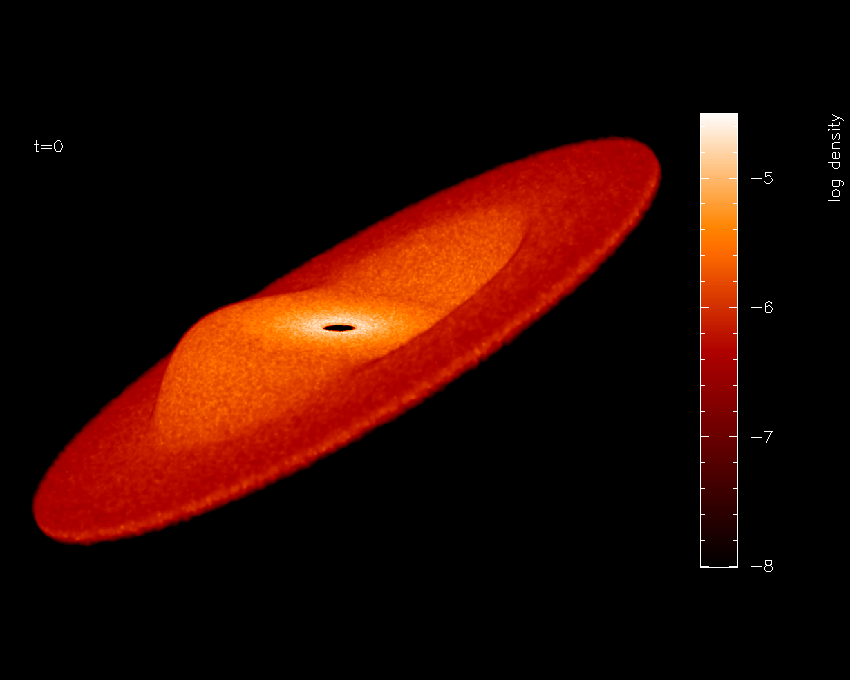
\includegraphics[width=0.5\textwidth]{surfpartfinal.png}
\caption{Finished surface-rendered plot}
\label{fig:surfpartfinal}
\end{center}
\end{figure}
 
  To create a sequence of images with these settings, then simply invoke splash again with multiple files:
\begin{verbatim}
ssplash warp???
\end{verbatim}
then plotting the same plot as previously to a non-interactive device will cycle through all dump files producing a sequence of plots with names like \verb+pgplot.png+, \verb+pgplot.png_2+ etc. (see \S\ref{sec:fixpgplotnames} for details of how to fix the file naming scheme).

\subsection{Using asplash to plot energy vs time plots}
 asplash (that is, the compilation of splash which reads ascii files) can also be used for non-SPH data. For example I often use it to plot the contents of the .ev file my SPH code dumps monitoring quantities like energy and angular momentum at every timestep. A shortcut way of setting options appropriate to reading such files (e.g. plotting lines instead of dots, plotting all files on the same page) is implemented by adding the ``-e'' option to the command line: e.g.
\begin{verbatim}
asplash -e file1.ev file2.ev file3.ev
\end{verbatim}
also, using the -e option on the command line means that any modification to the preset options /limits are saved to files called \verb+evsplash.defaults+ and \verb+evsplash.limits+ instead of the usual \verb+splash.defaults+ and \verb+splash.limits+. This means the defaults for this type of plot are saved separately to those for ``normal'' plots of SPH data.

\subsection{Powerspectrum of 1D data}
 In one dimension an extra plot item appears
in the data menu which takes a power spectrum (in space) of a particular
variable defined on the particles. Upon selection the user is prompted for
various settings before plotting the power spectrum. For data defined on
irregularly distributed particles, there are two methods for taking the power
spectrum: Either to interpolate to an even grid and use a Fourier
transform or to use a method for calculating a periodogram of
irregularly sampled data which can have significant advantages over
interpolation. Algorithms for both of these methods have been
implemented. For the first, the SPH data is interpolated to a one dimensional
grid using the kernel before calculating the (slow!) fourier
transform. The second method computes a Lomb/Scargle periodogram as described in \citet{numericalrecipes}. 

 It should be stressed, however, that \emph{neither} of the subroutines for
calculating the power spectrum is particularly fast and have \emph{only} been included as a preliminary feature since I have used them once or twice in one dimensional simulations where speed is not an issue. The algorithms are fairly simple to extend to multidimensional
data, although faster implementations would be needed (such as a Fast
Fourier Transform routine).


\section{Other useful information}

\subsection{Fixing the PGPLOT file naming system} 
\label{sec:fixpgplotnames}

When you run splash to make a series of plots it generate files with names..
\begin{verbatim}
pgplot.gif
pgplot.gif_1
pgplot.gif_2
...
pgplot.gif_10
pgplot.gif_11
pgplot.gif_12
..
pgplot.gif_200
pgplot.gif_201
\end{verbatim}
The annoying thing is that the numeric indices on these files are out of order and, when using
standard programs to make animations, results in frames out of sequence.

 The problem is related to PGPLOT file naming conventions. The fix is that, included in the splash/scripts directory is a script called 'fixpgplotnames.bash'. If you run this in the directory where your files are located, ie.
\begin{verbatim}
cd mydir
~/splash/scripts/fixpgplotnames.bash
\end{verbatim}
will rename all of the files sensibly. If you run it with a number as the argument
\begin{verbatim}
~/splash/scripts/fixpgplotnames.bash 10
\end{verbatim}
it will rename filenames adding 10 to the number (actually 11 because it starts from 1). This is
useful if you run splash multiple times to get different parts of an animation. 

\subsection{Reading/processing data into images without having to answer prompts}
\label{sec:batchmode}
 The simplest way of running SPLASH
non-interactively is to write a small shell script which runs SPLASH
and answers the prompts appropriately. Something like the following should work:
\begin{verbatim}
#!/usr/bin/tcsh
cd plot
splash myrun* << ENDINPUT
2
1
8
0
mypostcript.ps/ps
q
ENDINPUT
\end{verbatim}
which would plot the data in columns 2 and 1 and render the data in column 8 with
output to file \verb+mypostscript.ps+.

\subsection{Making frames across multiple processors}
 Making identical plots of a series of dump files for a movie is a task which can inherently be done in parallel. Included in the splash/scripts directory is a perl wrapper for splash (``\verb+splash_parallel.pl+'') which distributes multiple instances of splash across multiple machines, either via ssh or using Apple's xgrid, with a common input file as described in \S\ref{sec:batchmode}. The limitation to this is that you need to have a disk which can be mounted from all client machines (ie. they can read the data files) and preferably with password-less access (e.g. using an ssh key-exchange or Kerberos authentication). The script itself may need some slight adjustment for your particular system.
 
However, with large datasets often the slowest part of the rendering process can be reading the data file. A good way of crippling a system is therefore to set 100 jobs going which all decide to read a large data file from disk at the same time. To avoid this the script allows the user to set a delay between launching jobs (preferably slightly longer than the length of time it takes to read a single dump file), but some care is needed to avoid disaster. You have been warned! 

\subsection{What about boundaries? How does the rendering work near a boundary?}
 Usual practise in SPH simulations near boundaries is
to introduce ghost particles which mirror the real particles. SPLASH does not
explicitly setup any ghost particles but will use any that are present in the data
(see next question for how to specify multiple particle types). Additional particle types contribute
to the rendering calculations but not to the determination of the plot limits. Note,
however, that SPLASH does \emph{not} set up ghost particles itself, as this may depend
on the type and location of the boundary. Thus if your simulation uses ghost particle
boundaries, the ghost particles should be dumped alongside the gas particles in the
output file so that their positions, masses, densities and smoothing lengths can be
read into SPLASH and used to render the image appropriately.

\subsection{How does splash handle multiple particle types?}
SPLASH can handle up to 6 different particle types. These can be turned on and off in the particle plot
o)ptions menu (\S\ref{sec:opts}). These types are be specified in the set\_labels part of the read\_data
routine, which contains some lines of code along the lines of:
\begin{verbatim}
ntypes = 3
labeltype(1) = 'gas'
labeltype(2) = 'ghost'
labeltype(3) = 'sink'
UseTypeInRenderings(1) = .true.
UseTypeInRenderings(2) = .true.
UseTypeInRenderings(3) = .false.
\end{verbatim}
which says that there are 3 particle types, with names as given, and that types 1 and 2 are SPH particles and
should be used in the rendering where appropriate (ie. only when plotting of this type is turned on in the
o)pts menu). Particle types which are to be used in renderings should have masses, densities and smoothing
lengths read. Non-SPH particle types (e.g. sink particles) can be optionally plotted on top of rendered plots.

\subsection{Using special characters in the plot labels}
 Several of the examples shown in this manual use special characters (such as
the $\int$ character) in the plot labels. The PGPLOT user guide explains how to do
this, but the basic idea is that PGPLOT uses escape sequences to plot special
characters. For example to plot the greek letter $\rho$ we would use
\begin{verbatim}
label = 'this would print the greek letter \gr'
\end{verbatim}
where \verb+\gr+ is the PGPLOT escape sequence for $\rho$. For other
characters the escape sequence is given by a number. For example for the integral 
\begin{equation}
\int v_x \mathrm{dx}
\end{equation}
we would use
\begin{verbatim}
label = '\(2268) v\d x \u dx'
\end{verbatim}
where \verb+\(2268)+ is the escape sequence for the integral sign. The
\verb+\d+ indicates that what follows should be printed as subscript and
\verb+\u+ correspondingly indicates a return to normal script (or from normal script to
superscript). All of the escape sequences for special characters are listed in
the appendix to the PGPLOT user guide.
\begin{quote}
 WARNING: Note that the use of escape characters can be compiler dependent and
 may not therefore work on all compilers (for example the intel compiler needs
 the -nbs flag).
\end{quote}

\subsection{Making movies}
See \S\ref{sec:movies} and the online FAQ (\url{http://www.astro.ex.ac.uk/people/dprice/splash/faqs.html}).

\subsection{Outputting the raw pixel map to a file}
 The actual pixel map rendered to the graphics device (ie. when a quantity is rendered to pixels, not for particle plots) can be output directly to a file, or series of files by using the \verb+-o+ command line option when you invoke SPLASH. Invoking SPLASH with \verb+-o+ produces a list of currently implemented formats (at the moment these are an ascii dump file and ppm format). This is useful if you need to compare the image to the output from another code (e.g. using a different visualisation tool) or if you wish to have a ``raw'' rendering, that is without annotation on the plots, but which (in the ppm case) uses more colours. The files are given default names such as ``splash\_00001.dat'' or ``splash\_00001.ppm'' where the number corresponds to the frame number as would be rendered to the PGPLOT graphics device.

\section{User contributions / Wishlist for future improvements}
 Please contribute!! Any user contributions and/or suggestions would be greatly
appreciated. The following in particular would be very useful:
\begin{itemize}
\item Suggestions, suggestions, suggestions! I am always on the lookout for what users other than me actually want to do.
\item Bugs!
\item Pretty pictures! If you happen to plot some of your data and spend the
next several minutes marvelling at how astoundingly beautiful it all looks, please send
me a copy (either ps, gif or a movie) to add to the gallery and a few lines
describing the simulation.
\end{itemize}
If you are *really* keen, you may also like to consider:
\begin{itemize}
\item Exact solutions for your favourite test problem(s). Even just an analytic description which I can write the code for, or a subroutine if you're brave.
\item Data analysis tools (e.g. fourier transforms / statistical analysis /
algorithms for finding binary stars etc) which could be incorporated.
\item New visualisation techniques (e.g. an isosurfacing routine for SPH, 3D stream line tracing).
\item More colour schemes (simply email me a table of the rgb colour indices, or failing that simply an image of the colour scheme and I will add it).
\end{itemize}
Contributions, comments and inevitable bug fixes
should be sent to:
\begin{verbatim}
dprice@astro.ex.ac.uk
\end{verbatim}
although check that this email address is current because I am still a postdoc!

\section*{Acknowledgements}
 Several of the routines were developed from ideas used by Matthew Bate and SPLASH has been refined by many useful discussions with the aforementioned. The
polytrope exact solution is from a routine by Joe Monaghan. I am indebted to one
Thomas S. Ullrich at the University of Heidelberg who wrote the prompting module
which is used throughout the program. Last but not least, a huge thanks especially to all the users who have given feedback which has helped to improve SPLASH, including, but not limited to: John Mansour, Johnny Hitti, Clare Dobbs, Ben Ayliffe, Craig Agnor, John Regan, Vid Irsic, Laure Fouchet, Andrew McLeod, Sumedh Anathpindika and Richard Alexander.

\newpage
\appendix

\section{Source code overview}
Here is a brief description of all the files making up the code:
\begin{longtable}{|lp{0.7\textwidth}|}
\hline
Filename & Description \\
\hline \endhead
\multicolumn{2}{|r|}{\emph{continued on next page}} \\
\hline \endfoot
\hline \endlastfoot
     allocate.f90           & allocates memory for main arrays \\
     calc\_quantities.f90    & calculates additional quantities from particle data \\
     colours.f90            & colour schemes for rendering\\
     colourparts.f90	 & colours particles\\
     defaults.f90           & writes/reads default options to/from file\\
     exact.f90              & module handling exact solution settings\\
     exact\_densityprofiles.f90 & various $N-$body density profiles \\
     exact\_fromfile.f90     & reads an exact solution tabulated in a file\\
     exact\_mhdshock.f90     & some tabulated solutions for mhd shocks\\ 
     exact\_polytrope.f90    & exact solution for a polytrope\\
     exact\_rhoh.f90	 & exact relation between density and smoothing length\\
     exact\_sedov.f90        & exact solution for sedov blast wave\\
     exact\_shock.f90        & exact solution for hydrodynamic shocks\\
     exact\_wave.f90         & exact solution for a propagating sine wave\\
     exact\_toystar.f90      & exact solution for the toy star problem\\
     exact\_toystar2D.f90    & exact solution for the 2D toy star problem\\
     get\_data.f90           & wrapper for main data read\\
     geometry.f90           & module handling different coordinate systems\\
     globaldata.f90         & various modules containing "global" variables\\
     interactive.f90        & drives interactive mode\\
     interpolate1D.f90	 & interpolation of 1D SPH data to grid using kernel\\
     interpolate2D.f90	 & interpolation of 2D SPH data to grid     \\
     interpolate3D\_xsec.f90 & 3D cross section interpolations\\
     interpolate3D\_projection.f90	 & 3D interpolation integrated through domain\\
     legends.f90		       & plots (time) legend on plot\\
     limits.f90                   & sets initial plot limits and writes to/reads from limits file\\
     menu.f90               & main menu\\
     options\_data.f90       & sets options relating to current data\\
     options\_limits.f90     & sets options relating to plot limits\\
     options\_page.f90       & sets options relating to page setup\\
     options\_particleplots.f90 & sets options relating to particle plots\\
     options\_powerspec.f90  & sets options for power spectrum plotting\\
     options\_render.f90	 & sets options for render plots\\
     options\_vector.f90	 & sets options for vector plots\\
     options\_xsecrotate.f90 & sets options for cross sections and rotation\\
     particleplot.f90       & subroutines for particle plotting\\
     plotstep.f90           & main ``backbone'' of the code which drives plotting of a single timestep\\
     powerspectrums.f90     & calculates power spectrum of 1D data (2 methods)\\
     read\_data\_dansph.f90   & reads data from my format of data files\\
     read\_data\_mbate.f90    & reads data from matthew bate's format of data files\\
     read\_data\_xxx.f90 & reads data from \ldots \\ 
     render.f90	 	 & takes array of pixels and plots render map/contours etc\\
     rotate.f90             & subroutines controlling rotation of particles\\
     setpage.f90            & sets up the PGPLOT page (replaces call to PGENV/PGLAB)\\
     splash.f90	 & main program, handles startup/ command line reading\\
     timestepping.f90       & controls stepping through timesteps\\
     titles.f90        & reads a list of titles to be used to label each timestep\\
     transform.f90	 	 & applies various transformations to data (log10, 1/x, etc) \\
\end{longtable}

\section{Coordinate transformation details}
\label{sec:coordtransforms}
Particle positions and vectors defined on the particles can be plotted in non-cartesian coordinate
systems. The coordinate system can be set via the particle plot o)ptions menu, via the ``change coordinate
system'' option. The actual coordinate transformations are defined in a standalone Fortran module called
\verb+geometry.f90+ and the precise details can be determined by looking in this file. For reference, however the transformations are given below.

\subsection{ Cylindrical Polar Coordinates}
For cylindrical coordinates the transformations are:
\begin{displaymath}
\begin{array}{lclp{1cm}lcl}
r & = & \sqrt{x^2 + y^2}    & & x & = & r\cos\phi \\
\phi & = & \tan^{-1}{(y/x)} &; & y & = & r\sin\phi \\
z & = & z                             & & z & = & z\\
\end{array}
\end{displaymath}
where vectors transform according to:
\begin{displaymath}
\begin{array}{lclp{1cm}lcl}
v_r      & = & v_x \frac{x}{r} + v_y \frac{y}{r}  & & v_x & = & v_r \cos\phi - v_\phi \sin\phi \\
v_\phi & = & v_x \left(\frac{-y}{r}\right) + v_y \left(\frac{x}{r}\right) &; &v_y & = & v_r \sin\phi + v_\phi \cos\phi \\
v_z      & = & v_z & & v_z & = & v_z. \\
\end{array}
\end{displaymath}
In the case where these vectors are velocities, the $v_{\phi}$ component corresponds to $v_{\phi} = r\dot{\phi}$.

\subsection{ Spherical Polar Coordinates}
For spherical coordinates the transformations are:
\begin{displaymath}
\begin{array}{lclp{1cm}lcl}
r & = & \sqrt{x^2 + y^2 + z^{2}}    & & x & = & r\cos\phi\sin\theta\\
\phi & = & \tan^{-1}{(y/x)}              &; & y & = & r\sin\phi\sin\theta \\
\theta & = & \cos^{-1}(z/r)             & & z & = & r\cos\theta \\
\end{array}
\end{displaymath}
where vectors transform according to:
\begin{displaymath}
\begin{array}{lclp{1cm}lcl}
v_r      & = & v_x \frac{x}{r} + v_y \frac{y}{r} + v_{z}\frac{z}{r}  & & v_x & = & v_r \cos\phi\sin\theta- v_\phi \sin\phi + v_\theta \cos\phi\cos\theta \\
v_\phi & = & v_x \left(\frac{-y}{\sqrt{x^2 + y^{2}}}\right) + v_y \left(\frac{x}{\sqrt{x^2 + y^{2}}}\right) &; &v_y & = & v_r \sin\phi\sin\theta + v_\phi \cos\phi + v_{\theta} \sin\phi\cos\theta \\
v_\theta & = & v_{x}\frac{xz}{r \sqrt{x^{2} + y^{2}}} + v_{y}\frac{yz}{r \sqrt{x^{2} + y^{2}}} - v_{z}\frac{(x^{2} + y^{2})}{r\sqrt{x^{2} + y^{2}}}  & & v_z & = & v_r \cos\theta - v_\theta \sin\theta. \\
\end{array}
\end{displaymath}
In the case where these vectors are velocities, the components $v_{\phi}$ and $v_{\theta}$ correspond to $v_{\phi} = r\sin{\theta}\dot{\phi}$ and $v_{\theta} = r\dot{\theta}$ respectively.

\subsection{ Toroidal Coordinates}
Toroidal coordinates represent a local frame of reference inside a torus. The coordinate transformations are given by
\begin{displaymath}
\begin{array}{lclp{1cm}lcl}
r & = & \sqrt{[(x^2 + y^2)^{1/2} - R]^{2} + z^{2}}    & & x & = & (r\cos\theta + R) \cos\phi \\
\theta & = & \sin^{-1}{(z/r)}              &; & y & = & (r\cos\theta + R)\sin\phi \\
\phi & = & \tan^{-1}(y/x)             & & z & = & r\sin\theta \\
\end{array}
\end{displaymath}
where $R$ is the radius of the torus and vectors transform according to:
\begin{displaymath}
\begin{array}{lclp{2cm}lcl}
v_r      & = & v_x \frac{x(r_{cyl} - R)}{r r_{cyl}} + v_y \frac{y(r_{cyl} - R)}{r r_{cyl}} + v_{z} \frac{z}{r}  & & v_x & = & v_r \cos\theta\cos\phi- v_\theta \sin\theta\cos\phi - v_\phi\sin\phi \\
v_\theta & = & v_x \frac{-zx}{r r_{cyl}}  + v_y\frac{-zy}{r r_{cyl}}  + v_{z}\frac{(r_{cyl} - R)}{r} &; &v_y & = & v_r \cos\theta\sin\phi - v_\theta \sin\theta\sin\phi + v_\phi\cos\phi \\
v_\phi & = & v_{x} \left(\frac{-y}{r_{cyl}}\right) + v_{y} \left(\frac{x}{r_{cyl}}\right) & & v_z & = & v_{r}\sin\theta + v_{\theta} \cos\theta \\
\end{array}
\end{displaymath}
where we have defined, for convenience,
\begin{equation}
r_{cyl} = \sqrt{x^{2} + y^{2}} = r\cos\theta + R. \nonumber
\end{equation}
The torus radius $R$ is a parameter in the \verb+geometry+ module and is set to $1$ by default.


\section{Exact solution details}
\label{sec:exact}
\subsection{Errors}
The error norms calculated when exact solutions are plotted are as follows: The
error for each particle is given by
\begin{equation}
e_i = f_i - f_{exact},
\end{equation}
where the exact solution $f_{exact}(x)$ is the solution returned from the exact
solution subroutines (with resolution adjustable in the exact solution options menu
option) interpolated to the position of the current particle $x_i$ via a simple linear
interpolation. The absolute $L_1$ error norm is simply the average of the errors across
the domain, calculated according to
\begin{equation}
\Vert e \Vert_{L_1} = \frac{1}{N f_{max}} \sum_{i=1}^N \vert e_i \vert,
\end{equation}
where $f_{max}$ is the maximum value of the exact solution in the region in which the
particles lie (also only particles in the current plot are used) which is used to
normalise the error estimate. A better error norm is the $L_2$ or \emph{Root Mean Square}
 (RMS) norm given by
\begin{equation}
\Vert e \Vert_{L_2} = \left[\frac{1}{N} \left( \frac{1}{f_{max}^2} \sum_{i=1}^N \vert e_i
\vert^2 \right)\right]^{1/2}.
\end{equation}
Finally the maximum error, or $L_\infty$ norm is calculated according to
\begin{equation}
\Vert e \Vert_{L_\infty} = \frac{1}{f_{max}} {\rm max}_i \vert e_i \vert.
\end{equation}
which is the most stringent error norm.

 The inset plot of the individual particle errors shows the fractional deviation for
 each particle given by
\begin{equation}
e_{i,frac} = (f_i - f_{exact}) / f_{exact}.
\end{equation}

\subsection{Shock tubes (Riemann problem)}
 The subroutine \verb+exact_shock+ plots the exact solution for a one-dimensional shock tube
(Riemann problem). The difficult bit of the problem is to determine the jump in
pressure and velocity across the shock front given the initial left and right
states. This is performed in a separate subroutine (riemannsolver) as there are 
many different methods by which this can be done (see e.g. \citealt{toro92}). 
The actual subroutine exact\_shock reconstructs the shock profile (consisting of
a rarefaction fan, contact discontinuity and shock, summarised in Figure
\ref{fig:shocktube}), given the post-shock values of pressure and
velocity. 

 The speed at which the shock travels into the `right' fluid can be computed from the post shock
velocity using the relation
\begin{equation}
v_{shock} = v_{post}\frac{(\rho_{post}/\rho_R)}{(\rho_{post}/\rho_R)- 1},
\end{equation}
where the jump conditions imply
\begin{equation}
\frac{\rho_{post}}{\rho_R} = \frac{(P_{post}/P_R) + \beta}{1 + \beta (P_{post}/P_R)}
\end{equation}
with
\begin{equation}
\beta = \frac{\gamma - 1}{\gamma + 1}.
\end{equation}

\subsubsection{ Riemann solver}
 The algorithm for determining the post-shock velocity and pressure is taken
from \citet{toro92}.

\subsection{Polytrope}
 The subroutine \verb+exact_polytrope+ computes the exact solution for a static polytrope with
arbitrary $\gamma$. From Poisson's equation
\begin{equation}
\nabla^2 \phi = 4\pi G \rho,
\end{equation}
assuming only radial dependence this is given by
\begin{equation}
\frac{1}{r^{2}} \frac{d}{dr} \left(r^{2} \frac{d\phi}{dr} \right) = 4\pi G \rho(r).
\label{eq:poissonsph}
\end{equation}
  
  The momentum equation assuming an equilibrium state (${\bf v} = 0$) and a
polytropic equation of state $P = K\rho^{\gamma}$ gives
\begin{equation}
\frac{d\phi}{dr} = - \frac{\gamma K}{\gamma-1}\frac{d}{dr} \left[\rho^{(\gamma -1)} \right]
\label{eq:polyk}
\end{equation}
Combining (\ref{eq:poissonsph}) and (\ref{eq:polyk}) we obtain an equation for the density profile
\begin{equation}
\frac{\gamma K}{4\pi G (\gamma - 1)} \frac{1}{r^{2}} \frac{d}{dr} \left[r^{2}
\frac{d}{dr}\left( \rho^{\gamma-1} \right) \right] + \rho(r) = 0.
\label{eq:dens}
\end{equation}
This equation can be rearranged to give
\begin{equation}
\frac{\gamma K}{4\pi G (\gamma - 1)} \frac{d^2}{dr^2}
\left[r\rho^{\gamma-1}\right] + r\rho = 0.
\end{equation}
 The program solves this equation numerically by defining a variable
\begin{equation}
\mathcal{E} = r \rho^{\gamma-1}
\end{equation}
and finite differencing the equation according to
\begin{equation}
\frac{\mathcal{E}^{i+1} - \mathcal{E}^i + \mathcal{E}^{i-1}}{(\Delta r)^2} =
\frac{4\pi G (\gamma - 1)}{\gamma K} r
\left(\frac{\mathcal{E}}{r}\right)^{1/(\gamma-1)}.
\end{equation}

\subsection{Linear wave}
 The subroutine \verb+exact_wave+ simply plots a sine function on a given graph.
 The function is of the form
\begin{equation}
y = \sin{(k x - \omega t)}
\end{equation}
where $k$ is the wavenumber and $\omega$ is the angular frequency. These
parameters are set via the input values of wavelength $\lambda = 2\pi/k$ and
wave period $P = 2\pi/\omega$.

\begin{table}
\centering
\begin{tabular}{|l|l|}
\hline
$\lambda$ & wavelength \\
$P$ & period \\
\hline
\end{tabular}
\caption{Input parameters for the linear wave exact solution}
\end{table}

\subsection{Sedov blast wave}
 The subroutine \verb+exact_sedov+ computes the self-similar Sedov solution for a blast wave.

\subsection{Toy stars}
 The subroutine \verb+exact_toystar1D+ computes the exact solutions for the `Toy
Stars' described in \citet{mp04}. The system is one dimensional with velocity $v$, density $\rho$, and pressure
$P$. The acceleration equation is 
\begin{equation}
\frac{dv}{dt} = - \frac{1}{\rho} \frac{\partial P}{\partial x}  - \Omega^2 x,
\end{equation}
 We assume the equation of state is 
\begin{equation}
P = K \rho^\gamma,
\end{equation} 

 The exact solutions provided assume the equations are scaled such that
$\Omega^2 = 1$.
 
\subsubsection{ Static structure}
The static structure is given by
\begin{equation}
\bar \rho = 1- x^2,
\end{equation}

\subsubsection{ Linear solutions}
The linear solution for the velocity is given by
\begin{equation}
v = 0.05 C_s G_n(x) \cos{\omega t} )
\end{equation}
density is
\begin{equation}
\rho = \bar{\rho} + \eta
\end{equation}
where 
\begin{equation}
\eta = 0.1 C_s \omega P_{n+1}(x) \sin{(\omega t)})
\end{equation}

\subsubsection{ Non-linear solution}
In this case the velocity is given by
\begin{equation}
v = A(t) x,
\end{equation}
whilst the density solution is
\begin{equation}
\rho^{\gamma -1} = H(t) - C(t) x^2.
\end{equation}
where the parameters A, H and C are determined by solving the ordinary
differential equations
\begin{eqnarray}
\dot{H} & = & -AH(\gamma -1), \\
\dot{A} & = & \frac{2K \gamma}{\gamma -1} C - 1 - A^2 \\
\dot{C} & = & -AC(1+ \gamma),
\end{eqnarray}
The relation
\begin{equation}
A^2 = -1 - \frac{2 \sigma C}{\gamma -1} + kC^{\frac{2}{\gamma +1}},
\label{eq:kconst}
\end{equation}
is used to check the quality of the solution of the differential equations by
evaluating the constant $k$ (which should remain close to its initial value).

\subsection{MHD shock tubes}
 These are some tabulated solutions for specific MHD shock tube problems at a
given time taken from the tables given in \citet{dw94} and \citet{rj95}.

\subsection{h vs $\rho$}
 The subroutine exact\_hrho simply plots the relation between smoothing length
and density, ie.
\begin{equation}
h = h_{fact} \left(\frac{m}{\rho}\right)^{1/\nu}
\end{equation}
where $\nu$ is the number of spatial dimensions. The parameter $h_{fact}$ is
output by the code into the header of each timestep. For particles of different
masses, a different curve is plotted for each different mass value.

\newpage

\section{Writing your own read\_data subroutine}
\label{sec:writeyourown}
The first \verb+ndim+ columns in the main data array \emph{must} contain the particle coordinates.
After these columns the ordering of data is not important, although vector quantities should
always be listed with components in the correct order (e.g. $(\nabla\times {\bf v})_x$,
followed by the $y-$ and $z-$ components) for both vector plotting and for the
correct coordinate transformation of the vector quantities. Note that the coordinates and velocities can have different
numbers of dimensions (specified by \verb+ndim+ and \verb+ndimV+) since this can occur, for example, in MHD simulations.

Most important is that, for the rendering routines to work, the density, particle
masses and smoothing lengths for \emph{all} of the (gas) particles \emph{must} be read in from
the data file and their locations in the main data array labelled using the integer
parameters \verb+irho+, \verb+ipmass+ and \verb+ih+. Labelling of the location of other particle
quantities (e.g. \verb+iutherm+ for the thermal energy) is used in
order to plot the exact solutions on the appropriate graphs and also for calculating
additional quantities (e.g. calculation of the pressure uses \verb+iutherm+ and
\verb+irho+).

 The positions of vector components in the data columns are indicated by setting the variable \verb+iamvec+ of that
column equal to the first component of the vector of which this component is a part. So if column 4
is a vector quantity (say ${\bf v}$ in 3D), then \verb+iamvec(4) = 4+, \verb+iamvec(5) = 4+ and
\verb+iamvec(6) = 4+. Similarly the string \verb+labelvec+ should be set, ie. \verb+labelvec = 'v'+ for these columns.

\bibliographystyle{bibstyle}
\bibliography{sph,mhd}

\end{document}
